%%%%%%%%%%%%%%%%%%%%%%%%%%%%%%%%%%%%%%%%%%%%%%%%%%%%%%%%%%%%%%%
%
%     filename  = "Dissertation Index.tex",
%     version   = "Draft 1",
%     date      = "1/16/2013",
%     authors   = "Nicholas P. Nicoletti",
%     copyright = "Nicholas P. Nicoletti",
%     address   = "Department of Political Science,
%                  516 Park Hall,
%                  University at Buffalo,
%                  Buffalo, NY 14260,
%                  USA",
%     telephone = "(585) 752-5167",
%     email     = "npn@buffalo.edu",
%
%%%%%%%%%%%%%%%%%%%%%%%%%%%%%%%%%%%%%%%%%%%%%%%%%%%%%%%%%%%%%%%
%
% Change History:
%
% Draft Version 1.0 - No Changes.
%
%%%%%%%%%%%%%%%%%%%%%%%%%%%%%%%%%%%%%%%%%%%%%%%%%%%%%%%%%%%%%%%
%
% This is a template file to help get you started using the
% psuthesis.cls for theses and dissertations at Penn State
% University. You will, of course, need to put the
% psuthesis.cls file someplace that LaTeX will find it.
%
% We have set up a directory structure that we find to be clean
% and convenient. You can readjust it to suit your tastes. In
% fact, the structure used by our students is even a little
% more involved and commands are defined to point to the
% various directories.
%
% This document has been set up to be typeset using pdflatex.
% About the only thing you will need to change if typesetting
% using latex is the \DeclareGraphicsExtensions command.
%
% The psuthesis document class uses the same options as the
% book class. In addition, it requires that you have the
% ifthen, calc, setspace, and tocloft packages.
%
% The first additional option specifies the degree type. You
% can choose from:
%     Ph.D. using class option <phd>
%     M.S. using class option <ms>
%     M.Eng. using class option <meng>
%     M.A. using class option <ma>
%     B.S. using class option <bs>
%     B.A. using class option <ba>
%     Honors Baccalaureate using the option <honors>
%
% If you specify either ba or bs in addition to honors, it will
% just use the honors option and ignore the ba or bs option.
%
% The second additional option <inlinechaptertoc> determines
% the formatting of the Chapter entries in the Table of
% Contents. The default sets them as two-line entries (try it).
% If you want them as one-line entries, issue the
% inlinechaptertoc option.
%
% The class option ``honors'' should be used for theses
% submitted to the Schreyer Honors College. This option
% changes the formatting on the Title page so that the
% signatures appear on the Title page. Be sure and comment
% out the command \psusigpage when using this option since it
% is not needed and it messes up the vertical spacing on the
% Title page.
%
% The class option ``honorsdepthead'' adds the signature of the
% department head on the Title page for those baccalaureate
% theses that require this.
%
% The class option ``secondthesissupervisor'' should be used
% for baccalaureate honors degrees if you have a second
% Thesis Supervisor.
%
% The vita is only included with the phd option and it is
% placed at the end of the thesis. The permissions page is only
% included with the ms, meng, and ma options.
%%%%%%%%%%%%%%%%%%%%%%%%%%%%%%%%%%%%%%%%%%%%%%%%%%%%%%%%%%%%%%%
% Only one of the following lines should be used at a time.
\documentclass[phd,12pt]{psuthesis}
%\documentclass[draft,phd,inlinechaptertoc]{psuthesis}
%\documentclass[draft,ms]{psuthesis}
%\documentclass[draft,honorsdepthead,honors]{psuthesis}
%\documentclass[draft,honors]{psuthesis}
%\documentclass[draft,secondthesissupervisor,honors]{psuthesis}
%\documentclass[draft,bs]{psuthesis}


%%%%%%%%%%%%%%%%%%%%%%%%%%%%
% Packages we like to use. %
%%%%%%%%%%%%%%%%%%%%%%%%%%%%
\usepackage{amsmath}
\usepackage{amssymb}
\usepackage{amsthm}
\usepackage{exscale}
\usepackage[mathscr]{eucal}
\usepackage{bm}
\usepackage{eqlist} % Makes for a nice list of symbols.
\usepackage[final]{graphicx}
\usepackage[dvipsnames]{color}
\DeclareGraphicsExtensions{.pdf, .jpg, .png}
\usepackage{natbib}
\usepackage{har2nat}
\usepackage{verbatim}
\usepackage{url}
\usepackage{longtable}
\usepackage{mathpazo}
\usepackage{pstricks}
\usepackage{sgamevar}
\usepackage{egameps}
\usepackage[ruled,vlined]{algorithm2e}
\usepackage{outlines}
\def\citeapos#1{\citeauthor{#1}'s \citeyear{#1}}
\newenvironment{my_enumerate}
{\begin{enumerate}
  \setlength{\itemsep}{1pt}
  \setlength{\parskip}{0pt}
  \setlength{\parsep}{0pt}}{\end{enumerate}}
\newenvironment{my_itemize}
{\begin{itemize}
  \setlength{\itemsep}{1pt}
  \setlength{\parskip}{0pt}
  \setlength{\parsep}{0pt}}{\end{itemize}}
  
%%%%%%%%%%%%%%%%%%%%%%%%
% Setting for fncychap %
%%%%%%%%%%%%%%%%%%%%%%%%
% Comment out or remove the next two lines and you will get
% the standard LaTeX chapter titles. We like these A LOT
% better.
\usepackage[Lenny]{fncychap}
\ChTitleVar{\Huge\sffamily\bfseries}

%%%%%%%%%%%%%%%%%%%%%%%%%%%%%%%
% Use of the hyperref package %
%%%%%%%%%%%%%%%%%%%%%%%%%%%%%%%
%
% This is optional and is included only for those students
% who want to use it.
%
% To use the hyperref package, uncomment the following line:
\usepackage[colorlinks=true,urlcolor=purple,citecolor=green,linkcolor=blue]{hyperref}
\usepackage{cleveref}
%
% Note that you should also uncomment the following line:
\renewcommand{\theHchapter}{\thepart.\thechapter}

%
% to work around some problem hyperref has with the fact
% the psuthesis class has unnumbered pages after which page
% counters are reset.


%%%%%%%%%%%%%%%%%%%%%%%%%%%%%%%%%%%%
% SPECIAL SYMBOLS AND NEW COMMANDS %
%%%%%%%%%%%%%%%%%%%%%%%%%%%%%%%%%%%%
% Place user-defined commands below.

\graphicspath{
{Chapter-2/Figures/}
{Chapter-3/Figures/}
{Chapter-4/Figures/}
}

\usepackage{xspace}
\usepackage{mfirstuc}
\usepackage{multirow}
\usepackage{subcaption}

\newcommand{\engine}{Emulation Engine}
\newcommand*{\eg}{e.g.\@\xspace}
\newcommand*{\ie}{i.e.\@\xspace}
\newcommand{\degree}{$^{\circ}$}

\usepackage{setspace}
\doublespacing



%%%%%%%%%%%%%%%%%%%%%%%%%%%%%%%%%%%%%%%%%
% Renewed Float Parameters              %
% (Makes floats fit better on the page) %
%%%%%%%%%%%%%%%%%%%%%%%%%%%%%%%%%%%%%%%%%
\renewcommand{\floatpagefraction}{0.85}
\renewcommand{\topfraction}      {0.85}
\renewcommand{\bottomfraction}   {0.85}
\renewcommand{\textfraction}     {0.15}

% ----------------------------------------------------------- %

%%%%%%%%%%%%%%%%
% FRONT-MATTER %
%%%%%%%%%%%%%%%%
% Title
\title{Representations for Data-driven Material Discovery}

% Author and Date of Degree Conferral or Defense
\author{Kiran Vaddi}
% the degree will be conferred on this date
\degreedate{May 2021}
% year of your copyright. I have removed this from the cover page because UB's guidelines do not include it.
\copyrightyear{2021}

% This is the document type. For example, this could also be:
%     Comprehensive Document
%     Thesis Proposal
\documenttype{Dissertation}
%The department where you will be submitting the document%
\dept{Department of Materials Design and Innovation}
% This will generally be The Graduate School, though you can
% put anything in here to suit your needs. This has also been removes from the cover page via the psuthesis.cls document because UB guidelines do not allow for it.
\submittedto{The Graduate School}


%%%%%%%%%%%%%%%%%%
% Signatory Page %
%%%%%%%%%%%%%%%%%%
% You can have up to 7 committee members, i.e., one advisor
% and up to 6 readers.
%
% Begin by specifying the number of readers.
\numberofreaders{3}


% Input reader information below. The optional argument, which
% comes first, goes on the second line before the name.
\advisor[Thesis Advisor]
        {Olga Wodo, Ph.D.}
        {Assistant Professor, Department of Materials Design and Innovation}
        
\readerone[Thesis Advisor]
        {Krishna Rajan, Ph.D.}
        {Professor, Department of Materials Design and Innovation}

\readertwo[Committee Member]
        {Bruce E. Pitman, Ph.D.}
        {Professor, Department of Materials Design and Innovation}
          
\readerthree[External Committee Member]
        {Jaroslaw Zola, Ph.D.}
        {Associate Professor, Department of Computer Science and Engineering}          

% Makes use of LaTeX's include facility. Add as many chapters
% and appendices as you like.
\includeonly{%
Chapter-1/main,%
Chapter-2/main,%
Chapter-3/main,%
Chapter-4/main,%
Chapter-5/main,%
Appendix-A/main,%
Appendix-B/main%
}

%%%%%%%%%%%%%%%%%
% THE BEGINNING %
%%%%%%%%%%%%%%%%%
\begin{document}
%%%%%%%%%%%%%%%%%%%%%%%%
% Preliminary Material %
%%%%%%%%%%%%%%%%%%%%%%%%
% This command is needed to properly set up the frontmatter.
\frontmatter

%%%%%%%%%%%%%%%%%%%%%%%%%%%%%%%%%%%%%%%%%%%%%%%%%%%%%%%%%%%%%%
% IMPORTANT
%
% The following commands allow you to include all the
% frontmatter in your thesis. If you don't need one or more of
% these items, you can comment it out. Most of these items are
% actually required by the Grad School -- see the Thesis Guide
% for details regarding what is and what is not required for
% your particular degree.
%%%%%%%%%%%%%%%%%%%%%%%%%%%%%%%%%%%%%%%%%%%%%%%%%%%%%%%%%%%%%%
% !!! DO NOT CHANGE THE SEQUENCE OF THESE ITEMS !!!
%%%%%%%%%%%%%%%%%%%%%%%%%%%%%%%%%%%%%%%%%%%%%%%%%%%%%%%%%%%%%%

% Generates the signature page. This is not bound with your
% thesis.
%\psusigpage

% Generates the title page based on info you have provided
% above.
\psutitlepage

%Generates Copyright Page
\copyrightpage{SupplementaryMaterial/Copyright}

\newpage
% Generates the committee page -- this is bound with your
% thesis. If this is an baccalaureate honors thesis, then
% comment out this line.
\psucommitteepage

% Generates the Epigraph/Dedication. The first argument should
% point to the file containing your Epigraph/Dedication and
% the second argument should be the title of this page.
\thesisdedication{SupplementaryMaterial/Dedication}{Dedication}

% Generates the Acknowledgments. The argument should point to
% the file containing your Acknowledgments.
\thesisacknowledgments{SupplementaryMaterial/Acknowledgments}

% Generates the Table of Contents
\thesistableofcontents

% Generates the List of Tables
\thesislistoftables

% Generates the List of Figures
\thesislistoffigures

% Generates the List of Symbols. The argument should point to
% the file containing your List of Symbols.
% \thesislistofsymbols{SupplementaryMaterial/ListOfSymbols}

% Generates the abstract. The argument should point to the
% file containing your abstract.
\thesisabstract{SupplementaryMaterial/Abstract}


%%%%%%%%%%%%%%%%%%%%%%%%%%%%%%%%%%%%%%%%%%%%%%%%%%%%%%
% This command is needed to get the main part of the %
% document going.                                    %
%%%%%%%%%%%%%%%%%%%%%%%%%%%%%%%%%%%%%%%%%%%%%%%%%%%%%%
\thesismainmatter

%%%%%%%%%%%%%%%%%%%%%%%%%%%%%%%%%%%%%%%%%%%%%%%%%%
% This is an AMS-LaTeX command to allow breaking %
% of displayed equations across pages. Note the  %
% closing the "}" just before the bibliography.  %
%%%%%%%%%%%%%%%%%%%%%%%%%%%%%%%%%%%%%%%%%%%%%%%%%%
\allowdisplaybreaks{
%
%%%%%%%%%%%%%%%%%%%%%%
% THE ACTUAL CONTENT %
%%%%%%%%%%%%%%%%%%%%%%
% Chapters
\chapter{Introduction}\label{chap:intro}
The overarching goal of our proposed research is to accelerate material discovery by injecting physics based knowledge into data driven modelling and design.
We identify representation as a key component of data-driven material discovery framework and discuss its impact on three main categories of accelerated material discovery:
\begin{itemize}
    \item {\textbf{Down selection: }Designing a strategy to select a small subset of materials for in-depth material characterization from a expert designed high-throughput search.}
    \item {\textbf{Autonomous experimental design: }Designing a strategy for data location selection to characterize material(s) of interest.}
    \item {\textbf{Property-Response detection: }Knowledge extraction from a high-throughput material discovery }
\end{itemize}
\section{Background and Motivation}\label{sec1.1}
Accelerated material discovery involves searching over a large design space in an accelerated manner to find a promising material(s) for an application of interest~\cite{rajan2013informatics,ajayi2016rapid}. For example, acceleration in discovery can be achieved by fast screening large search spaces by an autonomous guide or by down selecting from high-throughput data sampled from a large search spaces. One commonly encountered example of a material search space is a combinatorial discovery with the search space comprising of a grid with each dimension representing fractional composition of an element considered. For example, in case of a ternary material, the grid is three dimensional with a total of \(10^3\) different materials to be studied~(for \(0.1\) compositional increments). A search space can be arbitrarily high-dimensional and its size increases exponentially with dimensions~(curse of dimensionality). Once a search space is selected~(or sampled), characteristic response(s) for an application of interest are collected. A response from a material can be scalar performance measure~(or a figure of merit) for a fixed stimuli~\cite{haber2014high,suram2015generating}, guided by expert knowledge about the material system or in general a spectrum collected over a range of the stimuli~\cite{hattrick2016perspective}. In our work we focus on experiments or simulations where the output responses are spectral.
Spectral data forms a high-dimensional hypercube shown in~\Cref{fig:spectrahypercube} comprising characteristic responses from materials made via systematic variation of design variable (such as chemical composition in our case) to understand underlying property or mechanism of materials~\cite{rajan2013informatics}.
Spectral responses are high dimensional and often have convoluted features thus a multi-variate correlative study in a high dimensional search space is required to identify underlying phenomenon in the search space, following Yoneda lemma~\footnote{objects are completely determined by its relationships with other objects. Thus understanding a search space is equivalent to understanding its relationships with others.} Previously, visual comparison of the spectra in a multi-variate fashion has been used to compute a physical parameter~\cite{de2008core,de19902p}. However, given the complicated and convoluted nature of the spectral data, extraction of physical parameters is ill-posed and mathematically intractable~\cite{suzuki2019automated}. 

In the first part of this proposal, we work with catalyst discovery experiments where the materials are characterized using a cyclic voltammetry~(CV). CV is an electrochemical technique with a pre-defined cyclic voltage sweep as a stimuli and current as output, giving rise to a spectral response for each material. CV has been used to extract thermodynamic~(over potential) kinetic~(rate constant) properties of materials~\cite{martin2016qualitative,rountree2014evaluation,haber2014high}. \Cref{fig:spectrahypercube} presents a spectral data view point and the goal of multi-variate study on CV spectrum. CV responses are closed loops with thermodynamic and kinetic information embedded into it in a convoluted manner. A multi-variate study on the spectral data would provide insight into when, where and how the spectra indicate changes for a given set of processing parameters.

\begin{figure}[h!]
    \centering
    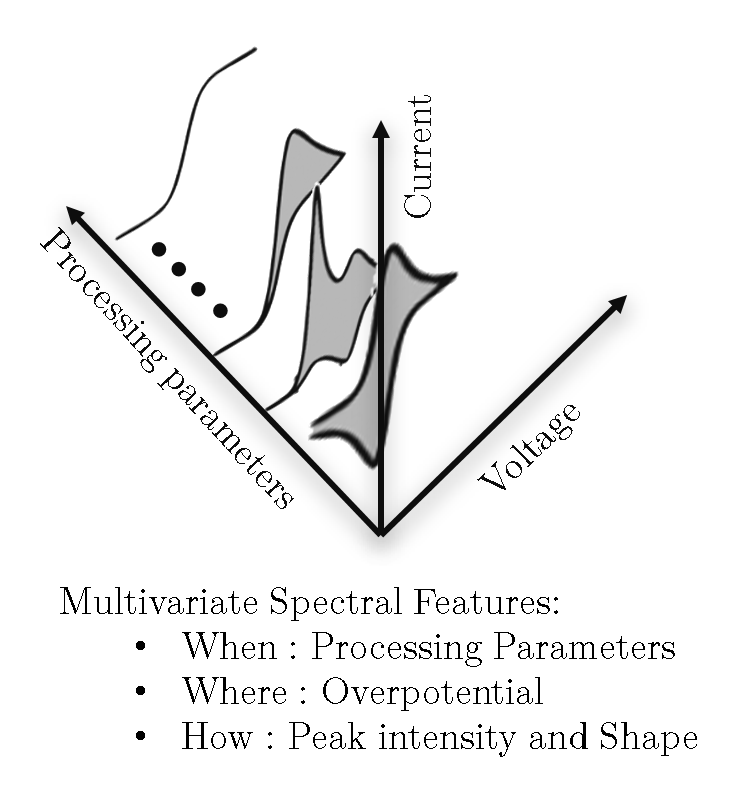
\includegraphics[width=0.45\columnwidth]{figures/spectral_hypercube.png}
    \caption{Hypercube of data from a typical cyclic voltammetry characterization of a catalyst material. Adapted from~\cite{rajan2013informatics}}
    \label{fig:spectrahypercube}
\end{figure}


Data based models emerged as an ubiquitous tool for analyzing high-dimensional signals, including in material science. In the data-driven science paradigm, data is used as a resource to extract knowledge from a highly complex systems often with a goal of identifying new phenomena that is not possible with manual human reasoning with in a reasonable time frame~\cite{brunton2019data}. We observe that data comes with two inherent properties: ~1) \textit{structure :} that assigns an arrangement~(often high dimensional) to each data point thereby capturing underlying governing characteristics of the sampled data that contribute to both local and global structure of dataset and ~2) \textit{stochasticity:} that assigns a probability to each data point that highlights relevance of a sampled data with in a context (for example an experiment). Encoding inherent properties of the data with a final goal of data analysis in mind is a key aspect often studied under the realm of \textit{representation}~\cite{bengio2013representation}. Structural representations are usually computed by assigning a metric space to the data, as it readily produces a notion of nearness and neighborhood that signifies an underlying local structure~\cite{mcinnes2018umap}. Other representations that encode a structure include graphs and simplicial sets for example. Representations that encode stochasticity of data points typically use a distribution of possibilities. Commonly used distributions include Gaussian~\cite{gardner2015bayesian,gavaghan2018use} and Poisson~\cite{flory1940molecular}.


We identify the following challenges from a  representation point of view:
\begin{itemize}
    \item {\textbf{Structure and Continuous data space: }Materials have an inherent connectivity about them as depicted in a periodic table for example, where each element is assigned an arrangement based on atomic number, electronic configuration and other recurring chemical properties~\cite{periodictable}. In general, this is true for data sampled from experiments or simulations over a property design space. Enforcing continuity constraints into data analysis of characteristic responses is a key challenge to understand the structure of the dataset~\cite{lebras2011constraint}}
    \item {\textbf{Stochasticity and Prior knowledge exploitation: } Responses from experiments involving synthesis and characterization can be assigned a probability of occurrence that is governed by underlying material characteristics such as a mechanism, crystal structure etc~\cite{hull2018stochasticity}. Encoding prior knowledge about stochasticity of a given characterization or synthesis of a material can greatly improve output of a data analysis and better guide data sampling.  For example, X-ray diffraction data analysis has greatly benefited from a representation that decodes each signal as a superposition of few basis patterns each representing a possible phase~\cite{Kusne2015HighthroughputDO,hattrick2016perspective}. For each signal with potential mixed phases, each pure phase is assigned a possibility of presence based on observed relative peak intensity giving rise to a stochastic representation used for deducing a phase mapping~\cite{gomes2019crystal,stanev2018unsupervised}}
\end{itemize}


 
\section{Research Objective}\label{sec1.2}
The research objective of this thesis is to identify and understand role of representation in the three tasks of accelerated material discovery; namely:~a) down selection;~b) autonomous experimental design;~c) property-response detection. 
Towards this the following research tasks are defined. The cyclic voltammetry responses is used as an example of complex, high-dimensional data with multiple representations possible for a task in hand. Phase diagrams of polymer blends are used as an example to determine design rules for solvent selection with applications in manufacturing of organic solar cells.
\begin{itemize}
    \item {\textbf{Research Task 1 }\textit{Down selection:} This task focuses on building a metric representation that encodes compositional connectivity into the structure of high-dimensional spectral data. We use a combinatorial CV dataset to understand the challenges in the context of obtaining a low-throughput of samples from an expert defined high-throughput search. With a goal to encoding compositional continuity to the high-dimensional structure of the data, we determine a mode diagram that is both useful for down selection and determination of property-response relations.}
    \item{\textbf{Research Task 2 }\textit{Autonomous knowledge extraction:} This task focuses on building stochastic or probabilistic representations of the data in the context of kinetic knowledge extraction from cyclic voltammetry. Extracting rate dependent performance measures of a catalyst is a bottleneck usually governed by unknown, complex underlying mechanisms. Extracting rate dependent performance measures of a (molecular)catalyst is typically a laborious process involving a grid search to identify "ideal" conditions to run an experiment that produces a catalyst response near its kinetic limits. We propose and show an empirical acceleration in data sampling by purely our selection strategy as a search of a particular probabilistic representation of CV curves.}
    \item{\textbf{Research Task 3 }\textit{Property-response map detection: } This task focuses on evaluating polymer mixtures based on their phase diagrams. We apply clustering method as an exploratory data analysis technique to the problem of solvent selection in organic solar cells. This task produces a data-driven alternative for experimental evaluation of compatibility of solvents for a given polymer-blend.}
\end{itemize}

The thesis is an accumulation of three papers~\cite{MLCD}, and it is structured as follows. 
Chapter 2 describes a metric learning approach for down selection of high-throughput spectral data with CV and XRD as examples. 
Chapter 3 describes a probabilistic representation of CV curves for actively searching for target CV shapes that are useful for extracting kinetic information. 
In Chapter 4 we use clustering of phase diagrams as a data driven alternative for solvent based manufacturing of organic solar cells. 
We conclude the thesis in Chapter 5.


\chapter{Down selection of high-throughput data}\label{chapter2}
In this chapter, we discuss challenges related to designing a data analytics tool for clustering high-throughput measurements performed on the compositional library of materials. 
The critical aspects of the proposed methodology are (i) learning the similarity measures, as opposed to using fixed similarity measures (e.g., Euclidean distance, dynamic time warping), while (ii) imposing the similarity in the composition space. 
The methodology presented in this chapter is based on the multi-task learning approach that is formulated to account for the composition neighborhoods of the compositional libraries.

The advantages of our methodology are demonstrated for the library of cyclic voltammetry curves generated for model multi-metal catalysts, as well as X-ray diffraction patterns from experimental studies.
The proposed approach is compared with the current state-of-the-art methods used in similar problems. 
This work has important implications for designing high-throughput exploration including catalysts for electrochemical systems, such as fuel cells and metal-air batteries. 

\section{Introduction}
The Materials Genome Initiative (MGI)~\cite{white2012materials,green2017fulfilling} stimulated progress in material screening to discover new materials at a fraction of the cost.  
To fully unlock the power of high-throughput material screening, three areas must be capable of fast and automated processing: material fabrication, characterization, and data analytics.
Significant progress has been made in the fabrication and characterization stages of the discovery process. 
For example, high-throughput inkjet printing has been used to make a library of materials and characterizing them (e.g., XRD diffractograms to identify atomic structure) in a matter of hours~\cite{koinuma2004combinatorial,takeuchi2002combinatorial}.
However, these advances have not been paralleled by the data analytic tools allowing knowledge extraction, and more important, the guidance for the next round of experiments. 

The data analysis of high-throughput experiments is particularly challenging due to the high uncertainty of the underlying physical phenomena related to the material properties, characterization details and the fabrication process itself. 
This is not surprising if one considers that little if any information, is known about screened materials including their behavior during the fabrication and characterization. 
In addition, if the physical laws guiding the extraction of material properties are undetermined or uncertain, data-driven approaches emerge as an apparent choice. However, these approaches may face significant challenges; for example, if design space is inadequately sampled (unknown a priori).  

In this chapter, several challenges related to the high dimensionality of measurements, choosing similarity measures and discovering sub groups in the data sets from high-throughput experiments are discussed.
The multi-task metric learning (MTML) is used to automatically learn a similarity measure of the experimental response data while respecting the composition similarity -- an important aspect to learn composition-response relationships for material libraries.
The MTML is a generic method to handle composition-response maps, but in this chapter, its robustness is demonstrated for two data sets:
(i) X-ray diffraction patterns to determine the phase diagram using experimentally collected data~\cite{long2007rapid}, and
(ii) cyclic voltammetry curves to determine highly correlated composition-response regions using synthetic data generated to mimic catalytic processes. 

\section{Background}
High-throughput exploration (HTE) starts with fabrication of the library of materials where the design variable is gradually sampled with some increment. 
For example, in a multi-component system, the composition of individual elements is varied resulting in the library of hundreds of samples~\cite{haber2014high}.
In the next step, a systematic characterization of each sample from the library is carried out. 
For example, X-ray diffraction patterns are measured to identify the atomic structure of synthesized samples~\cite{long2007rapid}. 
Compositional libraries with the XRD measurements have gained significant attention and have been analyzed using various techniques~\cite{Kusne2015HighthroughputDO,xiong2017automated}. 
This is not surprising as determining the phase diagram is the first step to understanding the behavior of the materials.
Finally, given the systematic material preparation and data collection, the goal for data analytic tools is to group the measurements such that materials in individual groups share some features in the measurements that inform the materials discovery process.
For example, in the case of XRD, the underlying assumption of this characterization is that phases emit a unique diffraction pattern, for example, the set of peaks. Hence, by identifying the set of unique patterns, the set of phases in the libraries can be determined. 
Moreover, the set of phases can be mapped to the samples in the compositional library and collectively represented as a phase diagram. 
However, due to the complexity of the XRD measurement (e.g., the diffraction data is collected in angular space to infer information about the lattice structure), the signal may be sensitive to lattice expansion or contraction, sample surface texture, etc~\cite{iwasaki2017comparison}.
For example, two samples with the same phase but small lattice distortion may give different XRD signals.
This may lead to the ambiguity in the interpretation, but also poses a challenge for data analytics. 
Specifically, the data analytics should be able to differentiate signals originating from different phases and cluster signals originating from the same phase while taking into account the susceptibility inherent to given measurement techniques. 
In practice, the comparison between individual signals is performed using some form of distance measure. 
Once distances are measured, the grouping can be performed such that object/samples similar to each other are grouped/clustered. 
GRENDEL~\cite{Kusne2015HighthroughputDO}, Gphase~\cite{xiong2017automated} have been introduced to tackle the problem of finding phase diagram from high-dimensional XRD diffractograms.  
Other approaches that do not directly involve clustering have been also applied. 
These approaches include constrained matrix factorization~\cite{bras2010computational} and a semi-supervised classifier SS-AutoPhase~\cite{bunn2016semi}. 
The former approach decomposes the diffractograms into basis patterns corresponding to individual phases. 
The latter approach uses a clustering algorithm to down select the representative diffractograms to be labelled by human. Using these labels, a classifier is trained to label the remainder of the diffractograms.
A comprehensive review of the existing methods to determine a phase diagram by clustering XRD data can be found in ~\cite{hattrick2016perspective}.

This discussion is not unique to phase diagram construction from XRD measurements. It is instead an example of a larger class of data analytics and unsupervised learning to discover composition-response maps.
The problem of grouping signals from high-throughput exploration to learn the properties of materials is generic to the materials screening and transpires into a myriad of characterization techniques. 
This work has been inspired by the cyclic voltammetry (CV) characterization to unravel electrochemical regimes in electrochemical systems, such as catalysts used in fuel cells and metal-air batteries.
In contrast to XRD data, a typical workflow for analyzing the libraries of CV curves involves extracting figure of merit (FOM) and seeking the trends across the compositional space to down select samples (i.e., make the transition from high-throughput to low-throughput)~\cite{haber2014high,haber2014discovering}. 
The goal of data analytics in such cases would be to find regions where a systematic variation in design space gives rise to systematic variation in response (e.g., composition regions with strong composition-response correlations). 
In \cite{suram2015generating} a genetic programming-based algorithm is introduced to find highly correlated composition-response regions in high-throughput CV data using an expert-defined FOM. 
However, this method has not been extended for high-dimensional responses. 

\subsection{Importance of distance measure}
Learning a relationship between a design variable (e.g., a composition of multi-metal oxide catalyst) and the response from HTE through data analytics faces several challenges. 
First, the measured responses from individual samples are typically represented as high-dimensional vectors (hundreds of measurements for each sample). A similarity measure between any two high-dimensional vector responses is defined using a distance metric to capture the statistical relation to its neighbors in the high-dimensional space that forms clusters.
This leads to the curse of dimensionality.
One of the consequences of this curse is that for the increasing number of dimensions, the distance from the query to its nearest and farthest may be similar~\cite{bellman1961curse}. 
In such cases, many distance functions are less effective. 
In particular, some distance functions produce uniform distances for data points similarly spaced apart in different dimensions.
Such ineffectiveness in identifying (dis)similar data points affects the clustering method. 
For example, it has been shown that the most popular Euclidean distance exhibits poor performance and is counter-intuitive for higher dimensions~\cite{aggarwal2001surprising}.
Selecting a proper similarity measure is more important in obtaining success with clustering than the clustering algorithm itself~\cite{friedman2001elements}. 
In an ideal case scenario, a good distance measure captures relationships between data points and produces well-separated clusters in some projected space, making clustering a fairly straightforward problem. 

The distance measure can be chosen from a large pool of canonical distance functions (e.g., Euclidean, Manhattan, Mahalanobis,  Minkowski, cosine), a distance between distributions (e.g., earth mover distance, Kullback-Leibler divergence) or hand designed distance functions (e.g., shape context matching). 
The above mentioned distance functions have been used for HTE studies as well~\cite{iwasaki2017comparison,hattrick2016perspective,hernandez2016using}.
A distance measure can also be learned from training data that are labeled. 
In such a case, the labeled data are used to narrow down features (e.g., dimensions) that are discriminant for the classes in the analyzed data set. 
For example, linear discriminant analysis (LDA) projects a data set onto a lower-dimensional space with good class-separability. 
Such a projection can be seen as finding a better representation of data (a pre-processing transformation) or considered as equivalent to the feature selection problem.

In real-life applications, including HTE, the labels are not easily available. 
This excludes many distance learning approaches and supervised techniques. 
However, a distance measure can still be learned if some form of domain-information exists to augment the data set. The domain information can be provided in terms of explicit labels or equivalence constraints~\cite{bar2005learning}.
For example, in the high-throughput exploration of composition libraries that are considered in this work, it is expected that samples that give similar responses should also be close in the composition space. 
In this sense, the composition of samples can be considered as a domain-information for the distance measure learning problem.

Once an appropriate similarity measure is computed, one can use off-the-shelf clustering methods such as agglomerative hierarchical clustering or, weighted graph partition, both of which rely on the similarity measure. A comprehensive discussion of clustering methods can be found elsewhere \cite{friedman2001elements}.

\par In this work, we adopt the state-of-the-art metric learning algorithm from machine learning to compute a physics-informed similarity measure. To our knowledge, this is the first attempt to learn a similarity measure for data analytics of material libraries. In particular, we demonstrate how learning a similarity measure can be posed as a multi-task metric learning (MTML) problem in machine learning.
We demonstrate the robustness of MTML for two types of measurements:
(i) the CV curves, as it directly motivated this work, and 
(ii) the Fe-Pd-Ga XRD data set~\cite{long2007rapid}, as it is a well-studied problem with several publicly available, expert-labeled data sets. 

\section{Method}
In this section, the workflow is described by first introducing metric as a distance function. 
The large margin nearest neighbor algorithm and its extension to the multi-task scenario is used to learn a metric. 
Next, the two concepts are coupled to learn the distance measure from HTE of compositional libraries.


\subsection{ Distance Metric Learning}
A metric is a mapping $D:V \times V \rightarrow R^+$. The map is a metric over a vector space $V$ only if it satisfies the following properties $\forall v_i,v_j,v_k \in V$:
\begin{enumerate}
    \item Triangular inequality:  $D(v_i,v_j)+D(v_j,v_k) \geq D(v_i,v_k)$
    \item Non-negativity: $D(v_i,v_j) \geq 0 $ 
    \item Symmetry: $D(v_i,v_j)=D(v_j,v_i)$
    \item Distinguishable: $D(v_i,v_j)=0 \iff v_i=v_j$
\end{enumerate}
Euclidean distance is a widely used example of a metric.
It is typically the first choice for supervised or unsupervised learning~\cite{dhanabal2011review,cover1967nearest}. 
A mapping $D$ can also be learned from the data to satisfy the properties mentioned above. 
A generalized Mahalanobis distance metric is one example of such a learned distance. Formally, the generalized Mahalanobis distance $D_M$ is defined as: 
\begin{equation}
    D_M (x_i,x_j) = \sqrt{(x_i-x_j)\mathbf{M}(x_i-x_j)^\top} 
                  = \sqrt{(\mathbf{L} x_i- \mathbf{L} x_j)(\mathbf{L} x_i- \mathbf{L} x_j)^\top}
    \label{eq1}
\end{equation}
where the matrix \(\mathbf{M}\) is a symmetric positive semi-definite matrix. Matrix \(\mathbf{M}\) is learned from data such that some constraints on the data are satisfied in addition to preserving properties required by the definition of the metrics. 
When \(\mathbf{M}\) is a positive semi-definite matrix, it can be decomposed as \(\mathbf{M=L^\top L}\).
In this sense, the generalized Mahalanobis distance measure ($D_M$) is equivalent to the Euclidean distance of the transformed data, where transformation $x\rightarrow \mathbf{L}x$ is learned from the data. 

Many works have reported ways to estimate \(\mathbf{M}\) for the problem at hand ~\cite{xiang2008learning,roth2014mahalanobis} with various linear and non-linear methods proposed to find metrics~\cite{kedem2012non}. Metric learning has been posed as a supervised or unsupervised problem demonstrating its versatility~\cite{wang2015survey}.  
In this work, we learn the distance metric using a large margin nearest neighbor (LMNN) algorithm~\cite{weinberger2006distance} that we detail in the next subsection. 

\subsection{Distance Metric Learning via LMNN}
LMNN learns a generalized Mahalanobis distance metric (\(\mathbf{M}\)) to improve \textit{k}-nearest neighbor classification of a single task over labeled high-dimensional data. 
Consider a data-label pair $(x_i,y_i)$, where $x_i \in R^d$ for $i=1,2,3,...,n$, and $y_i \in (1,2,3...,c)$. 
The data set consists of $n$ d-dimensional data points divided into $c$ classes. 
Learning a metric using LMNN is posed as a semi-definite problem of minimizing $D_M^2(x_i,x_j)$ where $x_i,x_j$ have the same label $y_i=y_j$ and penalizing $D_M^2(x_i,x_k)$ for $y_i \ne y_k$. This is achieved by solving the optimization problem stated as: 
\begin{equation}
\begin{aligned}
& \underset{\mathbf{M}}{\text{minimize}} &\sum\limits_{i,j\inS}{D_M^2(x_i,x_j)} +\mu \sum\limits_{S}{ \xi_{ijk} }\\
& \text{subject to}& \text{$i,j,k \in S=\{(i,j,k),y_i=y_j\ne y_k\}$ }\\
&                  & D_M^2(x_i,x_j)-D_M^2(x_i,x_k)\geq 1-\xi_{ijk}.\\
&                  & \xi_{ijk}\geq 0\\
&                   &\mathbf{M}\succeq 0\\
\end{aligned}
\label{eq2}
\end{equation}
LMNN finds a matrix \(\mathbf{M}\) such that for a given data point $x_i$, points in the local neighborhood of $x_i$ are separated between classes and brought close for within classes. 
LMNN assumes that the set of $k$ nearest neighbors for a given query data point come from the same class as the query. These neighbors are called target neighbors. The LMNN algorithm uses the knowledge about the target neighbors to learn distance \(\mathbf{M}\) such that target neighbors are closer to each other than to the data points from another class (also called impostors) -- by a large margin.
The choice of the nearest neighbors is typically made using some side-information, or in the absence thereof, the Euclidean distance between data points is used to identify $k$ nearest neighbors from within a given class~\cite{weinberger2006distance}. One of the advantages of LMNN is that it considers the local information by imposing constraints in a local manner.

\subsection{Distance Metric Learning via MT-LMNN}
Multi-task learning (MTL) is a sub-field of machine learning. It is based on the assumption that if several tasks are related, then co-learning these tasks improves learning performance. 
MTL can be seen as \textit{inductive transfer learning} where discovering the relationships among different but related tasks serves as inductive bias to improve the learning~\cite{caruana1997multitask}. 
The MTL paradigm is generic and can be used for various problems such as supervised learning (e.g., classification or regression problems), unsupervised learning (e.g., clustering), graphical models, etc.
In this work, we use the multi-task LMNN algorithm to learn a metric in MTL framework ~\cite{parameswaran2010large}. 

MT-LMNN learns a shared metric (defined by \(\mathbf{M_0}\)) and a task-specific metric (defined by \(\mathbf{M_t}\)) such that \textit{k}-nearest neighbor classification is improved for each task while capturing general trends in \(\mathbf{M_0}\). A single metric that improves the classification for a given task $t$ is defined as \(\mathbf{M_{0} + M_{t}}\).
The regularized loss minimization principle is used to learn  \(\mathbf{M_0}, \mathbf{M_t}\) according to the following:
\begin{equation}
\begin{aligned}
& \underset{\mathbf{M_0,M_1,...,M_T}}{\text{minimize}} &\gamma_0\lVert \mathbf{{M_0-I}} \rVert ^2_F+ \sum_{t=1}^{t=T} \gamma_t \lVert \mathbf{{M_t-I}} \rVert ^2_F\\
\end{aligned}  
\label{regM}
\end{equation}
where $t=1,2...,T$ represent different tasks being defined on the data, and $\gamma_i (i=0,1,2...,T)$ are regularization coefficients. 

In this work, we build on the assumption that in composition libraries the material properties along and across compositional dimensions are related within some local neighborhood. 
Specifically, if one considers the phase diagram for a ternary system, there will be some commonalities between material properties (or associated measurements such as XRD) when screened along three compositional dimensions.
If these commonalities are captured in the multi-task setting, the distance measure can be learned more efficiently (defined by \(\mathbf{M_0}\), and \(\mathbf{M_t}\)) and subsequently can inform the clustering algorithm.

In the original paper~\cite{parameswaran2010large}, MT-LMNN was formulated as a classification problem and required classes to be defined. 
Two sets of problems were considered, label-compatible tasks (where the tasks share the same label set) and label-incompatible tasks (the tasks do not share a label set). 
In this work, we choose the definition of classes and tasks such that each task corresponds to one design variable (e.g., elemental composition) and each class corresponds to a category of the design variable (e.g., low, medium and high chemical content of the corresponding element). 
Such a problem definition applies to the HTE data of a multi-component composition library, where each sample is characterized by (a)~some measurement to generate a response curve and (b)~elemental compositions being the design variable. 
Consequently, the number of tasks is defined by the number of elements screened in HTE.
For the same data, each task has a set of incompatible labels.
Each label is defined as a category representing the relative content of the corresponding element within some interval.
For example, three categories can be chosen for a given elemental content: low, medium and high. 
In general, one can divide the data into a finite number of various classes ($c$) by sorting the data according to the design variable. In this work, the response is divided into three categories of low, medium and high elemental content. This results in three classes for each task. Without loss of generality, one can aim to find the optimal number of classes. 

MTL with tasks and classes defined as above is used to learn a metric using MT-LMNN to improve the classification in each task (corresponding to individual elements). 
MTL is formulated such that it improves the learning of distance on classes defined based on the element content. 
The relative value of regularized coefficients $ \gamma_{0t} = \lVert \gamma_0 -\gamma_t \rVert$ signifies the importance of each task specific metric \(\mathbf{M_t}\) over shared metric \(\mathbf{M_0}\) to improve \textit{k}-nearest neighbor classification for task $t$. 
A lower value of $\gamma_{0t}$ means that the shared metric \(\mathbf{M_0}\) is sufficient to classify data points for task $t$.  
One can select the regularization coefficients in~\Cref{regM} through hyperparameter selection using a constrained Bayesian optimization to minimize \textit{k}-NN classification error (see Supplementary Information for more information). 
Intuitively, if regularized coefficients are selected, metric learning results in a single shared metric \(\mathbf{M_0}\) that finds general trends in the data while accurately classifying data points for all tasks. 
This is equivalent to learning a similarity measure for the high-dimensional responses, which respects the similarity in terms of the composition (i.e., since \(\mathbf{M_0}\) can classify data points based on relative chemical content for all the elements, it knows the relative location of a data point in composition space).   

Once a metric \(\mathbf{M_0}\) is learned via MT-LMNN, it is used in conjunction with the off-the-shelf clustering algorithms to find clusters in the design space. The generic workflow proposed in this paper consists of the following steps: 
\begin{enumerate}
\item Data obtained from HTE is stored in a matrix $X$ (each column is a response for each sample).
\item A generalized Mahalanobis metric \(\mathbf{M_0}\) is learned on $X$ such that it emphasizes similarity in terms of response as well as a design variable (composition).
\item Clustering method is used to group the samples into clusters using the similarity measure computed earlier. We use a (i) hierarchical clustering algorithm (HCA) and (ii) weighted graph partition algorithms for demonstration purposes. 
\end{enumerate}
\section{Results and discussion}
%%%%%%%%%%%%%%%%%%%%%%%%%%%%%%%%%%%%%%%%%%%%%%%%%%%%%%%%%%%%
In this chapter, the robustness of the MTML is demonstrated for compositional libraries using two types of measurements. 
First the analysis of synthetic cyclic voltammetry curves is reported.
Synthetic data is generated with characteristic features explicitly dependent on the material composition. 
In the second case, the experimental data set from the XRD experiment that has been labeled by the human expert~\cite{long2007rapid} is used. 
Two two data sets are diverse and serve as a good test for MTML.

%%%%%%%%%%%%%%%%%%%%%%%%%%%%%%%%%%%%%%%%%%%%%%%%%%%%%%%%%%%%
\subsection{Composition-response maps from cyclic voltammetry}

\subsubsection{Data generation}
The synthetic data is generated such that it mimics electrochemical data from a cyclic voltammetry test. 
Inspired by the works in~\cite{saveant1980catalysis,costentin2017catalysis}, where the solutions of electrochemical reaction system models are predominantly exponential functions, we choose to generate response $X_i$ using an affine combination of Gaussian functions as follows:

%\begin{equation}
%    X_i = \frac{D2}{7.98}\cdot\frac{1}{{\sigma _1 \sqrt {2\pi } }}e^{{{ - \left( {x - D1 } \right)^2 } \mathord{\left/ {\vphantom {{ - \left( {x - D1} \right)^2 } {2\sigma _1 ^2 }}} \right. \kern-\nulldelimiterspace} {2\sigma _1 ^2 }}}+\frac{D3}{0.54}\cdot\frac{1}{{\sigma _2 \sqrt {2\pi } }}e^{{{ - \left( {x - 1.2 } \right)^2 } \mathord{\left/ {\vphantom {{ - \left( {x - 1.2 } \right)^2 } {2\sigma _2 ^2 }}} \right. \kern-\nulldelimiterspace} {2\sigma _2 ^2 }}}
%    \label{eqGauss}
%\end{equation}

\begin{equation}
\begin{split}
X_i(x)=\frac{D2}{g(D1,D1,\sigma_1)} g(x,D1,\sigma_1) + \frac{D3}{g(1,D2,\sigma_2)} g(x,1.2,\sigma_2) \\
g(x,\mu,\sigma)= \frac{1}{{\sigma \sqrt {2\pi } }}e^{{{ - \left( {x - \mu } \right)^2 } \mathord{\left/ {\vphantom {{ - \left( {x - \mu } \right)^2 } {2\sigma^2 }}} \right. \kern-\nulldelimiterspace} {2\sigma ^2 }}}
\end{split}
    \label{eqGauss}
\end{equation}
The model is built as the sum of two Gaussian functions ($g(x,\mu,\sigma)$) over the normalized domain $x\in(0,1)$ with mean ($\mu$) and standard deviation ($\sigma$) chosen according to the material composition in the HTE library. 
For each sample of a given composition, a signal is generated using an explicit function (see ~\Cref{DOFsVar}). 
The union of all the responses gives rise to a data matrix $X_{m\times n}$ where $m$ is the dimensionality of the response and $n$ is the total number of samples (we use $m=350$,$n=435$). 

The signal consists of a single peak followed by the exponential increase to the cut-off value. 
The shape of the signal is controlled by three degrees of freedom (DOF): $D1$, $D2$ and $D3$. 
Three degrees of freedom are equivalent to the features of the signal: the position of the peak, the peak intensity, and the cut-off value.
Specifically, the position of the first peak is controlled by $D1$, its intensity by $D2$, and the cut-off value by $D3$, respectively.
The remaining DOFs are kept fixed: $\sigma_1=0.05$, $\sigma_2=0.1$ and the mean value of the second Gaussian function in~\Cref{eqGauss} is set as $1.2$ to be outside of the normalized time frame. 
The right panel of~\Cref{datsExpl} depicts the example signal with a degree of freedom marked and added noise. 

Parameterizing the signal with the finite number of DOFs allows us to connect them with three compositions in ternary libraries directly. 
Assuming that each sample in a ternary system consists of three elements with composition $C = (C1,C2,C3)$ (see \Cref{DOFsVar}), the mapping between design variables ($C$) and the shape of the signal can be explicitly defined. 
Moreover, multiple mappings can be defined for a given multi-component system. 
Each mapping is defined over a subset of design space, which we call phase. 
This subset may have a physical meaning. 
For example, in the case of the library with XRD measurements, the subset is equivalent to samples of the same phase (in terms of the same lattice structure). 
In a more general case, an individual subset is a group of samples from the continuous neighborhood in the design space.
Above definition of a subset mimics the down selection map of a HTE CV data by Suram et al~\cite{suram2015generating}. 
However, here we parameterize the signal with three DOFs and work with resulting high-dimensional responses, while in~\cite{suram2015generating}, one figure of merit -- overpotential -- was selected as a feature of the CV signal. 
%which have a unique trend for the three DOFs combined. A typical response curve generated using these parameters is shown in~\Cref{sampData}. 

 \begin{figure}[h]
    \centering
    \begin{subfigure}[b]{0.475\textwidth}
        \centering
        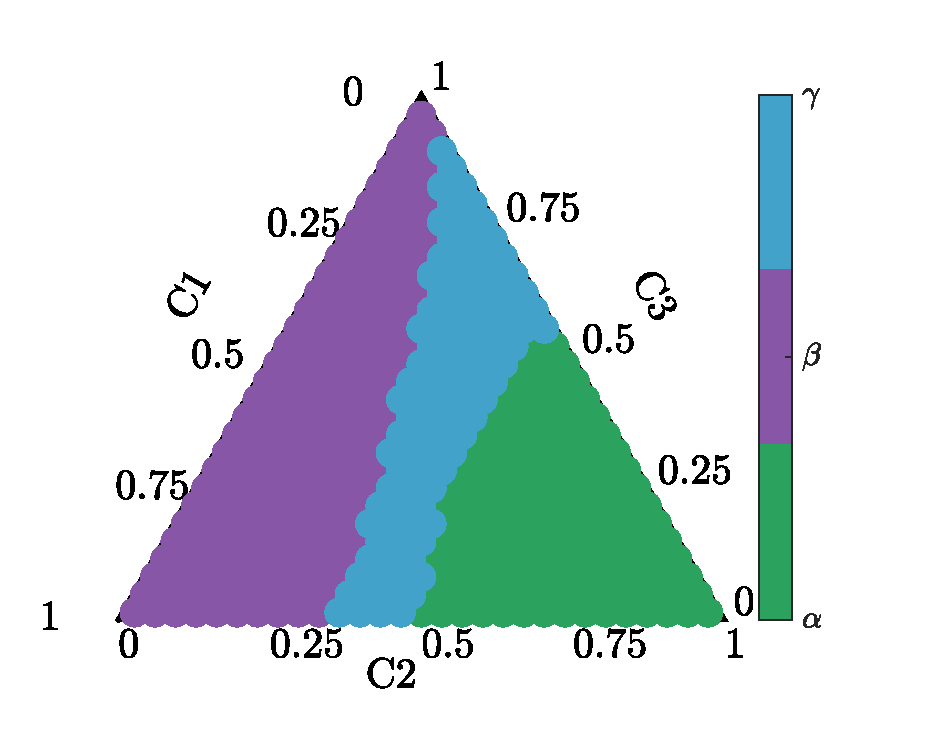
\includegraphics[width=\textwidth]{Chapter-2/figs/Figure1a.eps}
        \caption{}
        \label{origPhase}
    \end{subfigure}
    \quad
    \begin{subfigure}[b]{0.475\textwidth} 
        \centering 
        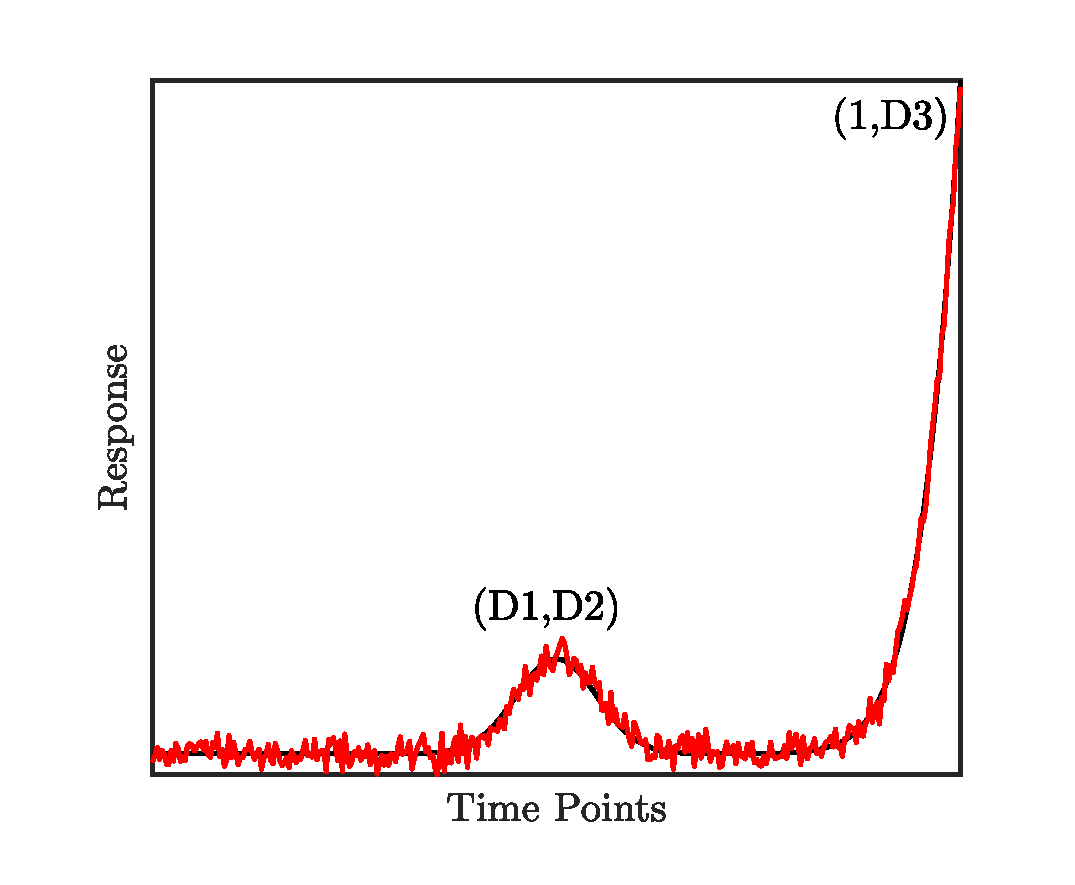
\includegraphics[width=\textwidth]{Chapter-2/figs/Figure1b.eps}
        \caption{}
        \label{sampData} 
    \end{subfigure}
    \vskip\baselineskip
    \caption{(a) Ternary sample with elemental compositions given as C1, C2, C3; partitioned into three known phases. Each color corresponds to one phase. (b) A typical high-dimensional sample response in the synthetic data (red--with Gaussian noise). The degrees of freedom are denoted as D1 (peak position), D2 (peak intensity), D3 (cut-off current)}
    \label{datsExpl}
\end{figure}

\begin{table}[h]
     \centering
\begin{tabular}{|l|l|l|l|l|l|l|}
\hline
& \multicolumn{3}{ |c| }{\textbf{Non-Separable DOFs}} &\multicolumn{3}{ |c| }{\textbf{Separable DOFs}}\\ \hline
Phase in \Cref{origPhase} & D1 & D2 & D3 & D1 & D2 & D3 \\  \hline
\textbf{$\alpha$} & C2+C3 & C3 & 2+C2 & C2+C3 & C3 & 2+C2 \\ 
\textbf{$\beta$} & C2 & C1+C2 & 2+C1 & C2 & C1+C2 & 4+C1 \\ 
\textbf{$\gamma$} & C3 & C1 & 5.0 & C3 & C1 & C1+C3 \\ 
\hline
\end{tabular}
     \caption{DOF variations across each phase for two cases considered in the data sets.}
     \label{DOFsVar}
 \end{table}


\begin{figure}[h]
    \centering
    \begin{subfigure}[b]{0.475\textwidth}
        \centering
        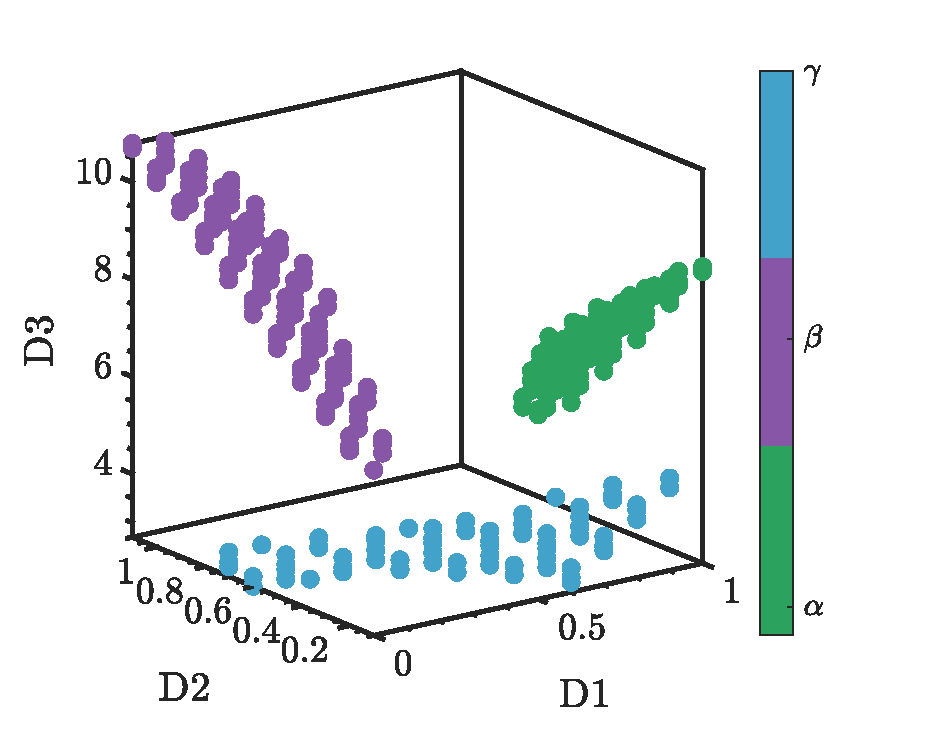
\includegraphics[width=\textwidth]{Chapter-2/figs/figure2a.eps}
        \caption{}
        \label{sepDOFscate}
    \end{subfigure}
    \quad
    \begin{subfigure}[b]{0.475\textwidth} 
        \centering 
        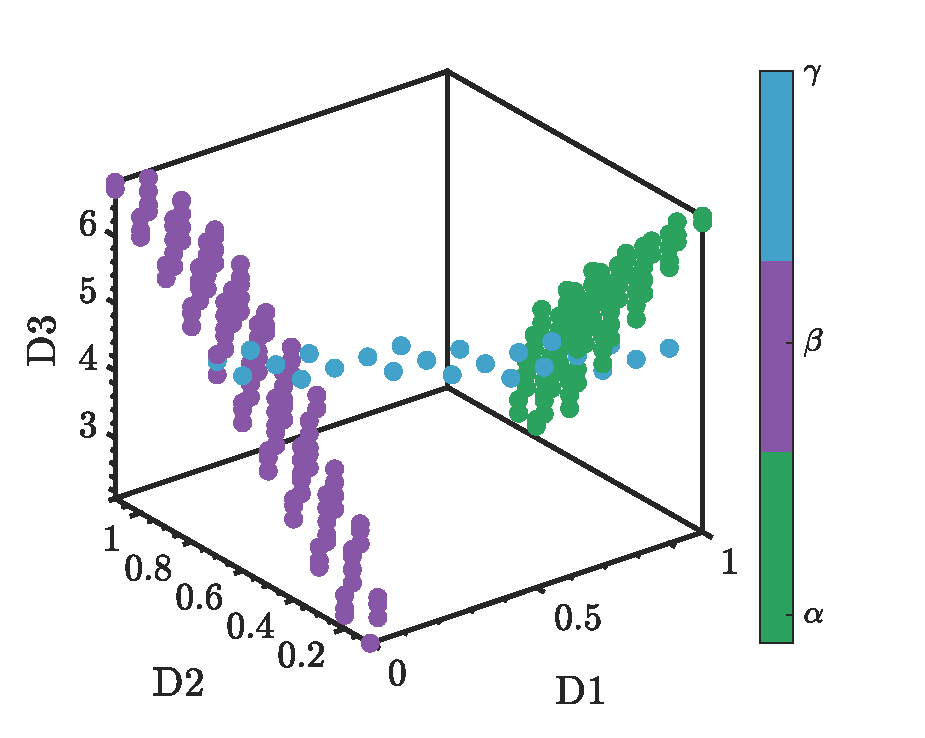
\includegraphics[width=\textwidth]{Chapter-2/figs/figure2b.eps}
        \caption{}
        \label{nonsepDOFscate} 
    \end{subfigure}
    \vskip\baselineskip
    \caption{(a) Phases can be clearly separated in the three dimensional known DOF space (Test cases SET A1,B1) (b) phases can not be separated clearly in three dimensional space (Test cases SET A2,B2)}
    \label{scates}
\end{figure}

% In general, for any given $m$--dimensional HTE data response matrix $X_{m \times n}$ and its corresponding composition matrix $C_{3 \times n}$, its governing $l$--dimensional degrees of freedom matrix $D_{l \times n}$ can be defined using a map $M_{DX}: D_{l\times n} \rightarrow X_{m\times n}$. 
% Learning a compositional phase diagram would require one to partition the map $M_{DX}$ into a set of surjective maps $P_k$ on the data set $\mathcal{D} = (X_{m \times n},C_{3 \times n})$ such that $P_k: \mathcal{C}_{k} \rightarrow \mathcal{X}_{k}$ is continuous in $\mathcal{C}_k \subset C$ for the corresponding $\mathcal{X}_k \subset X$.
% Maps $P_k$, defined above, may result in an irreducible representation (typically a lower dimensional manifold) such that: (1)~the responses form distinct clusters in the lower dimensional embedding ; that is, $P_k$ are distinct  $\forall k $ and $M_{DX}$ is continuous in $C$, or (2)~the responses are overlapping; that is, $P_k$ are distinct $ \forall k $ but $ M_{DX} $ is discontinuous in $C$.
% \begin{figure}[H]
%     \centering
%     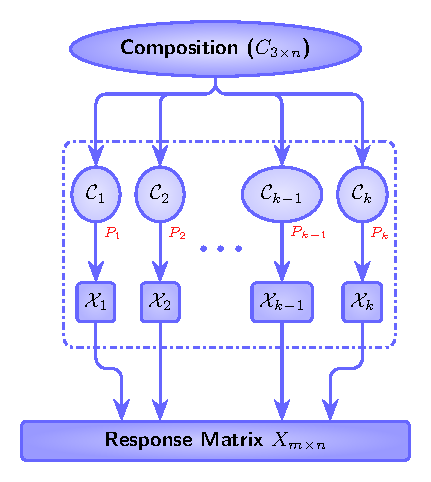
\includegraphics[width=0.5\textwidth, angle=0]{Chapter-2/figs/CompPhaseMap.pdf}
%     \caption{A composition-response map can be seen as a partitioning of the map $M_{DX}$ into various maps $P_k$}
%     \label{compPhaseMap}
% \end{figure}

% Distinct, continuous maps physically signify the dependency of responses entirely on composition (e.g., XRD structural data~\cite{long2007rapid,iwasaki2017comparison}). Presence of a discontinuous map $M_{DX}$ means that at least some responses are not completely governed by composition. In other words, there are at least two samples with similar responses  that are widely separated compositions in the composition space (e.g, cyclic voltammetry data where the overpotential, one of the degrees of freedom of the response, is surjectively mapped to composition with several samples having similar values of overpotential but are very widely separated in composition space~\cite{suram2015generating}). 
%However, we would like to note here that, since composition is not the only variable that governs the response, it is reasonable to assume that for a given phase map $P_k$, some of the governing DOFs of subset of responses $ \mathcal{X}_k$ may not depend on the corresponding composition subset $ \mathcal{C}_k$. Non-existence of map $P_k$ results in an irreducible representation of data (typically a lower dimensional manifold) that does not clearly separate the inherent clusters or phases exist in the data as it has not captured the properties of exact phase map $P_{k}^{E}:D_{l \times n} \rightarrow X_{l \times n}$.%

In this chapter, a data set $\mathcal{D}$ is generated with $k$ phases. Two cases with varying degrees of difficulty are considered.
In each case, three maps for each $k \in \{ 1,2,3 \}$ (see ~\Cref{DOFsVar}) is defined such that the ternary composition space has three inherent non-hyperspherical subsets (e.g., parabolic cuts as shown in~\Cref{origPhase}). 
% Two cases are considered: (1)~the case of separable DOFs that mimics the existence of three distinct surjective phase maps $P_k$, $ \forall k = \{1,2,3\}$ such that $M_{DX}$ is continuous in $C$; and (2)~the case of non-separable DOFs that mimics the discontinuous nature of $M_{DX}$ in $C$ with a set of phase maps such that $P_k$ does not completely represent the respective subset of the $M_{DX}$ map for at least one $k \in \{ 1,2,3 \}$.

The first case, separable DOFs, consists of data points $\mathcal{X}_k$ forming distinct clusters, such as the one shown in~\Cref{sepDOFscate}. 
% This is equivalent to having three distinct maps partitioning the data (i.e., equivalently partitioning the high-dimensional manifold of $X_{m \times n}$) such that mapping is bijective and each composition has a unique response. 
% Formally, $\mathcal{X}_i \bigcap \mathcal{X}_j = \varnothing $, $\forall \mathcal{X}_i, \mathcal{X}_j, i \neq j$, where $\varnothing$ is an empty set. % (Note that since $\bigcap$ is taken for subsets with high dimensional responses as elements, it uses the similarity measure $S$ defined earlier to identify if two responses are same).
% As shown in~\Cref{DOFsVar}, each phase in the separable DOF case is assigned distinct, surjective maps $P_k$ that define DOFs and the corresponding responses $\mathcal{X}_k$.
~\Cref{sepDOFscate} depicts the relationships between DOFs for three maps we used in this work.
The DOFs of each map are marked with a different color. 
In this case, there is no overlap in DOF space between distinct phases.
This clear separation between DOFs makes this data set simpler to analyze with better performance -- as shown in the results section. 
%in the irreducible representation using standard distance metrics since the responses have highly correlated and distinct clusters governed by the corresponding maps $P_k , k = \{ 1,2,3 \}$.
The second case, non-separable DOFs, consists of maps resulting in data points that are not separable on the manifold with DOFs as basis vectors.
% This is equivalent to having three distinct maps $P_1,P_2,P_3$ that divide the data such that $\exists  i, j$ and $\mathcal{X}_i \bigcap \mathcal{X}_j$ is a non-empty set for $ i \neq j \in \{1,2,3\}$.
% ~\Cref{DOFsVar} lists three maps for the non-separable DOF case that we used in this work. 
% Individual phases are named $\alpha$, $\beta$ and $\gamma$. 
% Both phases $\alpha$ and $\beta$ have injective maps $P_{\alpha}$, $P_{\beta}$ that define DOFs where the values of the DOFs do not overlap. 
% This is depicted in~\Cref{nonsepDOFscate}. 
% However, maps $P_{\gamma}$ are defined such that their DOFs overlap with the DOFs defined by two other phases.
% This overlap in DOFs and corresponding data points for $P_{\gamma}$ leads to the case where the inherent phases exist in the data, but their DOFs are not separable, thus making the standard metrics ineffective. (See Supplementary Information for a pictorial representation of the DOFs variation for both types of synthetic data sets.)
With the direct problem stated as above, the goal is to identify the inherent clusters from the high-dimensional data $X$.
% In this work, we aim to learn a metric that closely represents the maps $M_{DX}$ and $P_k$ , where the map $M_{DX}$ represents the inherent clusters in the high-dimensional data $X$, and maps $P_k$ impose constraints relevant to the compositional continuity in $C$. 
% This continuity constraint motivates the similarity measure that combines similarity in response space as well as the nearest neighborhood in the corresponding composition space.
%We generate two sets of synthetic data with varying degree of complexity.
%In both cases, we generate response curves such that ternary composition diagram is divided into three subsets (phases) with three distinct maps: $P_k: C_{3\times n} \rightarrow D_{3 \times n}$ where $k=1,2,3 $ for each of the three phases shown in ~\Cref{origPhase}.

\begin{table}[h]
     \centering
\begin{tabular}{ |l|l| }
  \hline
  \multicolumn{2}{|c|}{Test data sets} \\
  \hline
  SET A1 & Separable DOFs \\
  SET A2 & Non-Separable DOFs \\
  SET B1 & Separable DOFs, Noisy data $\sim \mathcal{N}(0,0.1)$ \\
  SET B2 & Non-Separable DOFs, Noisy data $\sim \mathcal{N}(0,0.1)$ \\
  \hline
\end{tabular}
    \captionsetup{justification=centering}
     \caption{Description of data sets used for evaluation. Gaussian noise is added with variance approximately 10 \% of the peak intensity}
     \label{datasets}
 \end{table}
 
\subsection{Comparison between several distance measures}
To learn a metric for data matrix $X$ using the framework introduced earlier, each element in the ternary space is considered as a task. 
For a ternary system, three tasks are considered. 
In each task, we define a class by sorting the data points based on corresponding element content and sequentially categorizing the data point.
The generated data set consists of 435 data points, giving four classes for a given task (each class consists of 100 points, with the remaining 35 points in the last class added to the penultimate class).
The procedure is repeated for the remaining tasks, giving three sets of incompatible labels.

We will now compare distance metric learned in the MT-LMNN framework (with tasks and classes defined as above) with other commonly used distance measures such as Euclidean, cosine metrics, correlation, dynamic time warping (DTW), etc. 
% \begin{itemize}
%     \item Hierarchical clustering algorithm (HCA) with three different linkage options (average, complete, single) with varying number of clusters
%     \item  Spectral clustering method\cite{ng2002spectral,zelnik2005self} to partition the graph generated on the composition data with weights defined by a similarity measure. The graph is generated using either the 10-nearest neighbor algorithm or Delaunay tessellation. Local scaling of similarity measure mentioned in~\cite{zelnik2005self} is varied from two to six along with a varying number of clusters.
% \end{itemize}
For each metric, we use two sets of clustering algorithms (detailed below), with various settings possible:
\begin{itemize}
    \item Hierarchical clustering algorithm (HCA) with three different linkage options (average, complete, single) with varying numbers of clusters(for example,~\(\{k_0-1,k_0,k_0+1\}\) where $k_0$ is actual number of clusters).
    \item  Spectral clustering method\cite{ng2002spectral,zelnik2005self} to partition the graph generated on the composition data with weights defined by a similarity measure. The graph is generated using either the 10-nearest neighbor algorithm or Delaunay tessellation. Local scaling of similarity measure mentioned in~\cite{zelnik2005self} is varied from two to six along with a varying number of clusters (for example,~\(\{k_0-1,k_0,k_0+1\}\) where $k_0$ is actual number of clusters).
\end{itemize}

Clustering is selected as a indirect way of evaluating the performance (and importance) of a distance measure. In general, clustering aims to find homogeneous subgroups such that data points in each cluster are similar according to the similarity measure.
If the distance measure can capture the key features defining the similarity (in the context of the output quantity), the subgroups can be separated, and clustering will provide insight into data.
If informative features are selected, clustering is an appropriate technique to find subgroups in the input data.

The accuracy of clustering is evaluated based on the F-measure calculated using~\Cref{eq41}:
\begin{equation}\label{eq41}
    \begin{aligned}
    & F = \sum_{i=1}^{k} \frac{\abs{A_i}}{N} \underset{j}{\text{max}}  \frac{2R_{ij}P_{ij}}{R_{ij}+P_{ij}}\\
    & P_{ij}=\frac{\abs{A_i\cap B_j}}{\abs{B_j}}\\
    & R_{ij}=\frac{\abs{A_i\cap B_j}}{\abs{A_j}}
    \end{aligned}
\end{equation}
where $\abs{\mathcal{A}}$ returns the number of elements in the vector $\mathcal{A}$; $N$ is the total number of samples; $P$ is the precision and $R$ is the recall.
To calculate the F-measure, pre-defined labels ($A_i$) for phase $i$ are used to compare with labels from the graph partitioning $B_j$.  
Intuitively, the F-measure evaluates if a group of samples are clustered the same as the known clusters (or phases). 
If all samples were classified correctly, the F-measure equals one. 
The lower the value of this measure, the poorer the classification performance. We report the mean value and standard deviation of the F-measure from various clustering settings mentioned above as the stochastic performance measure of the metric on any given data set. This is performed to alleviate any inconsistencies in the F-measure that may arise from various clustering settings. The standard deviation in stochastic F-measures quantifies the consistency (or stability) of clustering for a given distance measure.  This way of looking at the data helps to quantify the effect of the metric on learning a response map.

%{\color{red}In general, the clustering performance is difficult to evaluate~\cite{caruana2006meta}. Several approaches (including F-measure) are being used with their strengths and weaknesses.We list alternative clustering performance evaluation in the Supplementary Information. However, F-measure is the most widely used and accepted by the community~\cite{manning2010introduction}. }

\begin{figure}[h]
    \centering
    \begin{subfigure}[b]{0.475\textwidth}
        \centering
        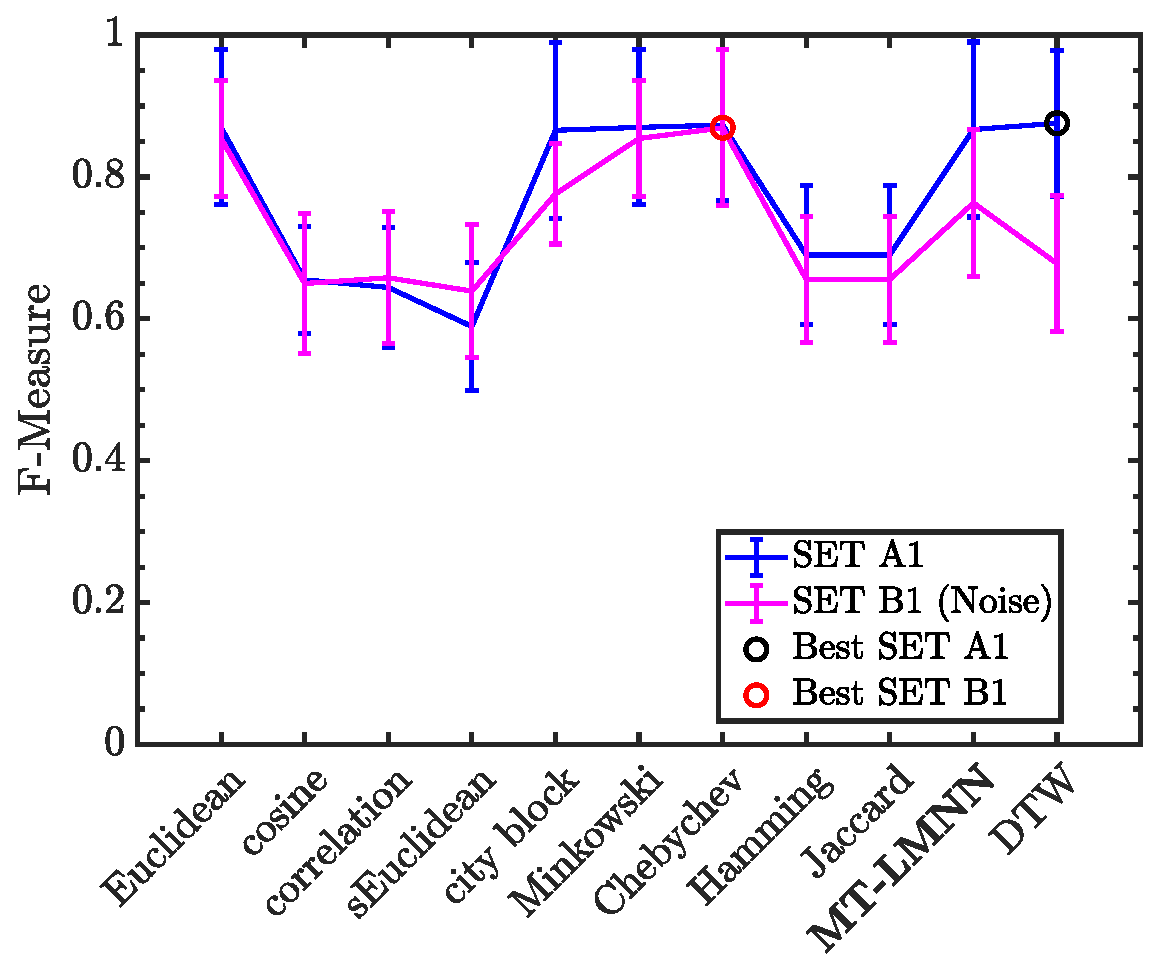
\includegraphics[width=\textwidth]{Chapter-2/figs/SD.eps}
        \caption{Separable DOFs}
        \label{errSD}
    \end{subfigure}
    \quad
    \begin{subfigure}[b]{0.475\textwidth} 
        \centering 
        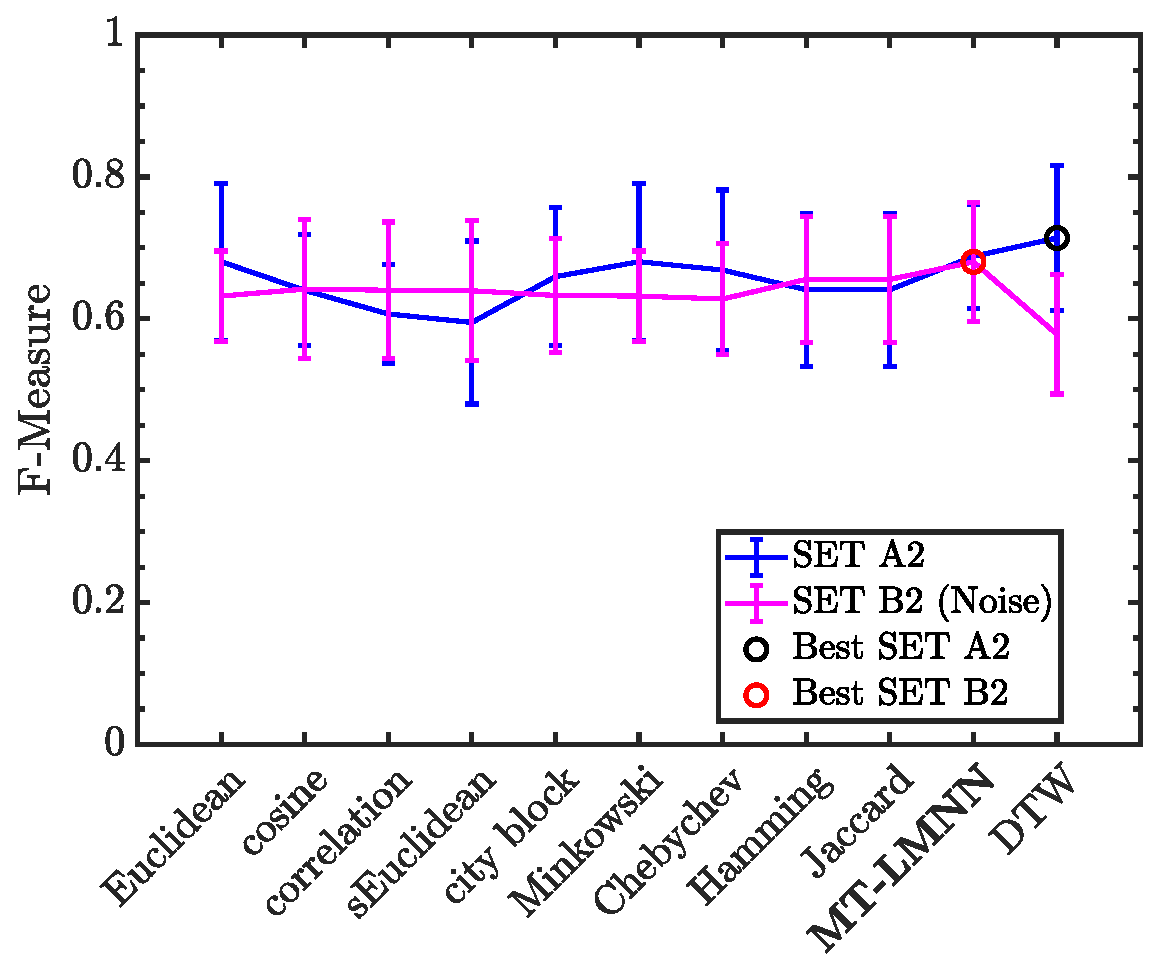
\includegraphics[width=\textwidth]{Chapter-2/figs/NSD.eps}
        \caption{Non-Separable DOFs}
        \label{errNSD} 
    \end{subfigure}
    \vskip\baselineskip
    \caption{F-measure statistics suggest that the similarity measure learned using MT-LMNN is at least as good as the best similarity measure obtained from exhaustive search over several metrics in all cases. We used Euclidean, cosine, correlation, standardized Euclidean (sEuclidean), city block, Minkowski, Chebychev, Hamming, Jaccard and dynamic time warping (DTW)  for an exhaustive similarity measure search.~\Cref{errSD} corresponds to separable DOFs case,~\Cref{errNSD} corresponds to non-separable DOFs case as described in the text.}
    \label{errorsDataNoise}
\end{figure}

\Cref{errorsDataNoise} contains the comparison between the performance of several distances and the approach taken in this work, MT-LMNN. 
The comparison is performed for two data sets with separable (A1) and non-separable DOFs (A2). 
Two additional data sets are analyzed with the noise added (data sets annotated with B - see Table~\ref{datasets}). To calculate F-measure statistics, we vary the number of clusters from two to three for all the cluster settings mentioned above.  

Our analysis shows that the similarity measure learned using MT-LMNN augments the ability to find regions with high composition-response correlation.
MT-LMNN is at least as good as the best distance measure obtained from an exhaustive search sometimes outperforming the complex, more sophisticated dynamic time warping (DTW). % Unlike DTW (which has the best stochastic F-measure in SET A1, A2 ), MT-LMNN is insensitive to the effect of noise (SET B2). %
We also note that analysis of each of the four data sets considered in~\Cref{datasets} resulted in four different measures as the best. However, MT-LMNN's performance was comparable to the best distance measure for SET A1, A2 (i.e., DTW) while producing the best accuracy in SET B2 (complex data set of the four). This also highlights the ability of MT-LMNN to quantify similarity automatically without any expert knowledge about the data that is required to select DTW or Chebychev.

We attribute the excellent performance of MT-LMNN to the local learning characteristics. 
The metric is learned in a small local neighborhood of each data point (determined by its classes). Learning a metric locally in a small neighborhood defined by the design space variable helps the clustering method to identify phases where the data responses are highly correlated but undergo systematic variation with the design space.
Results presented in this work demonstrate that this approach is robust even for the variation in degrees of freedom over a large range of composition. 

We would like to note that although the F-measure is widely used and accepted by the community~\cite{manning2010introduction}, it may not represent a pure performance of clustering~\cite{powers2015f}. However, there is no other good alternative to address the performance of clustering. 
To check if different conclusion is reached for other clustering performance measures, we performed the analogous analysis for other measures. 
We performed the analysis for four other performance measures: the adjusted rand index, the adjusted mutual information, the normalized mutual  information and Fowlkes-Mallows scores. 
Interestingly, regardless of selected performance evaluation measure, we reached the same observation. 
We additionally performed the one-sided paired t-test between MT-LMNN and the best metric.
We designed the hypothesis test to classify how similar (or dissimilar) are two metrics in terms of any given clustering performance measure distribution over clustering settings that are varied.  
Our additional analysis reiterates the main conclusion that MT-LMNN is at least as good as the best distance measure obtained from the exhaustive search.

\input{Chapter-2/sup_ttest}

%%%%%%%%%%%%%%%%%%%%%%%%%%%%%%%%%%%%%%%%%%%%%%%%%%%%%%%%%%%%%%%%%%%%%%%%%%%%%%%%%%%%%%%%%%%%%%%%%%%%%%%%%%
\subsection{Phase diagram construction from XRD measurements}

\subsubsection{Data description}
In this section, we use the labeled data sets by Long et al. \cite{long2007rapid}. 
This data set corresponds to the ternary library of Fe-Pd-Ga prepared by elemental sputtering. 
The data set contains 278 diffractograms (each of 1616 dimensions), and the corresponding composition map. 
The diffraction patterns are collected in 1D intensity versus 2$\theta$ diffractograms. 
The labeled data from \cite{long2007rapid} is available as sample data sets with Gphase~\cite{xiong2017automated} -- a software for clustering analysis using graph partition of high-throughput experimental data.
This data set was used by Iwasaki et al. in\cite{iwasaki2017comparison} to compare various distance measures and their performance to determine the phase diagrams of this system. 


\subsubsection{Comparison between several distance measures}
Similar to the previous case study with model cyclic voltammetry data, we compare the performance of several similarity measures against MT-LMNN.
The metric is learned on the data matrix $X_{1616\times278}$ with tasks and classes defined using the procedure briefed for synthetic data with a segmentation after every 75th sorted data point under a given task. 
To balance the data dimensions, we reduce the dimensionality of $X$ by projecting the data onto its leading principal components sufficient to capture \(100\%\) variance. 
As an outcome, the dimensionality of the input data is reduced from 1616 to 191. 


We compute the stochastic F-measure for each of the distance measures using the procedure briefed in the previous section with a varying number of clusters from five to seven. 
To compute the F-measure, we used labels from~\cite{long2007rapid}.
A summary of our results is depicted in~\Cref{errorsFePdGa}. 
The phase diagram reported in~\cite{long2007rapid} has six clusters and they can be seen in~\Cref{refFePdGa}, with each cluster being annotated with a single color and a unique numeric index.
\Cref{errorsFePdGa} shows the stochastic F-measure for each of the distance measures considered with the best performing measure highlighted in the black circle and our method in the red circle. 
It can be observed that performance of MT-LMNN is as good as the best performing distance measure. 


Although the similarity measure computed using correlation has the best performance in terms of F-measure, it splits the single phase with a systematic variation in peak position (Cluster 4 in~\Cref{refFePdGa}) into two clusters (1 and 4 in~\Cref{FePdGaCorr}).
In contrast, the MT-LMNN--based similarity measure identifies the phase with peak shift to be a single cluster (4 in \Cref{FePdGaMLPD}). 
This example demonstrates that in this case the learned distance measure is shift resilient.  This is of high importance as shift resiliency is one of the critical issues stated for XRD phase identification~\cite{iwasaki2017comparison,hattrick2016perspective}. The split region near the Fe-lean region in~\Cref{FePdGaMLPD} is an interesting case and requires further study. Recently~\cite{bunn2016semi} it has been reported that the Fe-Pd-Ga data set has two unknown phases near the Fe lean end (Figure 3 a,b in~\cite{bunn2016semi}). It is possible that this split region is linked to these unknown phases.

\begin{figure}[h]
    \centering
    \begin{subfigure}[b]{0.475\textwidth} 
        \centering 
        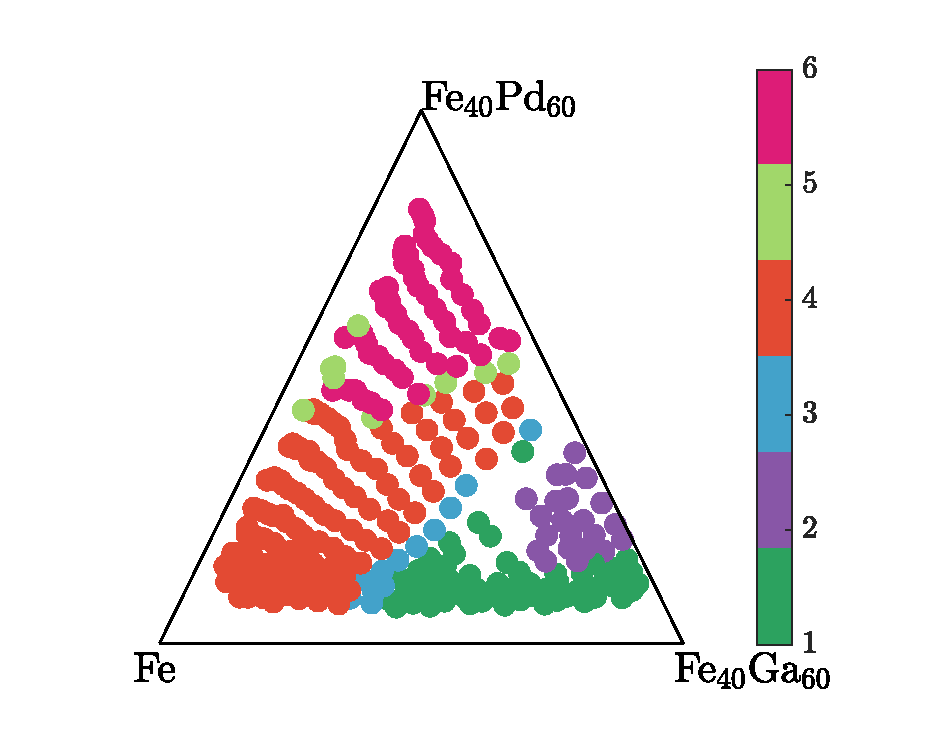
\includegraphics[width=1\textwidth]{Chapter-2/figs/fig5a.eps}
        \caption{Phase diagram reported in \cite{long2007rapid}}
        \label{refFePdGa}
    \end{subfigure}
    \quad
        \begin{subfigure}[b]{0.475\textwidth} 
        \centering 
        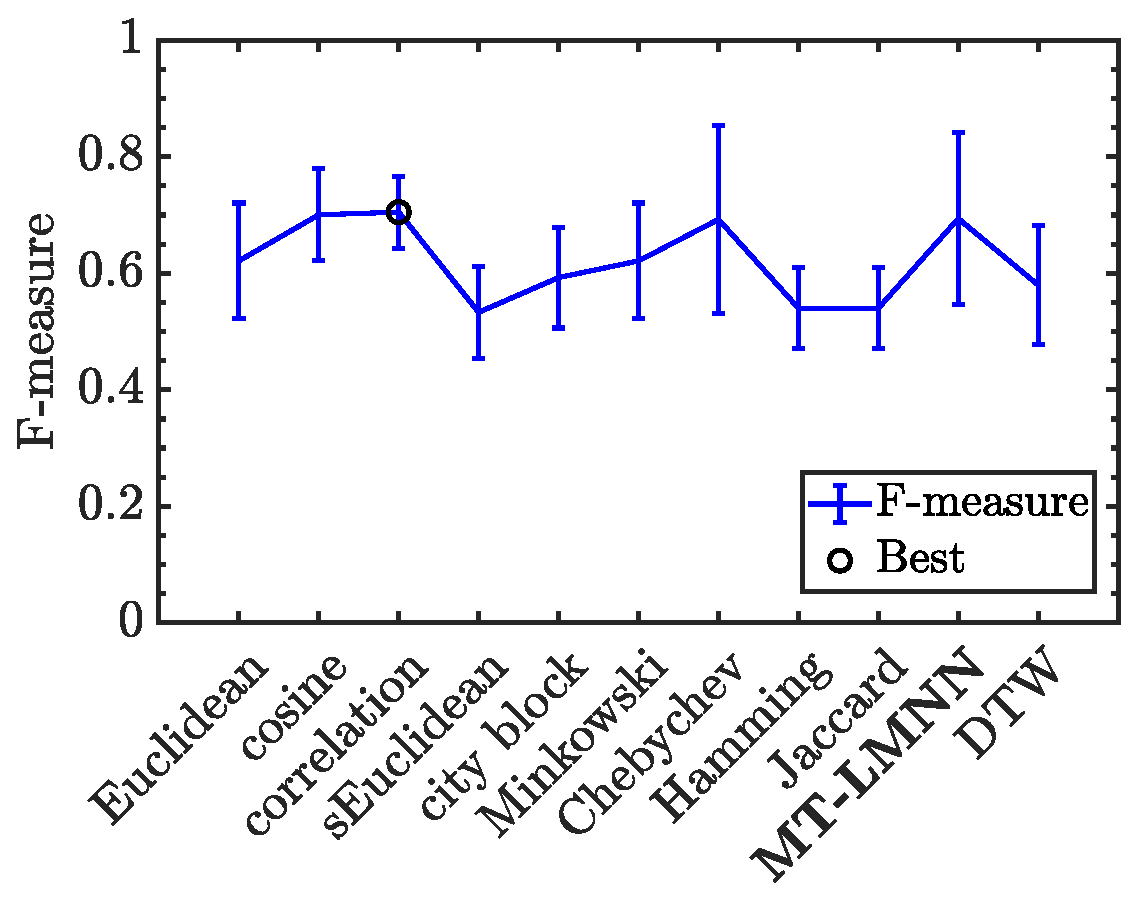
\includegraphics[width=1\textwidth]{Chapter-2/figs/fig5b.eps}
        \caption{F-measure statistics}
        \label{errorsFePdGa}
    \end{subfigure}
    \quad
    \vskip\baselineskip
        \begin{subfigure}[b]{0.475\textwidth} 
        \centering 
        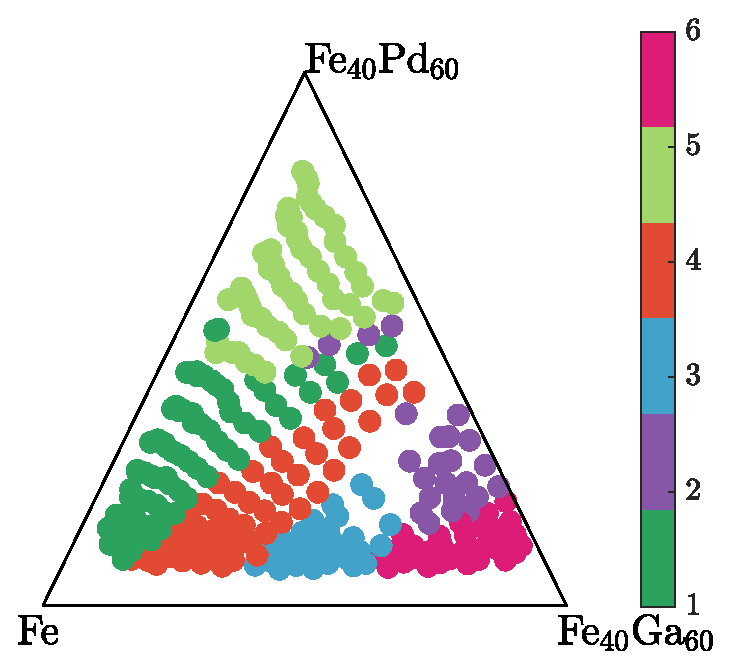
\includegraphics[width=0.8\textwidth]{Chapter-2/figs/fig5c.eps}
        \caption{Phase diagram using correlation}
        \label{FePdGaCorr}
    \end{subfigure}
    \quad
    \begin{subfigure}[b]{0.475\textwidth} 
        \centering 
        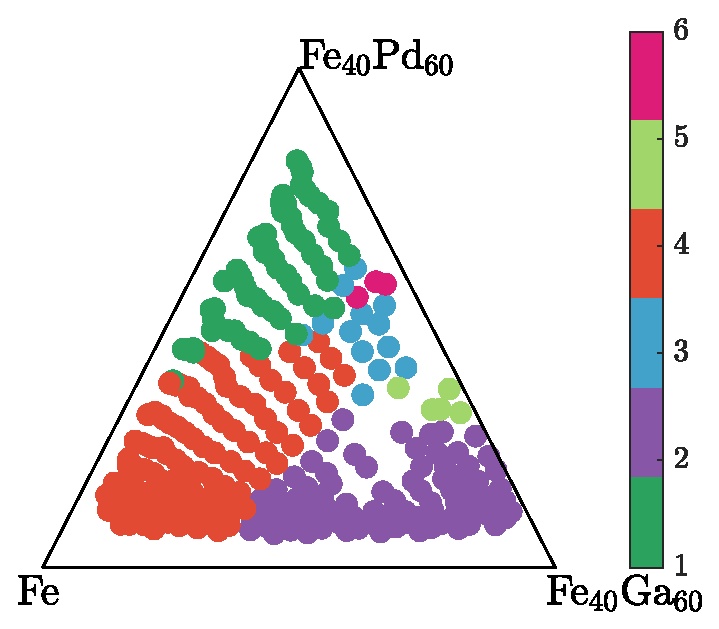
\includegraphics[width=0.8\textwidth]{Chapter-2/figs/fig5d.eps}
        \caption{Phase diagram using MTML}
        \label{FePdGaMLPD}
    \end{subfigure}
\caption{Comparison of phase diagram deduced using various similarity measure. \Cref{FePdGaCorr,FePdGaMLPD} depict the representative phase diagrams (most frequent or stable for among various clustering settings/parameters used for the true number of clusters).}
    \label{FePdGa}
\end{figure}
\section{Conclusions}
In this chapter, we introduced a distance measure learning approach into the data analytics for compositional libraries. 
A metric was learned from the data using the composition information about the design space. 
This is in contrast to the exhaustive search for a suitable distance measure.
Two case studies consisting of model cyclic voltammetry and experimental XRD responses as high-dimensional signals are presented and evaluated using a variety of statistical tests.
We showed that our method has the ability to identify regions in the design space where a systematic variation in design variable gives rise to systematic variation in response. 
Using a model electrochemistry data, we showed that a distance measure learned using our approach is at least as good as the metric chosen using an exhaustive search.
Through various test cases, we have shown that learning a similarity measure using MT-LMNN has the ability to automatically quantify the similarity measure for any given data set. This makes MT-LMNN a better alternative to an exhaustive search of complex and data specific metrics as well as a promising approach for automated distance learning for compositional libraries. 

\chapter{Active knowledge extraction from cyclic voltammetry}\label{chapter3}
Cyclic Voltammetry~(CV) is an electro-chemical characterization technique used in an initial material screening for desired properties and to extract information about electro-chemical reactions.
In some applications, to extract kinetic information of the associated reactions (e.g., rate constants and turn over frequencies), CV curve should have a specific shape (for example an S-shape). 
However, often the settings to obtain such curve are not known \textit{a priori}. 
In this chapter, an active search framework is defined to accelerate identification of settings that enable knowledge extraction from CV experiments.
Towards this goal, a function space representation of CV responses is used in combination with Bayesian Model Selection (BMS) method to efficiently label the response to be either \textit{S-shape} or not \textit{S-shape}. 
Using an active search with BMS oracle, we report a linear target identification in a 6-dimensional design space (comprising of thermodynamic, mass transfer and solution variables as dimensions). 
The framework has the potential to be a powerful virtual screening technique for molecular catalysts, bi-functional fuel cell catalysts etc.


\section{Introduction}
Cyclic Voltammetry~(CV) is an electro-chemical characterization technique that measures current generated under a cyclic voltage load between a initial and final voltages varied at a given rate.
The measured current is a highly non-linear response from various physical phenomenon such as mass transport, kinetics, adsorption etc. 
In principle, it is possible to determine the properties associated with the underlying physical phenomenon. 
However, the property extraction is a non-trivial task. 
In a CV experiment, a steady state current is obtained when all reactions in the mechanism have the same apparent rate constants~\cite{BardFaulkner}. 
This is because the facile reactions in the sequence are held back from their maximum rates by the sluggish reactions called a \textit{rate determining step} that also determines the magnitude of steady state current.   
Extracting rate constants of the rate determining step thus requires the CV curve to be in a S-shape~\cite{costentin2015cyclic, rountree2014evaluation} with a clear steady state current region resolved during measurement. 
Towards this goal, obtaining a S-shaped CV curve requires the experiment to be run with a set of conditions~(e.g, temperature, substrate concentration, scan rate), amenable for S-shape CV curves which are unknown \textit{a priori}.
Moreover, choosing conditions where a given electrochemical system exhibits a S-shaped CV curve is dependent on underlying system of electrochemical reaction(s) which is(are) also unknown for novel materials. 
In the absence of a known mechanism, an exhaustive search over all the possible tunable parameters is performed~\cite{martin2016qualitative} to narrow down the region of interest. 
Such exhaustive strategy comes at a price of a very high computational cost especially in high-dimensional search spaces of multiple complex reaction mechanisms.

As an alternative approach, experts define a figure of merit~(FOM)~\cite{rountree2014evaluation}(a performance measure) as a proxy signature of a physical phenomenon of interest. 
FOM extracted from CV can be also used in material discovery using data-driven methods. 
For example, in~\cite{stein2019functional,li2019application,haber2014high,suram2015generating} different types of FOM have been used for catalyst discovery using data-driven methods.
With FOM defined, the goal is to find a material that produces a response with a FOM that is better than that of known materials.
For instance, in case of a high-throughput exploration for a new catalyst, the overpotential is a common FOM~\cite{norskov2004origin}(or performance measure) used in the combinatorial searches~\cite{suram2015generating}. 
The over-potential can be thought of as the voltage~(beyond the thermodynamic requirement) required to produce a (pre-defined) target current.
This FOM has clear utility to screen for well performing materials, but misses on the main advantage of CV - that is the capability to extract the kinetic information~(such as rate constants~\cite{FOWA}, turn-over frequencies~\cite{TOF,FOWA2}).

Given the time and financial constraints, an active learning method~\cite{jiang2018efficient,RGActiveIntro, GardnerALIntro} is proposed to accelerate the process of extracting kinetic information from CV curves. 
Rather than relying on the selection of figure of merit, a function space representation of our target~(S-shaped) and non-target~(everything else) CV responses is used in the Bayesian Model Selection (BMS) for automatic classification. 
We encode prior knowledge of target and non-target CV responses using the basis functions of a Gaussian processes~(\(\mathcal{GP}\)) function space.
\(\mathcal{GP}\) have been previously used to infer the kinetic parameters~\cite{gavaghan2018use,robinson2018separating} of a CV response by using a maximum likelihood estimate and \(\mathcal{GP}\) regression. 
In another work ~\cite{li2019application}, a Bayesian approach is used to search for an approximate rate constant when the reaction mechanism is known. 
In this work, however, \(\mathcal{GP}\) is used as a data representation model to distinguish S-shaped CV curves from other types of continuous CV curves. 
Once a S-shaped CV curve is collected, the foot-of-the-wave analysis~(FOWA)~\cite{FOWA} can be used to extract the rate constant of a rate determining step. 
When combined together with FOWA, the proposed approach can be a robust technique that does not require any knowledge of the actual reaction mechanism.

In this chapter, we focus on S-shaped CV responses due to their utility for:~a) extracting kinetic information~\cite{costentin2015cyclic, rountree2014evaluation}--using the foot of the wave analysis~\cite{FOWA} that can only be applied to a S-shaped CV curve.~b) screening for bi-functional catalysts -- materials that produce CV curves similar to S-shape in two different voltage sweep ranges~\cite{bradley2019reversible, jung2016optimizing}. 
While the two applications are different, they can be approached under a common framework of active search to find S-shaped CV curves within the combinatorial space. 


The rest of the chapter is organized as follows: (i)~First  Bayesian active learning framework is introduced with a general probabilistic model. Then a connection is established between collected data at observed locations with the oracle used to classify and update the decision model used for active learning. (ii)~Bayesian Model Selection~(BMS) procedure is then introduced to compute a classification preference for targets and non-targets based on collected data and a set of parametric models. (iii)~a \(\mathcal{GP}\) model is introduced from a function space representation point of view to be used as a parametric model in BMS.  (iv)~The methodology is then applied to a search space of a simple EC mechanism to demonstrate the application of the BMS oracle to classify CV responses in order of its S-shape. (v)~Finally, the BMS oracle is used in active search to address the challenges in knowledge extraction, virtual screening of materials for electrochemical applications using cyclic voltammetry.
\section{Methods}
The goal is to identify the measurement settings from which one can extract kinetic information captured in a CV response.
Towards this goal, we seek to identify measurement conditions for which an S-shape CV curve is collected by our oracle. 
We use an active learning technique summarized in~\Cref{fig:workflow} to accelerate the search for measurement settings within fixed computational budget. 
The active learning approach involves iterative collection of data points from a search space \(\mathcal{S}\).
The process starts with a small set of observed data \(D=(\textbf{S},\textbf{Y})\) where \(\textbf{S}\in\mathcal{S}\) are the observed locations and \(\textbf{Y}\in\{-1,1\}\) are corresponding labels. 
In each iteration, the algorithm collects data and incrementally updates the decision model \(p(y=+1|D)\) it aims to learn with \(y\) representing a label.
A user-defined selector~(or policy) identifies a~(or a batch of) candidate location(s) in the search space for observing the responses.
The policy typically maximizes a utility function given the decision model. 
For example, given \(D\), we can define a policy using a utility function that simply counts number of targets in the dataset \(u(\textbf{S})=\sum\limits_{s_i\in \textbf{S}, y_i \in \textbf{Y}} [y_i=+1]\). 
A policy can be defined to select more targets to be added to the data pool \(D\) using: 
\begin{equation}
    s^* = \argmax_s \mathbb{E}\left[ u(\mathcal{S} \setminus \textbf{S} | D )\right] 
    \label{eq:policy}
\end{equation}
Given a location \(s^* \in\mathcal{S}\), the corresponding experiment is performed and a response is collected. 
In this chapter, a CV response curve is collected from a CV curve simulator and the response is then passed onto an oracle. 
Oracle labels the response to be either a target or non-target~(for example in~\Cref{fig:workflow}, we show a non-target like CV shape which will be  assigned \(y^*=-1\) as a label). 
The next step is to augment \(D\) using the data collected in the current iteration i.e. \(D^* = D\cup (s^*,y^*) \). 
The decision model is then updated with \(D^*\). 
This process is repeated until computational budget--defined in terms of total number of label queries or equivalently number of simulations--is exhausted.
As an oracle we use a Bayesian Model Selection (BMS) that operates on two models \(\mathcal{M}_1, \mathcal{M}_2\) referred to as null model~(representing a typical CV curve) and target model~(representing an S-shaped CV curve), respectively.
Moreover, we use a variation of active learning called active search~\cite{garnett2012bayesian} which maximizes the number of targets found in contrast to traditional active learning where the selector is defined with a goal to closely approximate \(p(y=+1\vert D )\).


\begin{figure}[h]
    \centering
    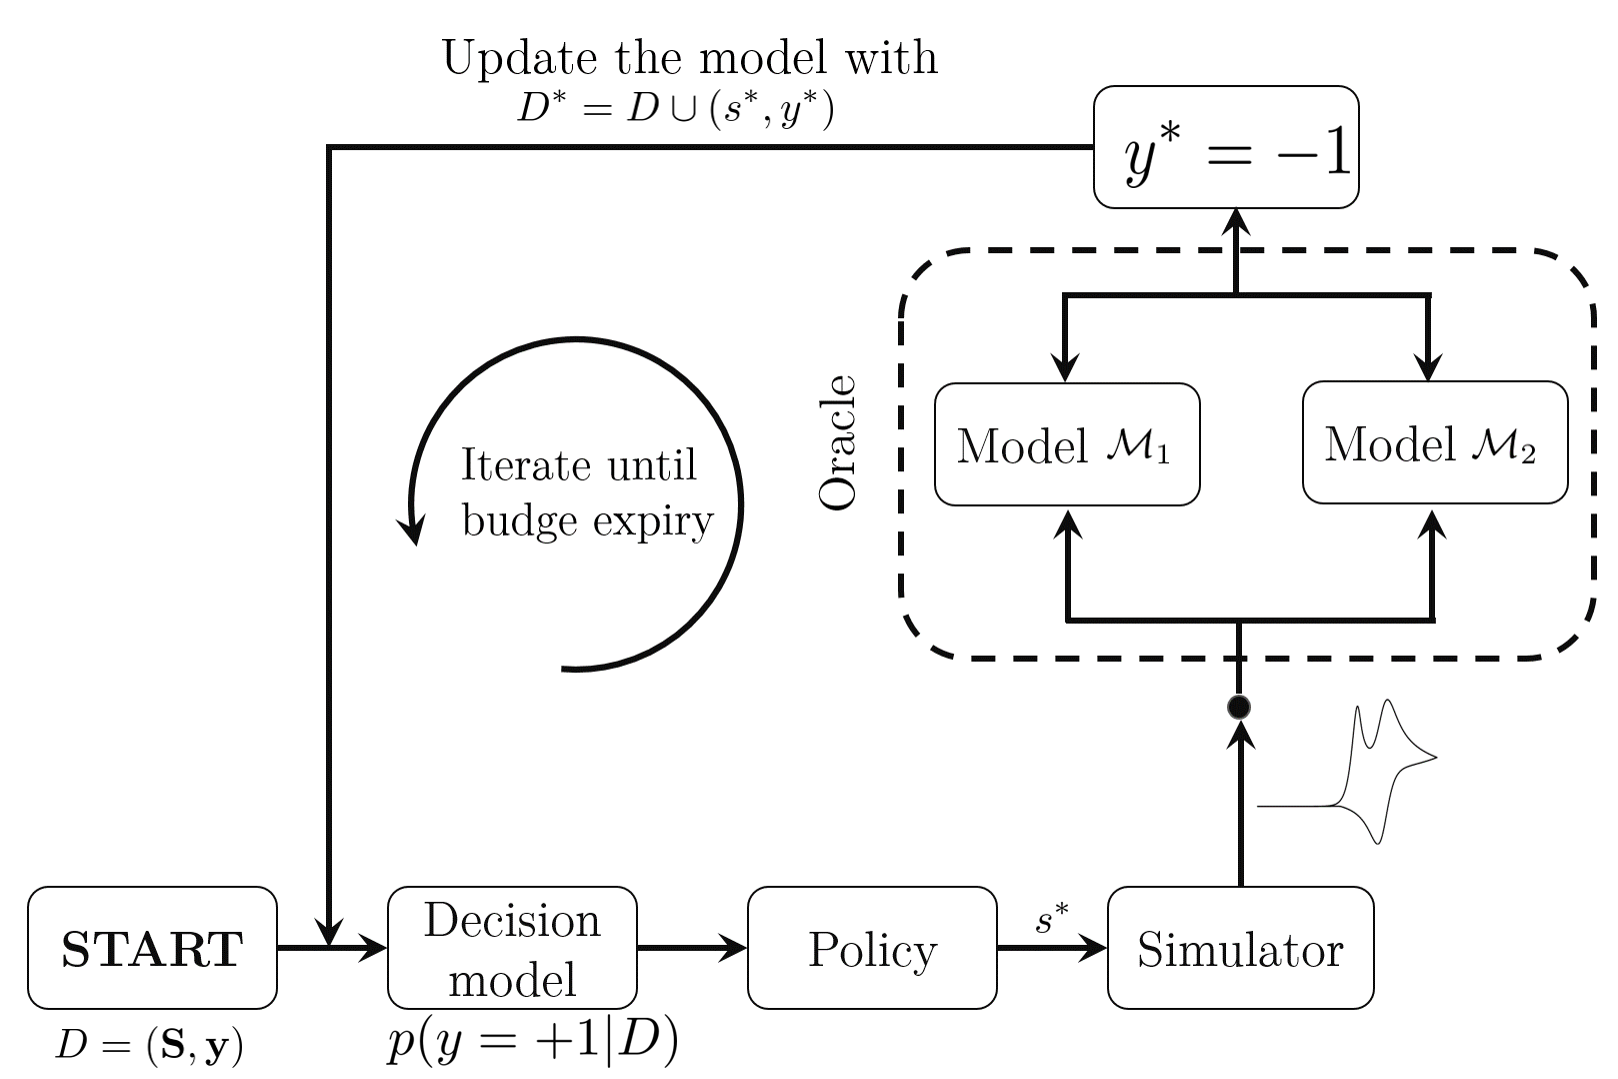
\includegraphics[width=0.75\linewidth]{Chapter-3/figures/workflow_gpcv.png}
    \caption{Active learning framework as a flowchart. Active learning iterations start with a few labelled data points in the search space \(\mathcal{S}\). We stop collecting data when we have selected a pre-defined number (called budget) of locations for updating our decision (or belief) model.}
    \label{fig:workflow}
\end{figure}

\section{Bayesian Model Selection}
The BMS is a tool to identify a preferred model from a family of parametric probability distributions, each of which can explain the observed data with differing degrees of fidelity. 
Using a supervised learning procedure that compares an input \(\textbf{X}\) and output \(\textbf{y}\), we compute a model posterior using Bayes rule to select the model that best explains the observed data \(\mathcal{D}=(\textbf{X},\textbf{y})\). 

Here, given the observed data \(\mathcal{D}=(\textbf{X}, \textbf{y})\), we compute probability that the data is sampled from any given model encoding our prior information. 
Computed posterior probabilities will be used as a score to differentiate whether the collected response (for example, a CV response at any input location in the search space of materials) is a target~(with higher probability for the corresponding target model) or not. 
In this chapter, we use both BMS and active learning in a related but different context. 
BMS is used with observed data encoding a single CV curve while active learning is used in the search space with their corresponding binary labels~(i.e. a target or not) as observed data. 
Moreover, BMS is used as an oracle for the active learning task with models \(\mathcal{M}_j\) as \(\mathcal{GP}\).

For each model \(\mathcal{M}\) with a parameter index \(\theta\)-- a concatenated vector of hyper-parameters-- we first compute model evidence \(p(\textbf{y}\vert \textbf{X},\mathcal{M})\) on the observed data \(\mathcal{D}=(\textbf{X}, \textbf{y})\):
\begin{equation}
    p(\textbf{y}\vert \textbf{X},\mathcal{M}) = \int p(\textbf{y}\vert \textbf{X},\theta,\mathcal{M})p(\theta\vert \mathcal{M}) \diff \theta
\label{eq:evidM}
\end{equation}
where \(p(\textbf{y}\vert \textbf{X},\theta,\mathcal{M})\) is probability of obtaining outputs \(\textbf{y}\) given input data \(\textbf{X}\) and a model \(\mathcal{M}\). \(p(\theta\vert \mathcal{M})\) represents distribution of parameter \(\theta\) for any given model \(\mathcal{M}\).

To understand which model to prefer from a finite set of models  \(\bigl\{\mathcal{M}_i\bigr\}_{i=1}^n\), we apply the Bayes rule to compute the posterior probability of each model \(\mathcal{M}_{j}(j\in\{1,2,..n\})\) given data \(\mathcal{D}\) using the posterior of~\Cref{eq:evidM}: 
\begin{equation}
    p(\mathcal{M}_j\vert \mathcal{D}) = \frac{p(\textbf{y}\vert \textbf{X},\mathcal{M}_j)p(\mathcal{M})}{p(\textbf{y},\textbf{X})}
    \label{eq:postM}
\end{equation}
where \(p(\mathcal{M})\) represents a prior over the finite set of models that is typically taken to be uniform i.e. no prior preference to any single model. 
One common approach is to use logarithm of the probability which can be interpreted as the information content of a probability model given data. 
Taking the logarithm of~\Cref{eq:postM}, we get the following~(See Supplementary Information): 
\begin{equation}
    \log p(\mathcal{M}_j\vert \mathcal{D}) = -\log \left [ 1+\sum_{i\neq j}^{n} \frac{p(\textbf{y}\vert \textbf{X},\mathcal{M}_i)}{p(\textbf{y}\vert \textbf{X},\mathcal{M}_j)}\right]
\label{eq:logPostM}
\end{equation}





\subsection{\(\mathcal{GP}\) Models for Catalytic Responses}
A \(\mathcal{GP}\) is a distribution over smooth latent functions \(g: \mathcal{X} \rightarrow \mathbb{R}\). 
Assuming the observation model \(p(y\vert g)\) is known, the standard approach is to use non-parametric Bayesian approach by placing a \(\mathcal{GP}\) distribution over \(g\), i.e. \(p(g)=\mathcal{GP}\big(\mu(x),k(x,x')\big)\). 
Here \(\mu(x):\mathcal{X}\rightarrow \mathbb{R}\) is a mean function and \(k(x,x'):\mathcal{X}\times\mathcal{X}\rightarrow \mathbb{R}\) is a covariance function. 
A function-space viewpoint provides an intuitive explanation of \(\mathcal{GP}\) as vector space of functions in a chosen (potentially non-linear) feature space which \(\phi(x)\) as a basis. 
In the function space representation, the observation model plays the role of weights \(W\) with function \(g\) represented using \(g(x) = \phi(x)^{\top}W\). 
It can be shown~(see Supplementary Information) that \(\phi(x)\) can be implicitly defined using the covariance function \(k(x,x')\) between pair of inputs \(x,x'\in\mathcal{X}\) and a mean function \(\mu(x)\) of \(W\)~\footnote{for this reason we use \(k(x,x')\) and basis function of \(\mathcal{GP}\) interchangeably in this paper}. 
The mean function \(\mu\) encodes an average behavior of the function \(g\). 
The covariance function \(k(x,x')\) encodes the correlations between outputs \(g(x), g(x')\) for any given pair of input points~(\(x,x'\)). 
In this chapter, the concatenated vector of the parameters \(\mu(x)\) and \(k(x,x')\) is denoted as \(\theta\).
Once we select a \(\mathcal{GP}\) encoding our prior beliefs, we use Bayes rule to update our posterior \(p(g\vert \mathcal{D})\) conditioned on observed data \(\mathcal{D}=(\textbf{X},\textbf{y})\) where \(\textbf{y}\) are the discrete evaluations of function \(g\) at inputs \(\textbf{X}\). 
For more information on \(\mathcal{GP}\), readers are referred to~\cite{williams2006gaussian}.

A typical response from a cyclic voltammetry experiment is represented as a function \(I(t,v)\) with \(I\) being the current response collected at a time (\(t\)) for a time dependent applied voltage \(v=V(t)\). 
The voltage load \(V(t)\) is typically chosen to be linear and the voltammetry is often referred as direct current voltammetry~\cite{li2019application}.
Classification of a CV into an S-shape (or not S-shape) can be looked at as determining a model evidence of a function defined by CV curve \( (v,t) \mapsto I\) under a \(\mathcal{GP}\) function space with observed data \(\mathcal{D}\) given by the discrete CV curve \(\textbf{X} = I, \textbf{y}=(v,t)\). 
The covariance of a CV curve gives rise to the basis functions in the \(\mathcal{GP}\) space and the time-voltage grid becomes the input space where the function is evaluated.
For any given CV curve, its representation in the \(\mathcal{GP}\) function space  is obtained by finding a \(\theta\) that maximize the posterior probability \(p(\textbf{X} = I|\textbf{y}=(v,t))\)~\footnote{we use the \textit{maximum a posteriori} or MAP estimation}.
The \(\mathcal{GP}\) model is chosen with a \textit{non-stationary} covariance as a target model~\(\mathcal{M}_2\). 
It follows from the reproducing kernel Hilbert space~(RKHS) theorem~(Ch 12.4 in \cite{mathML}) that any smooth function can be represented using a kernel or a covariance function.
Thus for the null model~(\(\mathcal{M}_1\)), it is sufficient to use a \(\mathcal{GP}\) with smoothness controllable covariance function. 
A brief overview of the covariance functions selected as basis functions is described below.
For both models \(\mathcal{M}_1\) and \(\mathcal{M}_2\), the mean function is chosen to be \(\mu(x)=0 \) as we normalize the response curves \(I(v,t)\) to be with in \((0,1)\) and expect the covariance function to determine the shape of the CV curve. 

\subsubsection{Squared Exponential Covariance}
The commonly known \textit{squared exponential kernel}~(in~\Cref{eq:covSEard} and~\Cref{fig:covSEard}) is used as a covariance model for \(\mathcal{M}_1\) where the resulting feature map \(\phi(x)\) forms a basis for functions that are smooth and stationary.
\begin{equation}
    k(x,x')=\sigma_f^2 \exp((x-x')^{\top}\Lambda^{-1}(x-x'))
    \label{eq:covSEard}
\end{equation}
In~\Cref{eq:covSEard}, \(\sigma_f\) is scaling parameter, and \(\Lambda\) is a diagonal matrix with each entry as a length scale for the corresponding dimension of \(x,x'\in \mathcal{X}\). 
The left panel of \Cref{fig:covSEard} depicts five samples drawn at random from the \(\mathcal{GP}\) with the covariance in~\Cref{eq:covSEard}.% The input to the function \(g\) s \(x\) and real valued outputs as \(g(x)\). 
The right panel of the same figure depicts the covariance function visualized on a uniform grid of \(\mathcal{X}\times\mathcal{X}\) as contours. 
From~\Cref{fig:covSEard}, it can be seen that the covariance is stronger~(\(\approx 1\)) between inputs with Euclidean norm~(i.e. distance) less than a length scale controlled by the parameter \(\Lambda\).

\begin{figure}[h]
    \centering
    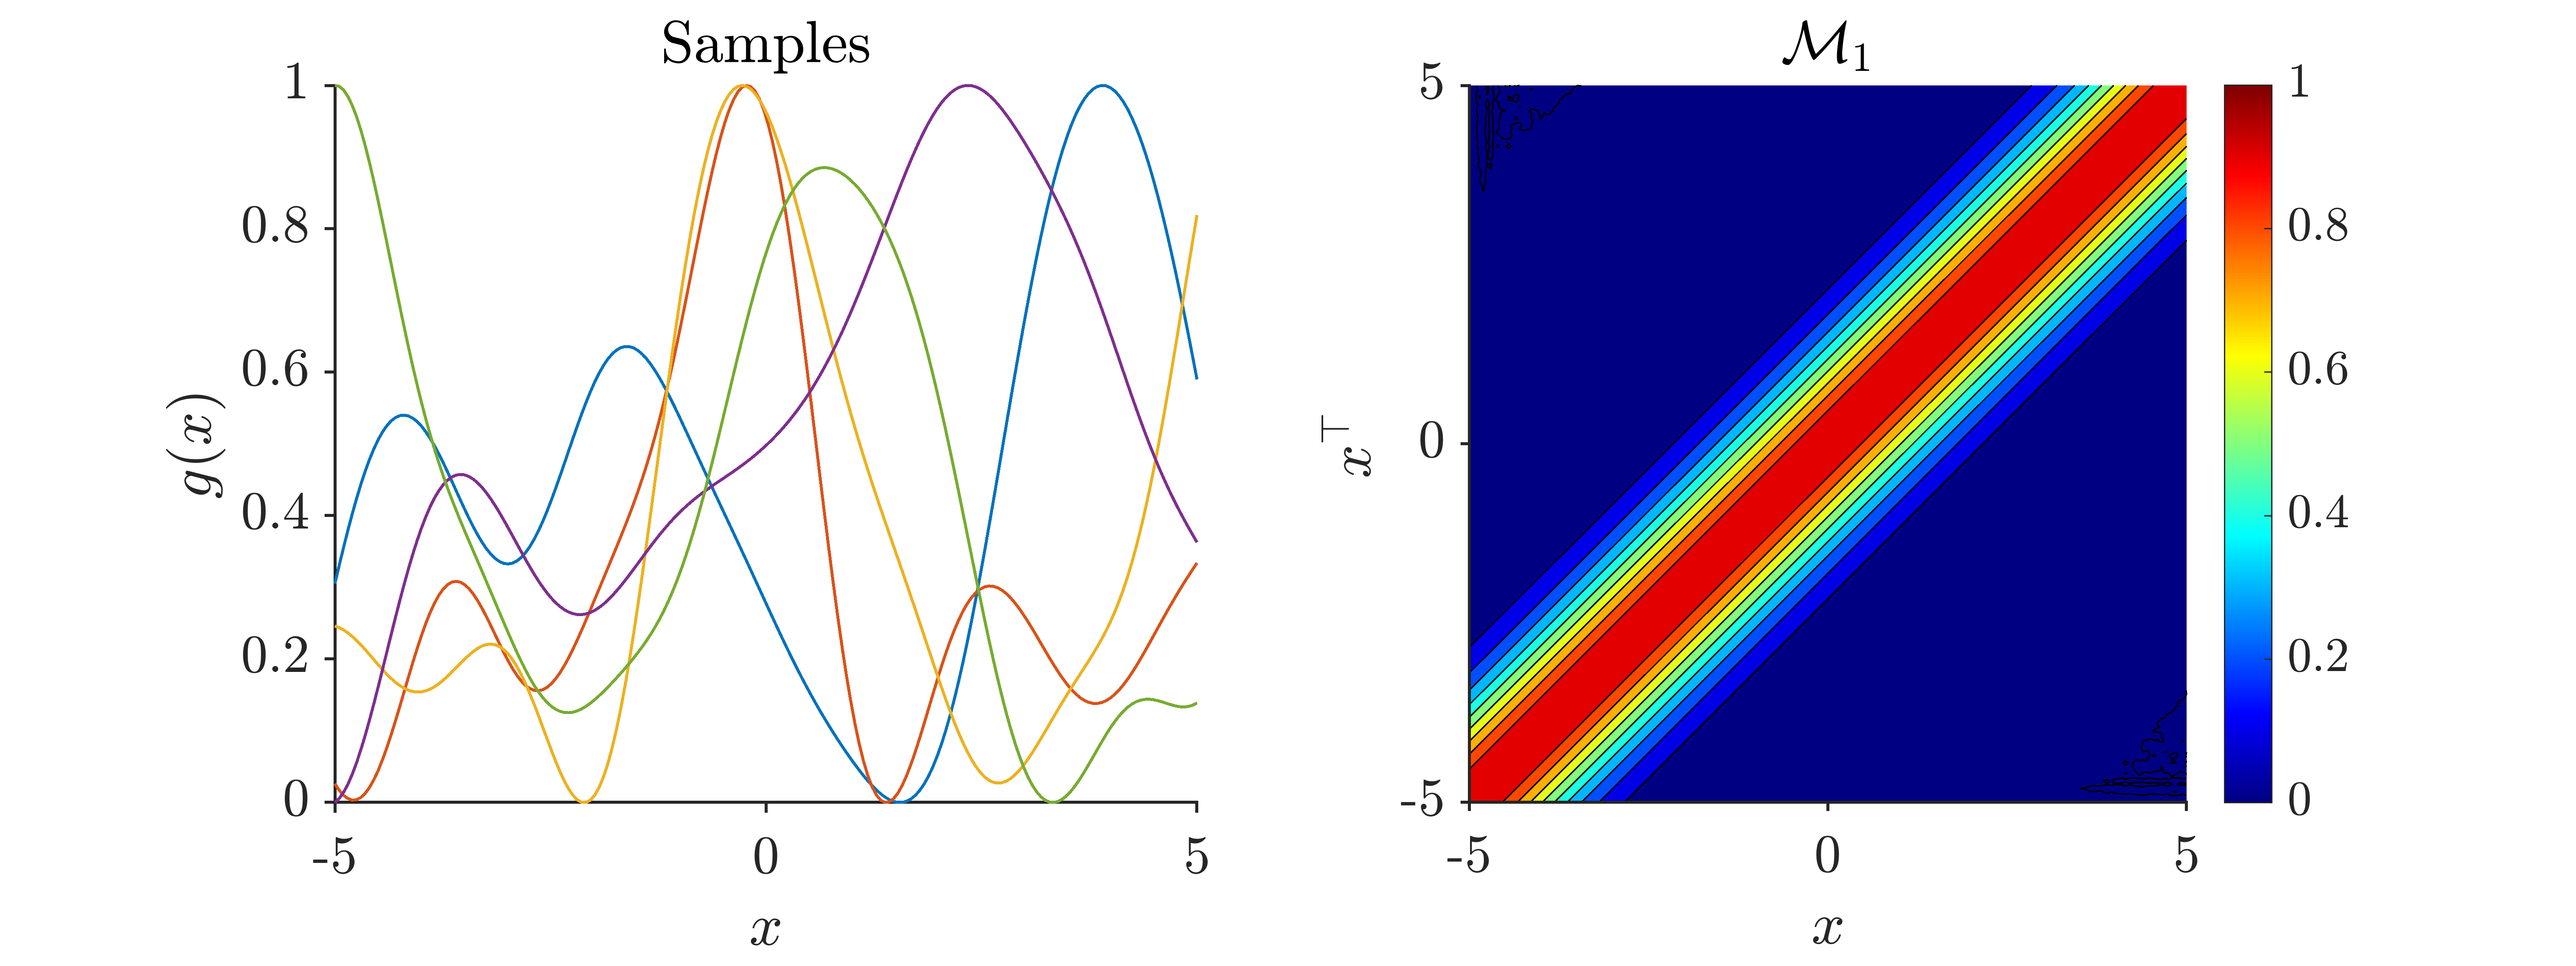
\includegraphics[scale=0.5]{Chapter-3/figures/Model1.png}
    \caption{A pictorial representation of~\Cref{eq:covSEard}. Left panel: five samples drawn at random from the \(\mathcal{GP}\) built using~\Cref{eq:covSEard}, captures the smooth and locally correlated nature of the \(\mathcal{GP}\). Right panel: a contour plot depicting correlations between outputs of one-dimensional vectors \(x,x' \in \mathcal{X}\). Color code represents the covariance \(k(x,x')\) with red representing high covariance i.e. output values \(g(x), g(x')\) are highly correlated and vice-versa. }
    \label{fig:covSEard}
\end{figure}

\subsubsection{Neural Network Covariance}
The target model uses neural network covariance kernel to build a \(\mathcal{GP}\) function space representation referred as model~\(\mathcal{M}_2\)(shown in~\Cref{eq:covNNone} and~\Cref{fig:covNNone}).
The S-shape responses have a non-stationary covariance and hence a covariance that is effective in handling rapidly changing signals would be a good choice. 

\begin{align}
        k(x,x') &= \sigma_f^2 \sin^{-1}\left({\frac{x^{\top}\Lambda^{-2}x'}{\sqrt{h(x)h(x')}}}\right) \label{eq:covNNone}\\
        h(x) &= 1+x^{\top}\Lambda^{-2}x \nonumber
\end{align}
In~\Cref{eq:covNNone}, \(\sigma_f\) is scaling parameter, and \(\Lambda\) is a diagonal matrix with each entry as a length scale.
\Cref{fig:covNNone} is analogues to~\Cref{fig:covSEard} and it can be seen that the covariance is high~(\(\approx 1\)) in two blocks of input locations that are separated by a completely uncorrelated input locations~(covariance \(\approx 0\)). 
This is in contrast to \(\mathcal{M}_1\) where the covariance is determined by some form of distance between input points. 
\begin{figure}[h]
    \centering
    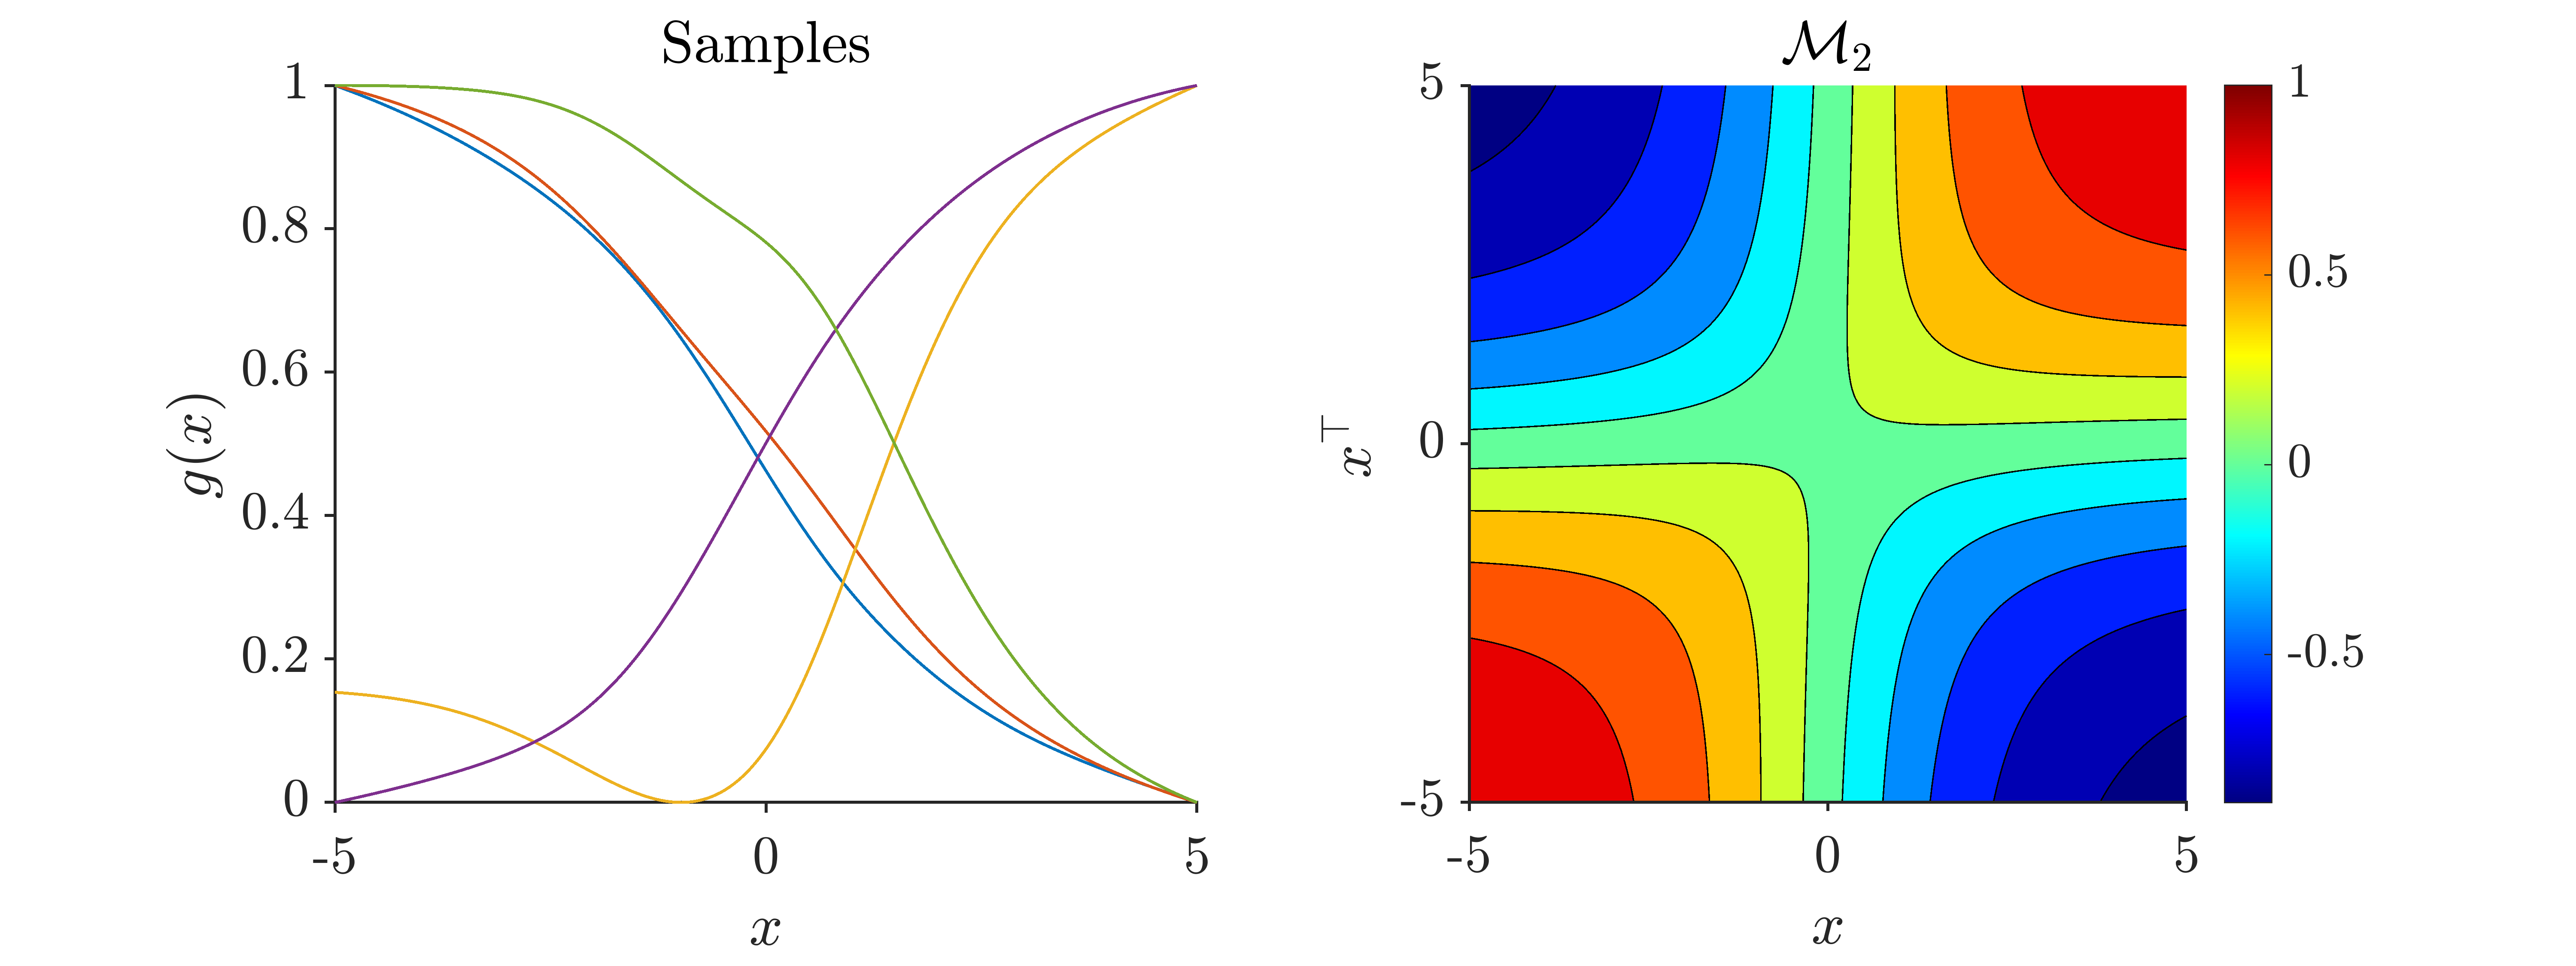
\includegraphics[scale=0.5]{Chapter-3/figures/Model2.png}
    \caption{A pictorial representation of~\Cref{eq:covNNone}. Left panel: five samples drawn at random from the \(\mathcal{GP}\) built using~\Cref{eq:covNNone}, captures the non-stationary nature nature of the \(\mathcal{GP}\) signified by constant values and sharp rises in the response values. Right panel: a contour plot of covariance between two one-dimensional vectors \(x,x' \in \textbf{X}\) as inputs. A positive value for \(k(x,x')\) signifies that output values \(g(x), g(x')\) are highly correlated and vice-versa. }
    \label{fig:covNNone}
\end{figure}



\section{Results}
To demonstrate the application of active search for S-shaped CV curves, we choose to simulate CV curves of a classic EC-mechanism, that consists of two reactions: E and C (\Cref{E} and \Cref{C}) corresponding to one electron transfer reaction (E) and one chemical reaction (C), respectively. 
EC-mechanism is selected as it is a well studied mechanism~\cite{rountree2014evaluation, costentin2015cyclic} that produces a variety of CV shapes thus serves as a good test case for the oracle described earlier. 
In this work, we use the MECSim simulator~\cite{MECSim} to generate CV curves on demand. 

\subsection{Data generation}\label{sec:data}
The EC mechanism is a two step reaction comprising of an electron transfer~\Cref{E} followed by a chemical reaction in~\Cref{C}. 
\begin{chequation}
\begin{align}
    &\ce{P + e <=> Q} \label{E}\\
    &\ce{Q + A -> P } \label{C}
\end{align}
\end{chequation} 
Electro-chemical kinetics of the EC mechanism can be modeled and solved using governing partial differential equations~\cite{saveant1984homogeneous}. 
In this section, we are interested in modeling the (micro)kinetics of species (and electron) that contributes to current generation under cyclic voltage sweep at a given sweeping rate.

Towards this goal, the transport of the three species (P, Q, A) in the solution is modelled using Fick's second law of diffusion with a source term corresponding to the heterogeneous reactions:
\begin{align}
    \pdv{C_P}{t} &= D_{\text{diff}}\pdv[2]{C_P}{u} + k_{s}C_{Q}C_{A} \nonumber\\
    \pdv{C_Q}{t} &= D_{\text{diff}}\pdv[2]{C_Q}{u} - k_{s}C_{Q}C_{A} \nonumber\\
    \pdv{C_A}{t} &= D_{\text{diff}}\pdv[2]{C_A}{u} - k_{s}C_{Q}C_{A} \label{eq:fickslaws}
\end{align}
with the boundary conditions defined as follows:
\begin{align}
    t&=0, \forall u &  &C_P = C^0_{P}, C_A = C^0_{A}, C_Q = C^0_{Q} \nonumber \\
    t&>0, u\rightarrow \infty &  &C_P = C^0_{P}, C_A = C^0_{A}, C_Q = C^0_{Q}  \nonumber\\
    t&>0, \forall u &  &\pdv{C_A}{u}=0; \pdv{C_P}{u}+\pdv{C_Q}{u}=0; C_P/C_Q = \exp(\frac{F}{RT}(V-E^0)) \label{eq:bcs}
\end{align}
In~\Cref{eq:fickslaws,eq:bcs} the formal reversible potential of electron transfer reaction~\cref{E} is \(E^0\), the  concentration of catalyst P is \(C_P\), specie Q is \(C_Q\) and substrate A is \(C_A\). \(D_{\text{diff}}\) is a common diffusion coefficient for all species and \(k_{s}\) is the rate constant of the forward reaction in~\Cref{C}. 
The spatial domain is denoted as \(u\) starting from the working electrode~(i.e. \(u=0\)) assuming a semi-infinite domain. The time scale of the simulation is denoted as \(t\). Initial concentrations~(i.e. at \(t=0\)) are denoted with a superscript 0. \(V\) represents the time varying applied voltage. 
For a cyclic voltage sweep between voltages \(V_i, V_f\) at a rate of \(\nu~V/s\) we get~\Cref{eq:voltage_scan} for V~(\(T_s\) is switching time).
\begin{align}\label{eq:voltage_scan}
    V(t) = 
    \begin{cases}
        V_i + \nu t & 0<t<T_s\\
        V_f - \nu t & T<t<2T_s
    \end{cases}
\end{align}
Digital simulation of system of partial differential equations in~\Cref{eq:fickslaws,eq:bcs} is performed to determine spatio-temporal concentration profiles of species P, Q, A. 
The Faradaic current observed during the cyclic voltage load is computed using~\Cref{eq:current} following the Butler-Volmer model for heterogeneous electron transfer at the electrode surface.
\begin{align}\label{eq:current}
    i(t,v) = FA_{\text{surf}}k^0\left[C_Q\exp(\frac{\alpha F}{RT}(V-E^0)) - C_P\exp(\frac{(1-\alpha)F}{RT}(V-E^0))\right]
\end{align}
In~\Cref{eq:current}, \(F\) is Faraday's constant, \(A_{\text{surf}}\) is surface area of electrode~( \(=1~cm^2\)), \(R\) is universal gas constant, \(T\) is room temperature.
\(k^0\) is heterogeneous electron transfer rate constant and \(\alpha\) is a symmetric charge transfer coefficient~(=0.5).
    
We use the freeware software MECSim~\cite{kennedy2015monash,MECSim} to digitally simulate the cyclic voltammetry response in the voltage range of \([-0.5V,0.5V]\). 
Along with the parameters used in~\Cref{eq:fickslaws,eq:bcs}, MECSim can also simulate the effects of an uncompensated resistance (\(R_u\)), double layer capacitance (\(C_{dl}\)) which are not used in this example case study. 
We form a 6-dimensional design search space using \(C_P^0, C^A_0, k_{s}, k^0, \nu, E^0\) and set the values of \(R_u = 0, C_{dl} = 0, \alpha=0.5, D=1\times10^{-5}\). 
\Cref{tab:search_space} lists the combinatorial space defined with six design variables (dimensions of search space) and number of samples along the dimension used to create an exhaustive search grid of tunable settings.
After excluding responses from a diverging simulation arising from a combination of non-physical parameters for MECSim~\footnote{see MECSim documentation for known limitations} we get a total of \(\approx 17\times10^3\) CV curves in our database. 
\begin{table}[h]
\centering
\begin{tabular}{|c|c|c|}
\hline
Parameter & range & number of levels per dimension \\  \hline
\(\log C_P^0 \) &[-2,3] & 5\\ \hline
\(\log C_A^0 \) &[-2,3] & 5\\ \hline
\( E^0 \) &[-0.4,0.4] & 5\\ \hline
\(\log k_{s} \) &[-1,6] & 5\\ \hline
\(\log k^0 \) &[-1,6] & 5\\ \hline
\(\log \nu \) &[-2,4] & 6\\ \hline
\end{tabular}
     \caption{Combinatorial space used to generate CV responses in EC mechanism along with number of levels used in the exhaustive search.}
     \label{tab:search_space}
 \end{table}
 


\subsection{Using BMS as an oracle to identify S-shaped CV curves}
The application of the BMS oracle to label the CV responses as target, if they are of S-shape, and as non-targets otherwise is demonstrated in this section. 
The proposed BMS oracle is used to label the CV responses and couple it with standard active search techniques to find our "targets" within a given budget of label queries (equivalently number of queries to the simulator). 
To accommodate for the high-throughput search running a batch of experiments at a time, we run the active search using both sequential selection of query locations~(batch size \(b=1\)) and a batch selection~(\(b=100\)). 
We use the  design space in~\Cref{tab:search_space} and aim to find as many targets as possible in the resulting combinatorial design space~\(\mathcal{S}\) of six parameters (dimension of \(\mathcal{S}\)). 

To demonstrate the efficacy of the proposed methods, we first pre-compute labels for a set of ten CV curves in \(\mathcal{S}\) of varying shape.
\Cref{fig:repbmsscores} depicts the chosen CV curves ordered based on model posterior~(\Cref{eq:logPostM}) percentile rank.
Notably, the highest scored CV curves have the S-shape which are of interest in this work.
From~\Cref{fig:repbmsscores}, it can be noted that BMS assigned the highest score to CV curves where the forward and backward sweeps overlap exactly i.e. no hysteresis or capacitive behavior~(highlighted using a red box). 
On the other spectrum, the oracle labels several types of CV curves with low scores.  

The good performance of BMS in this study can be attributed to its inherent ability to handle Gaussian noise, which is also of practical interest for cyclic voltammetry responses~\cite{gavaghan2018use}. 
For comparison, we studied two other oracles to rank a CV curve based on their S-shape characteristics using point-wise comparison: a)~\textit{similarity score} that uses a generic approach of computing the Euclidean norm between a given CV curve and user defined reference S-shape; and b) \textit{FOWA score} that is physics inspired and defined as the \(R^2\)-value for any CV curve in Foot of The Wave Analysis~(FOWA) coordinate space~(a perfect symmetric S-shaped CV curve has \(R^2=1\)). 
% We discuss more details on (a,b) in Supplementary Information. 
\begin{figure}[h]
    \centering
    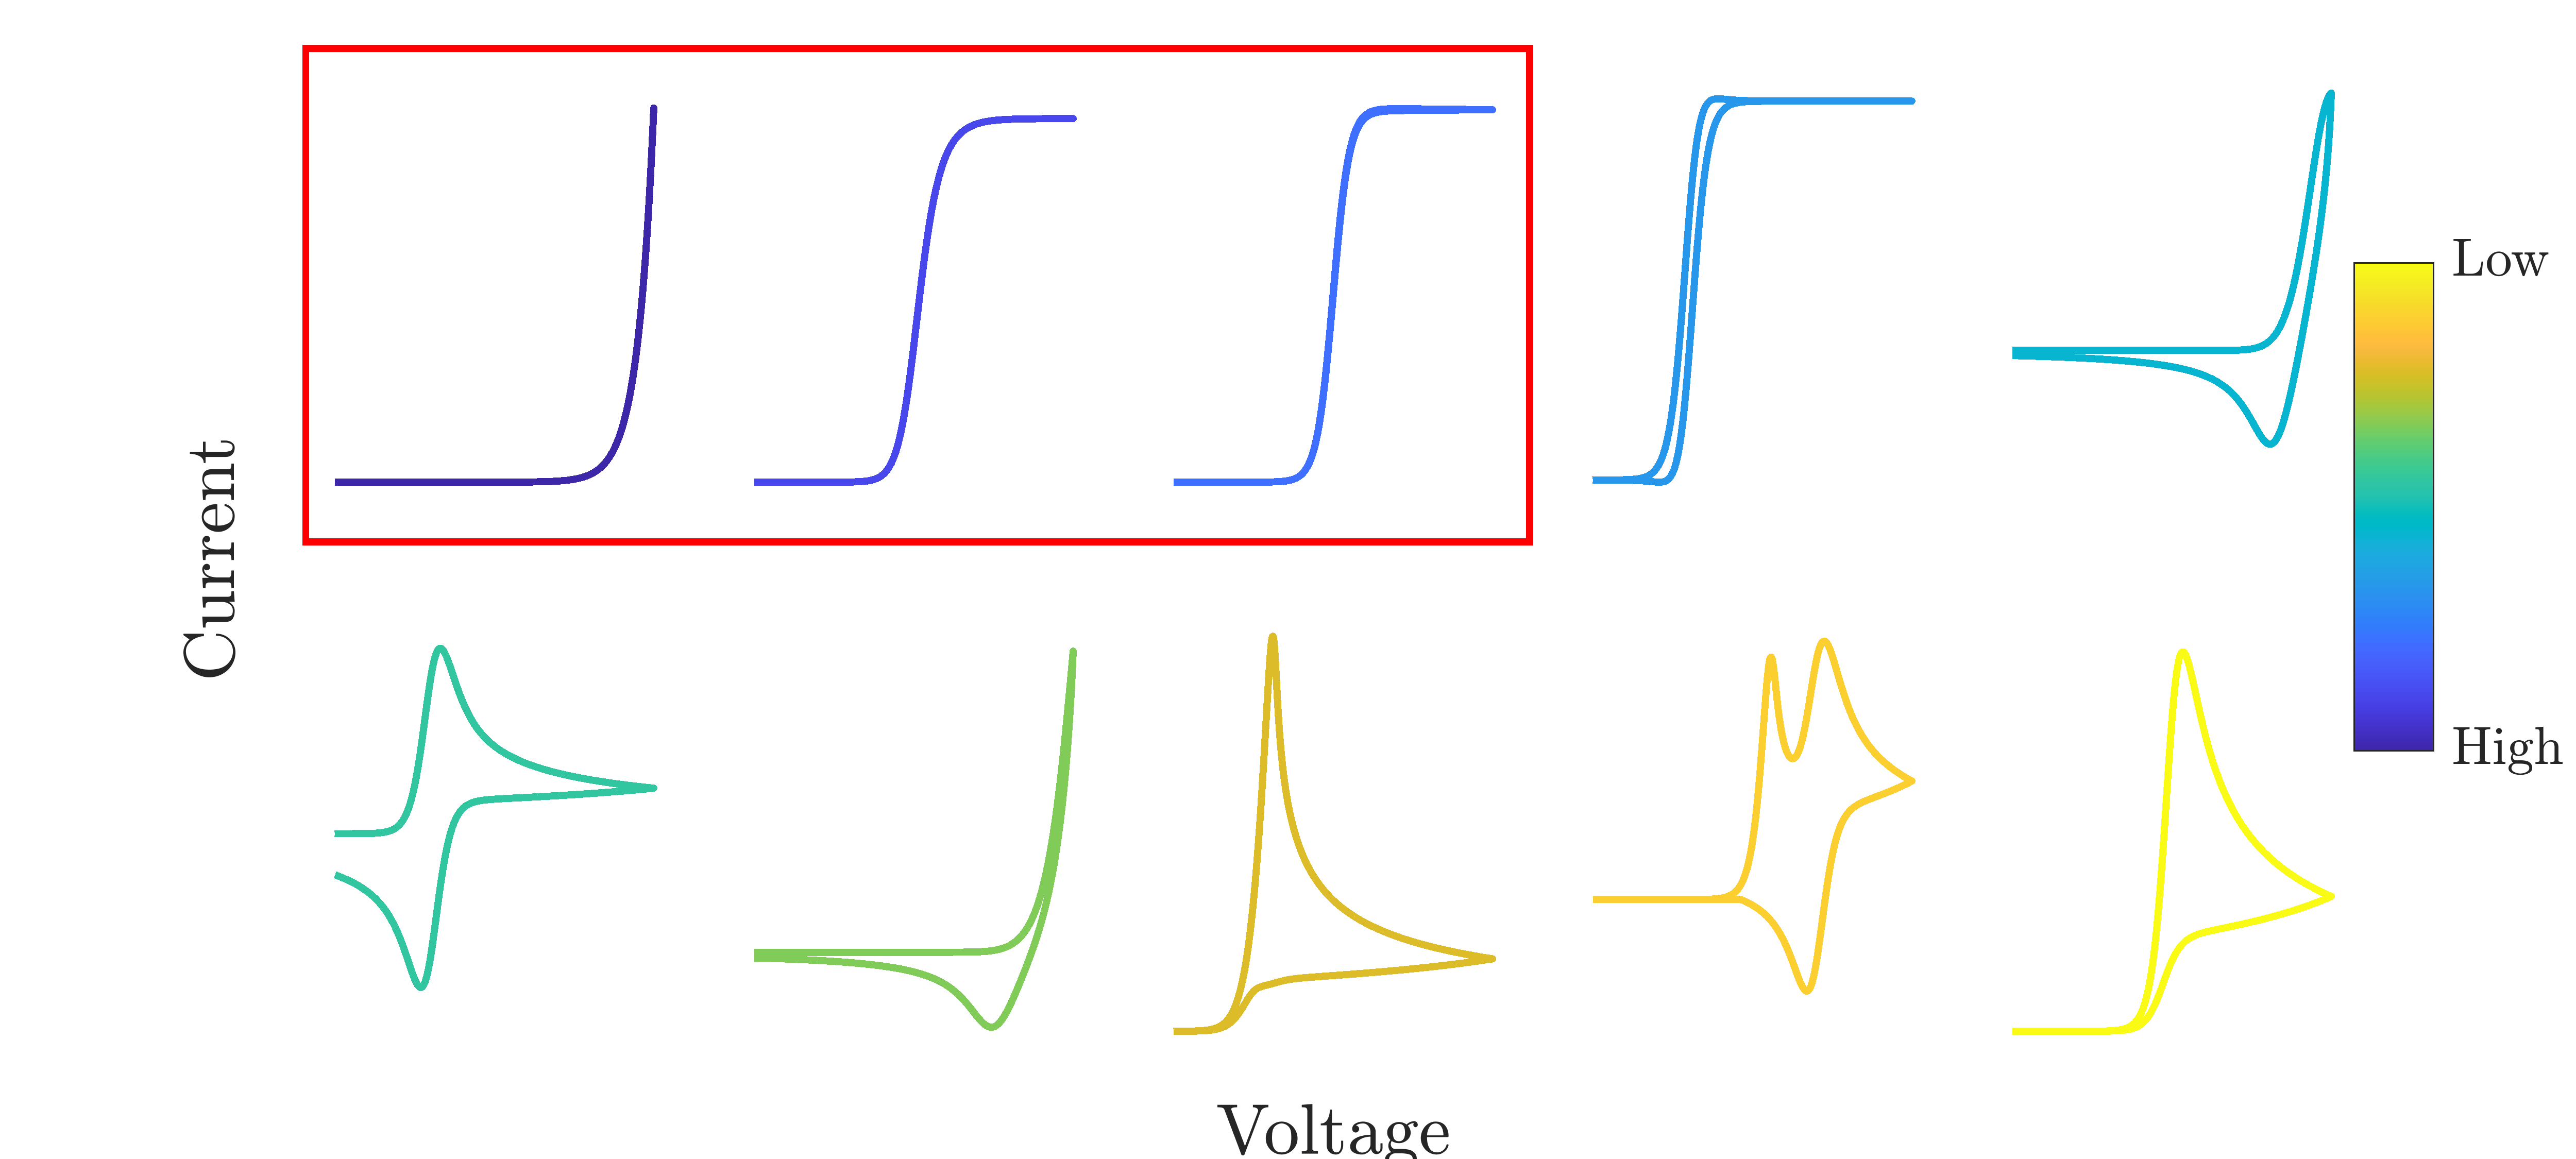
\includegraphics[width=100mm]{Chapter-3/figures/repbmsspectrum.png}
    \caption{Representative CV curves from the dataset ordered and color coded using the BMS score. CV curves boxed in red will be labelled as targets by the oracle.}
    \label{fig:repbmsscores}
\end{figure}

\subsubsection{Similarity score based oracle}
A Euclidean norm between a reference CV curve \(I_{ref}\) and any given CV curve \(I\) is computed using \(\sum \sqrt{(I - I_{ref})^2}\) both represented as vectors in a high-dimensional space and sum taken over the components. 
In~\Cref{figSI:repssscores} ten representative CV curves are depicted by sorting and color-coding based on the similarity score (similar to~\Cref{fig:repbmsscores}). 
The results showcase poor performance of the similarity score and ordering the CV curves with only two targets in the top three.
Although it marks the first curve correctly with high score, it fails to identify other S-shaped curve that is shifted along the voltage with respect to the first curve.
\begin{figure}[h]
    \centering
    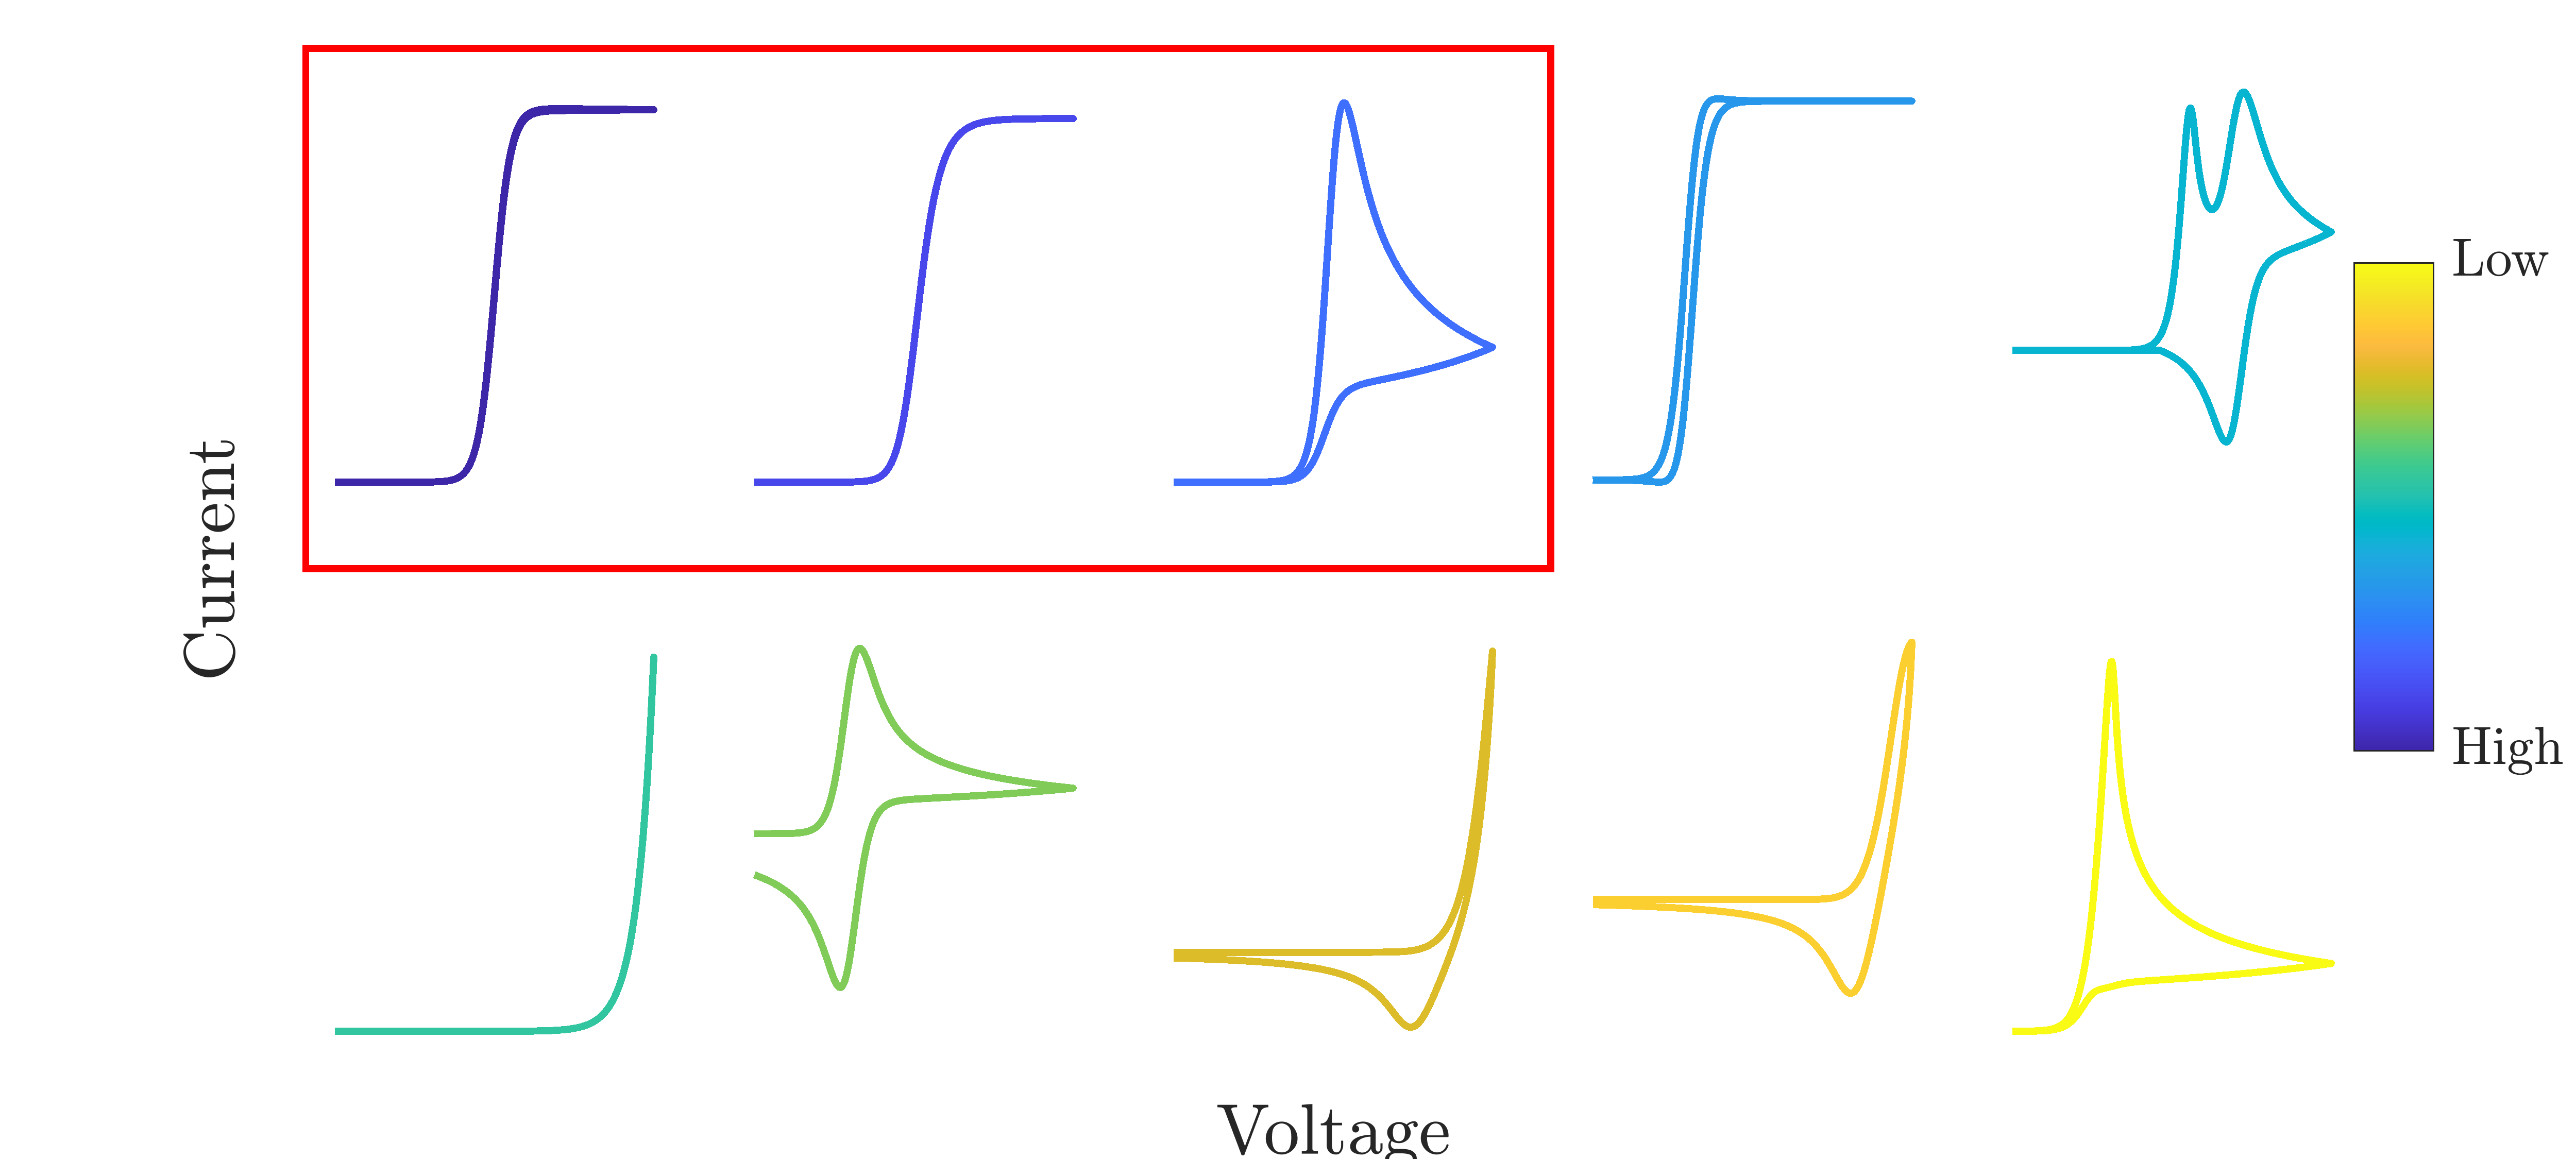
\includegraphics[width=100mm]{Chapter-3/figures/repsimscorespectrum.png}
    \caption{Representative CV curves from the dataset ordered and color coded using the similarity score. CV curves in the red box will be labelled as targets by the similarity score based oracle described here.}
    \label{figSI:repssscores}
\end{figure}

\subsubsection{FOWA-based score} 
In this subsection, a scoring method using the Foot of The Wave Analysis~(FOWA) ~\cite{costentin2015cyclic} is derived.
In the FOWA analysis, the original signal \((I,V)\) is transformed using the map \((I,V)\mapsto(I,1+\exp[\frac{F}{RT}(E-E^0)])\). 
An S-shaped CV curve is expected to be linear in two-dimensional FOWA coordinate space. 
Thus, a CV curve is scored based on its \(R^2\)-value computed with reference to user defined reference S-shape (for multiple S-shaped CV curves, maximum \(R^2\) value over the set is used), quantifying the linearity of the curve after the FOWA transformation.
~\Cref{figSI:repfowascores} is similar to~\Cref{fig:repbmsscores} with the rank of the curves determined by FOWA-based score. 
FOWA-based score ranks two of the target S-shaped CV curves in the top category. 
However, it fails to rank another S-shaped CV curve, like the fourth curve with a current onset only slightly shifted.
When discussing the effectiveness, we note that both of the approaches mentioned in this section depend on the usage of reference S-shapes from which the \(R^2\) value is computed. 
In particular, user needs to select a set of S-shapes that span the expected range in terms of current onset, rate constant etc., which is a non-trivial choice and adds to the heuristics. 
For these reasons BMS is preferred as it exploits the geometrical shape of CV curves directly without need for any user defined references. 
Moreover, note that BMS has an inherent ability to account for Gaussian noise. 
\begin{figure}[h]
    \centering
    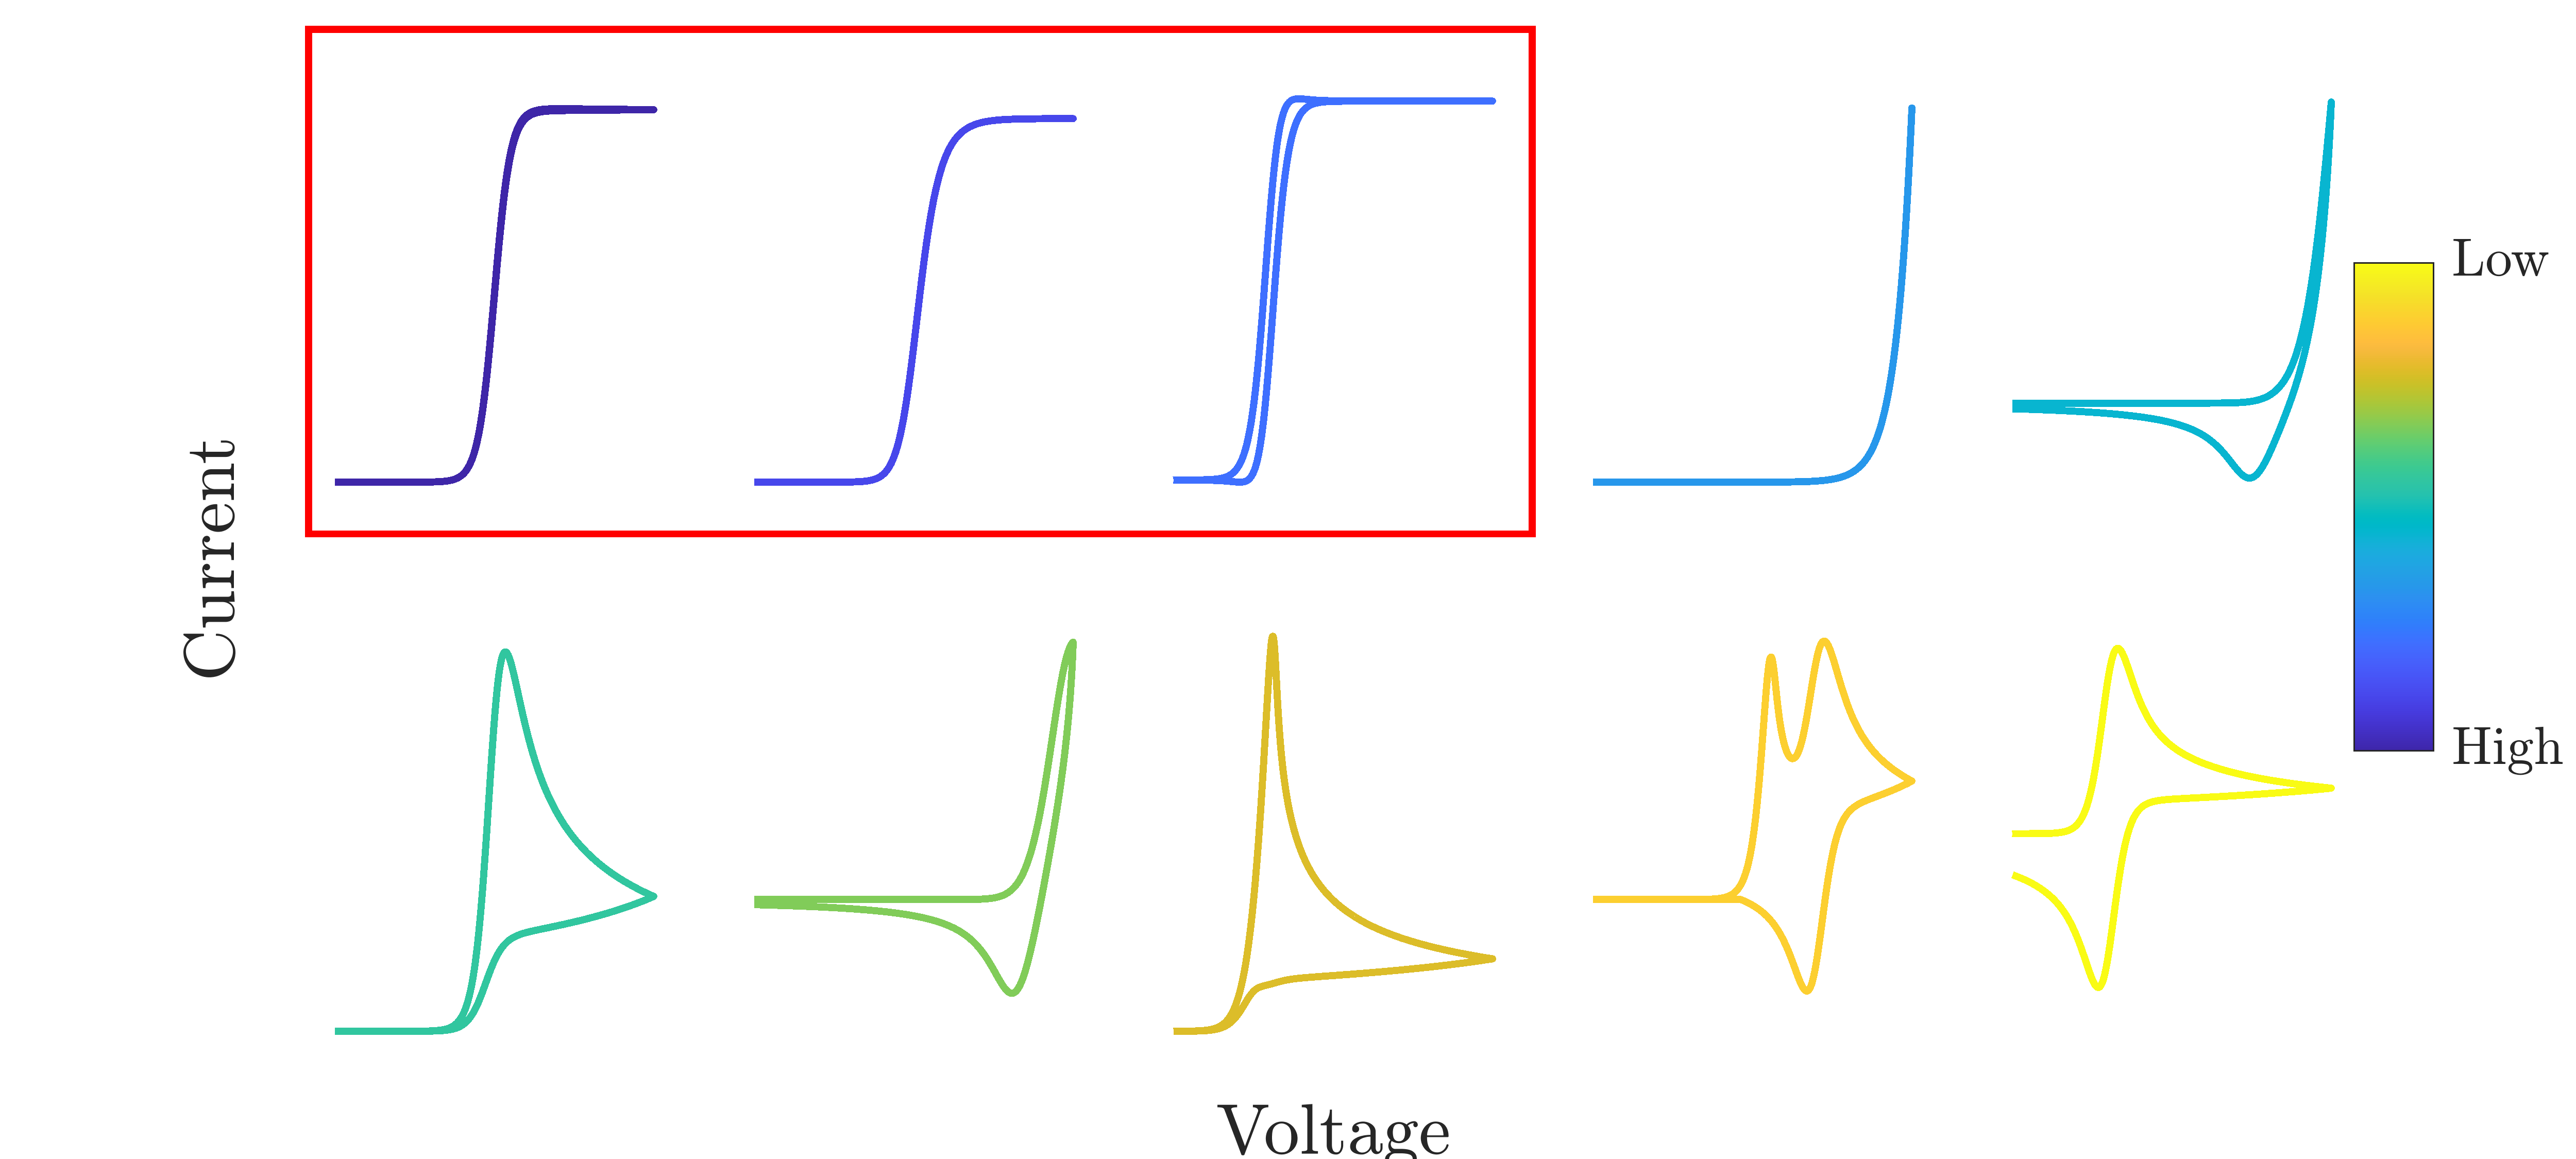
\includegraphics[width=100mm]{Chapter-3/figures/repfowaspectrum.png}
    \caption{Representative CV curves from the dataset ordered and color coded using the FOWA score. CV curves in the red box will be labelled as targets by the similarity FOWA score based oracle described here}
    \label{figSI:repfowascores}
\end{figure}

\section{Active (Batch)Search for S-shaped CV curves}
Active search with batch selection of locations in the design space has been recently studied and successfully applied to  high throughput combinatorial search of material and drug discovery~\cite{jiang2018efficient}. 
We use the state-of-the-art active batch search introduced in Jiang et.al~\cite{jiang2018efficient}, with a fixed budget of 1000 queries~(\(\approx6\%\) of exhaustive search over the grid \(\mathcal{S}\) in \Cref{tab:search_space}) to the simulator for batch sizes of \(b\in\{1,100\}\) to actively query our combinatorial search space~\(\mathcal{S}\).
The batch size reflects the setting of the high throughput analysis, as often material is prepared in batches.

A label for any given location is assigned based on the application of BMS oracle to the corresponding CV curve \(I(v,t)\) simulated by solving~\Cref{{eq:fickslaws,eq:bcs}} over \(4\times10^3\) discrete time points. 
A CV response is labelled as target if its BMS oracle score is in the range defined by top three percentile ranks~\footnote{this is a heuristic and can be altered based on application}~\footnote{Similarly for active search of bi-functional oxygen electrocatalysts, one can assign a material as a target if both of its OER and ORR experimental CV curves are in the top three percentile ranks of BMS scores. } shown in~\Cref{fig:repbmsscores}. 

\begin{figure}[h]
    \centering
    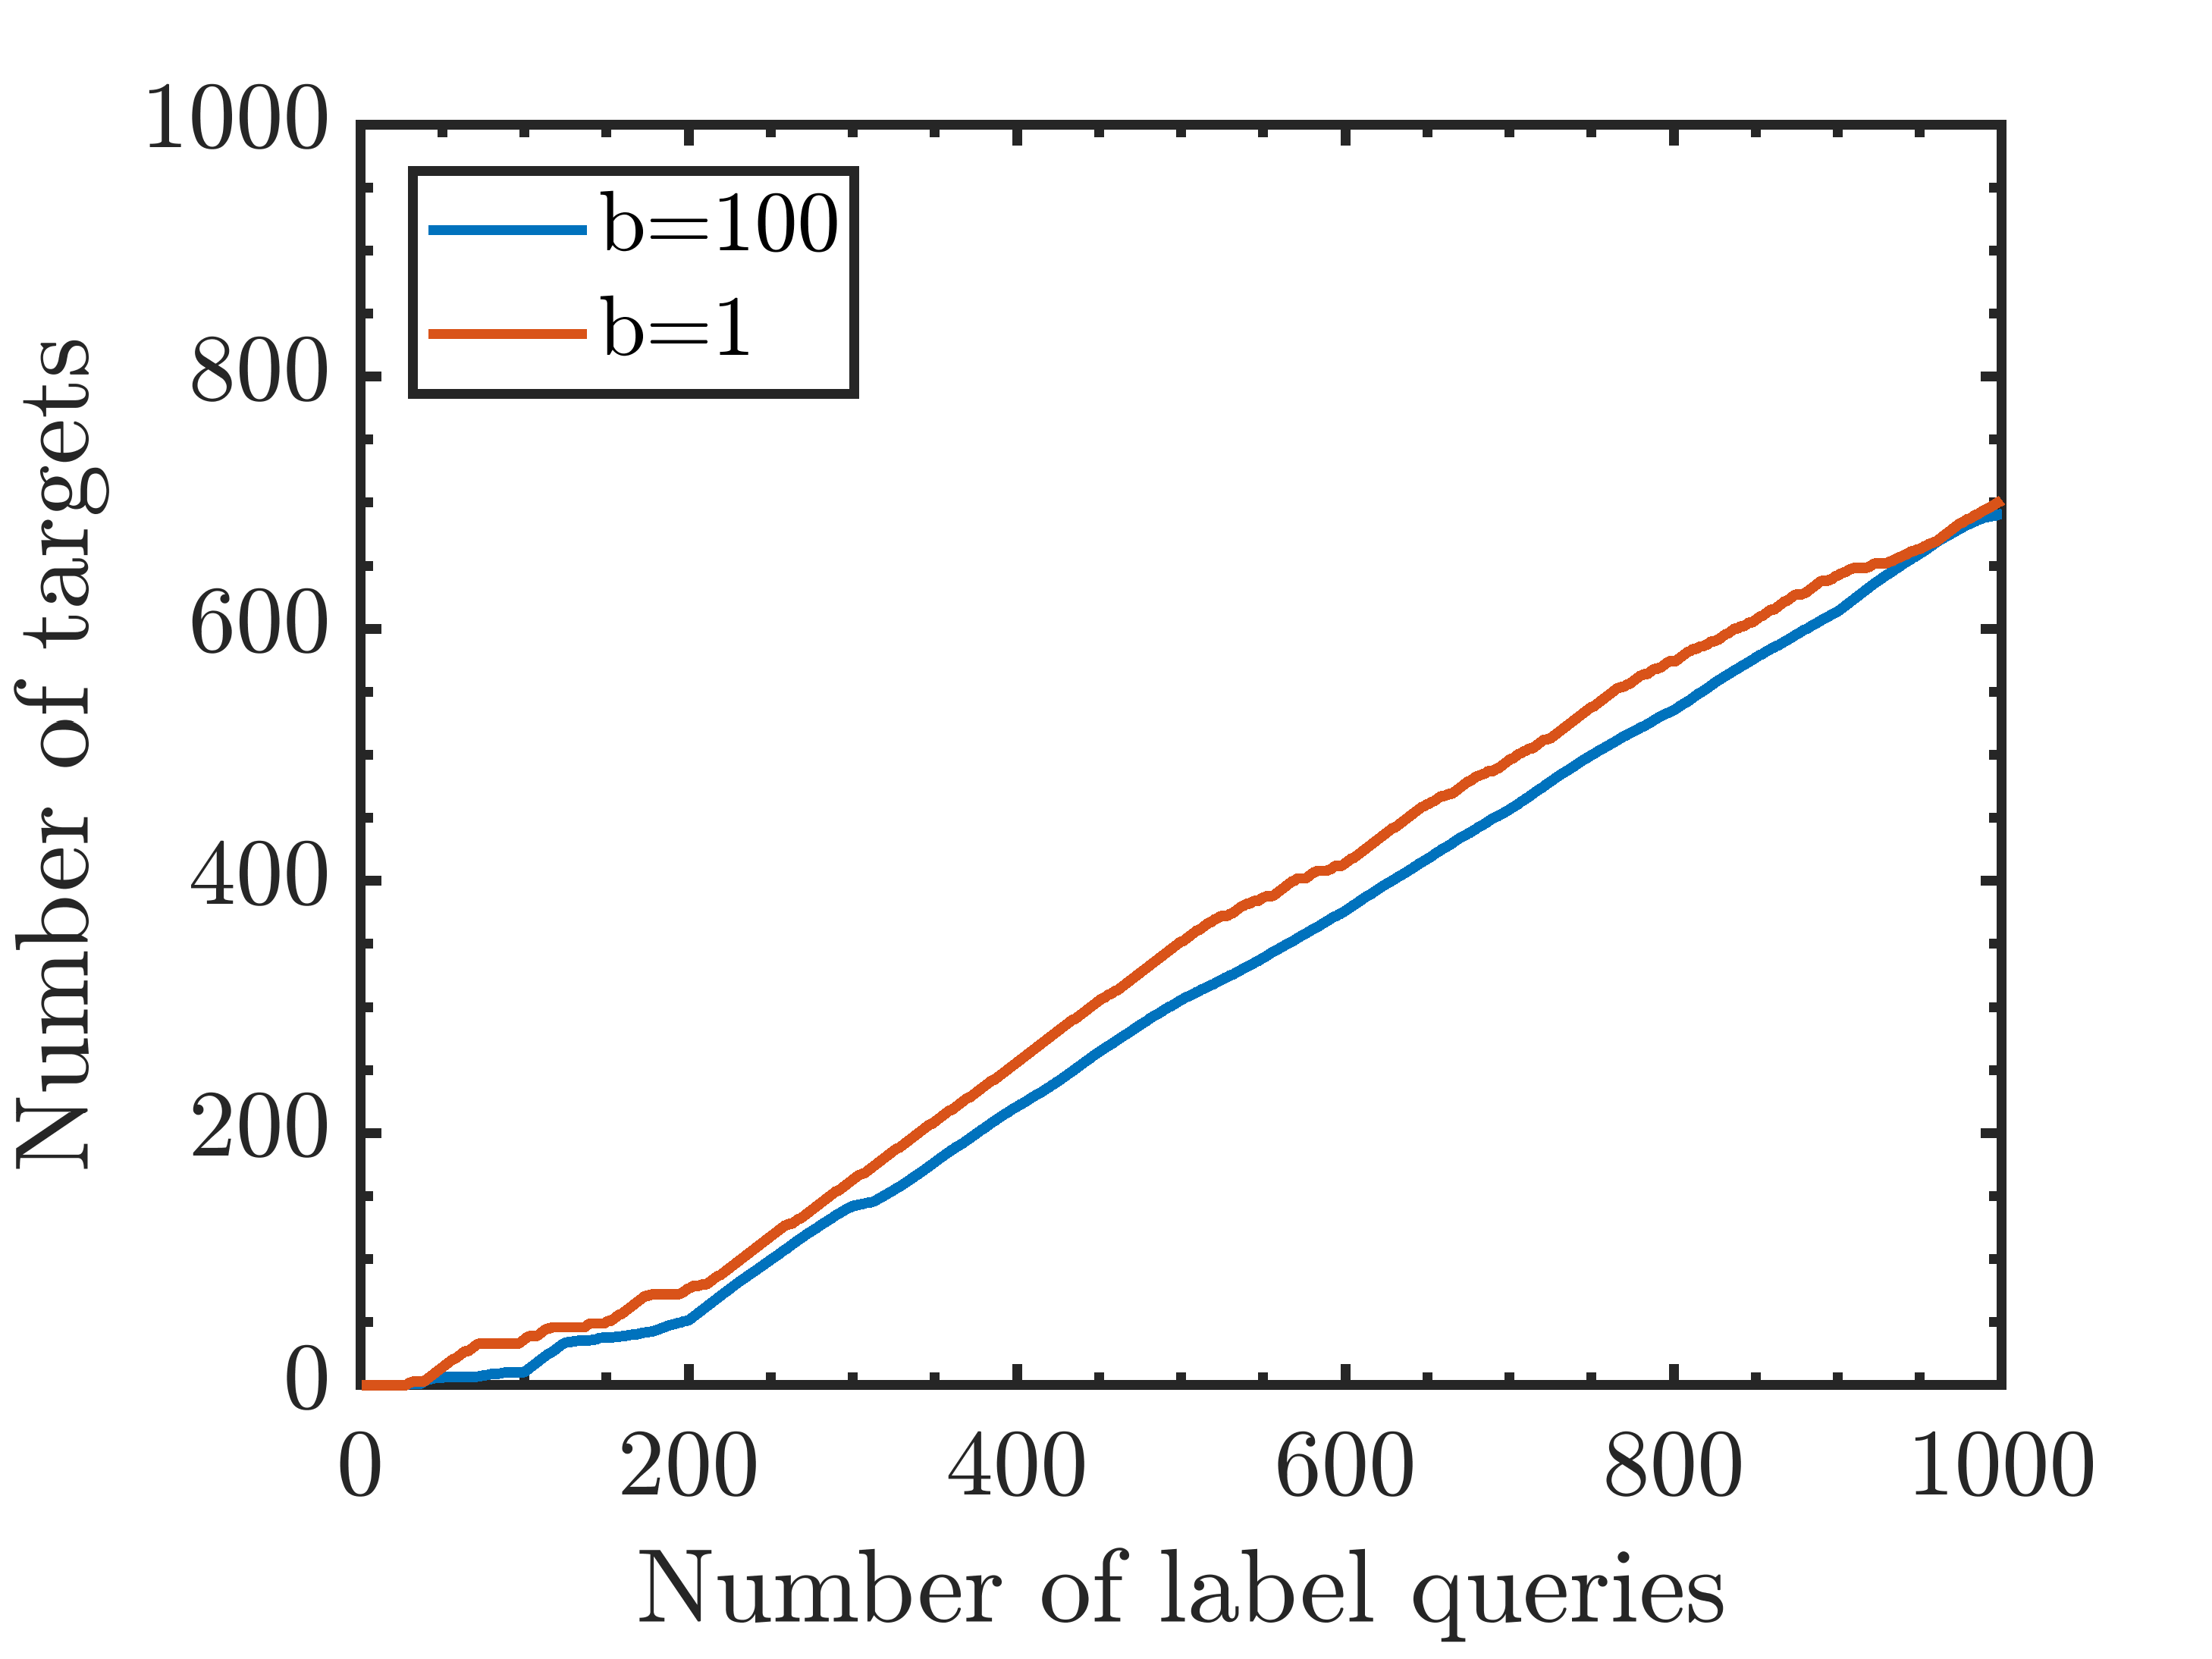
\includegraphics[width=100mm]{Chapter-3/figures/batch_results.png}
    \caption{Active target detection in the EC mechanism combinatorial search space (see~\Cref{tab:search_space} for definition of search space). We repeat the active search 20 times, each time starting with a randomly chosen non-S-shape data point in \(\mathcal{S}\). }
    \label{fig:batchens_fullec}
\end{figure}

Assuming that the design space is continuous, a \(k\)-nearest neighbor probability distribution is used a decision model in Bayesian active learning following the approach in~\cite{jiang2018efficient}. 
This assumption implies that if we find a target at a certain location in the search space, \(k\)-closest neighbors in the design space also are highly likely to be a target as well. 



In~\Cref{fig:batchens_fullec}, we report the average number of targets found in the design space over the number of label queries for two batch sizes \((b=1,100)\) considered~\footnote{The number of targets are averaged over a total of 20 active searches each time start with a randomly selected sample in the search space}.
Our results demonstrate that searching the design space using active learning can be useful, with a near linear target detection. 
It can also be noted from~\Cref{fig:batchens_fullec} for any given number of allowed label queries to the oracle~(or equivalently number of simulation queries to the simulator), the sequential selection finds marginally more targets than the batch selection \(b=100\).
This observation is in accordance with Theorem 1 in~\cite{jiang2018efficient}. 
Jiang et.al,~\cite{jiang2018efficient} argue that batch selection suffers from having to select a batch from the search space with fewer observed responses and locations. 
However, from experimental point of view, one need to consider the advantages and dis-advantages of sequential selection over batch selection. 


\section{Conclusion and future work}
In conclusion, \(\mathcal{GP}\)-based oracle is defined and evaluated for materials discovery using cyclic voltammetry.
Next, the oracle is combined with a state-of-the-art active batch search to identify conditions resulting in the targeted shape of CV curve. 
A robust high throughput combinatorial search is demonstrated to find the target responses using only \(<6\%\) of total number of CV experiments from the corresponding exhaustive search. 

As a future outlook, I anticipate that this work will have implications in identification of characterization conditions where kinetic knowledge extraction from the cyclic voltammetry can be preformed more effectively. 
Specifically, as illustrated using the active search framework, identification of S-shaped CV curves can lead to approximation rate constant of rate determining step. 
In this sense the framework discussed in this chapter has applications in accelerated knowledge extraction, with the application in screening for target catalysts including the bi-functional alkaline fuel cell catalysts that motivated this work.



\chapter{Exploratory data analysis of phase diagrams}\label{chapter4}
Organic thin films made of conjugated polymers and/or small molecules have captured the interest of the organic electronics industry due to their wide range of alterable properties (e.g., the color of light emission and solubility in organic solvents). 
High-performing devices have recently been designed with a multi-component material system (as opposed to initial studies that focused on binary blends). 
This reaffirmed the need for a holistic approach to materials design beyond binary blends used to understand the mixing behavior and morphology formation during the fabrication of multi-component organic thin films.

In this chapter, we present a thermodynamics based framework to identify the suitable solvents for a solvent-based manufacturing of organic blends. We present high throughput exploration and construction of a composition-phase diagram map that captures thermodynamics characteristics and facilitates understanding of the multi-component solution's mixing behavior. Our analysis pipeline consists of (i)~a thermodynamics based model to determine phase diagrams of multi-component mixtures using the convex hull method; and (ii)~high throughput analysis of a large set of phase diagrams using dimensionality reduction coupled with the clustering. To illustrate our pipeline, we derive the design rules for material systems typically
used in organic thin films.
\section{Introduction}
Organic thin films made of conjugated polymers and/or small molecules have captured the interest of the organic electronics industry due to their wide range of alterable properties (e.g., color of light emission and solubility in organic solvents). 
Of those properties, solubility crucially facilitates solution-based polymer processing from the liquid phase, making the materials ideal for rapid, inexpensive, large-scale, low-temperature roll-to-roll fabrication. 
Other important properties are flexibility, stretchability, softness, and compatibility with biological systems, all of which are typically absent in conventional silicon-based solutions. 
For these reasons, organic thin films have the potential to revolutionize the next generation of electronic devices within a wide array of technologies, including organic transistors, organic solar cells (OSC), and implantable medical devices and sensors.
At the current state-of-the-art, multiple processing variants exist (e.g., spin coating, doctor blading, casting, roll-to-roll manufacturing), as well as multiple variants tailored for specific materials systems (e.g., blend of polymers and small molecules).  
This proliferation of processing variants is driven by the realization that small changes in the processing can significantly improve a device's performance. 
Classic examples include changing solvents~\cite{Shaheen2001} and adding thermal annealing as a post-processing step, which have together generated organic solar cells with efficiency increased by two orders of magnitude. 
However, processing variants have been all chosen as a result of trial-and-error approaches. 
Consequently, it has remained challenging to establish reliable generalizations of material-process-morphology relationships that can be used to invert those relationships and inform new solvent-based manufacturing variant design.
In this chapter, we use the phase diagram as a representation of the thermodynamics characteristics with the goal of deriving the design rules for solvent selection in organic solar cells. 

Organic Solar Cells~(OSC), the direct application for this work, typically consists of a donor and acceptor materials sandwiched between two electrodes.
Conjugated polymer is typically selected as an electron donor, fullerene (or another polymer) is typically selected as an acceptor. 
OSC are manufactured using various methods of which we are interested in solvent based techniques where donor and acceptor polymers are mixed in a volatile solvent(s)~\cite{krebs2009fabrication}. 
During the manufacturing process, the solvent evaporates to form the morphology. 
Solvent evaporation directs the morphology evolution, and the choice of the solvent is of high importance for the final efficiency of the devices~\cite{Shaheen2001}. 
The first step towards understanding the formation of various phases in the presence of evaporating solvent (of mixture of solvents) is to study the thermodynamics of polymer mixtures. 
In this area, only recently figures of merit have been introduced to capture some characteristics of mixing behavior~\cite{ye2018miscibility}, and to establish a relationship with device properties, followed by derivation of the initial design rules~\cite{ye2018}. Also, features of phase diagrams been included in the reasoning about fabrication of OSC performance~\cite{tashvigh2015novel,li2011determination}, resulting in some initial success. 

In this chapter, we focus on the phase diagram of multi-component material system.
CALPHAD software~\cite{sundman2015opencalphad} is the most widely used tool to study phase diagrams in multi-component systems, but it focuses mostly on alloys. 
Similarly, in the area of fluid multi-component systems, similar approaches have emerged only recently~\cite{SoftMatterCEM,voskov2015ternapi}. 
In the area of organic blends, the phase diagrams of polymeric, or small molecule, multi-component material systems have been analyzed only up to ternaries~\cite{NBB07,li2011determination}. 
This is because the phase diagram construction for multi-component systems has high computational complexity. 
For example, the computational complexity of the equilibrium determination based on convex envelope method (CEM) is
\(\mathcal{O}(N_{\phi}^{(N-1)N/2})\), where \(N\) is the number of components and \(N_{\phi}\) is the number of grid points per each component~\cite{SoftMatterCEM,voskov2015ternapi}.

In this chapter, the CEM method introduced in~\cite{OryllCEM,SoftMatterCEM} is used due to its reasonable computational cost up to
quaternary systems.
We focus on material systems under fixed pressure and temperature, and aim to determine the number of phases for a given a given multi-nary composition.
CEM involves finding the equilibrium compositions of a multi-component system that can be understood by studying the Gibbs free energy landscape~\cite{GibbsCriteria1}. 
A global minimum of the Gibbs free energy landscape determines a true equilibrium state of the system while a meta-stable region is determined by local minima~\cite{OryllCEM,TangentPlaneCriteria,GibbsCriteria1}. 
CEM computes a map of composition space to its corresponding stable phases, given a free energy landscape~(comprising of composition as coordinates and energy as the height value).
The resulting map from CEM when visualized in the composition coordinates-- referred to as the \textit{phase diagram}--reveals the coexisting phases as a function of composition~\cite{SoftMatterCEM}.

We are interested in a high-throughput generation and analysis of material phase diagrams.
In particular, for solvent based OSC manufacturing, a series of experiments needs to be performed in order to select a good solvent for a given set of molecules.
This greatly limits the ability to search and evaluate large amount of solvents in a high-throughput manner.
Alternatively, one can use a phase diagram as a signature of a thermodynamic compatibility of a solvent when mixed with the set of conjugated polymers.
Techniques borrowed from machine learning allows us to study phase diagrams as points in a high-dimensional data space and analyze multiple phase diagrams together using multi-variate approaches.   
In this chapter, multi-variate approaches are used to identify subgroups in phase diagrams, obtain lower dimensional representations of the data space, that are useful in understanding statistical design rules for solvent selection. 

The rest of the chapter is arranged as follows: in \Cref{sec:cem} the convex envelope method~(CEM) to obtain a phase diagram is explained; then the CEM is applied in a high-throughput manner to generate large data sets described in \Cref{sec:htedata}; The data analysis framework is presented in \Cref{sec:pipeline} for the phase diagrams data sets and derivation of data-driven design rules for solvent selection in organic blend manufacturing are demonstrated in \Cref{sec:results}.    

\section{Methods}
\subsection{Phase diagram generation}\label{sec:cem}
Gibbs phase stability states that a globally stable equilibrium state can be obtained by constructing (lower) convex hull of energy over composition~\cite{OryllCEM,SoftMatterCEM}. 
A phase diagram can be determined by applying Gibbs stability criteria of energy landscape~\cite{GibbsCriteria1} using the convex envelope method~(CEM) introduced in~\cite{OryllCEM,SoftMatterCEM}.
According to Gibbs rules, stable compositions lie on the convex hull of energy landscape while unstable compositions lie above.
The CEM is generic and can be applied to any given energy function form. 
Two forms of energy functions are evaluated: polynomial and Flory-Huggins.
The later is used to study the multi-component organic blend system and is defined using the generalized form for an \(N\) component system given by~\Cref{eq:FH}. 
\begin{equation}\label{eq:FH}
    f_{\text{FH}} = \sum_{i=1}^{N}  \frac{1}{M_i} \phi_{i}\lnn{\phi_i} + \sum_{i=1}^{N}\sum_{j(\neq i)=1}^{N}\phi_i \phi_j \chi_{ij}
\end{equation}
where \(\phi\) is composition defined in terms of volume fraction , \(N\) is total number of components in the mixture, \(\chi_{ij}\) are Flory-Huggins interaction parameters between components \(i,j\) and \(M_i\) is degree of polymerization of \(i^{th}\) compound. 

A step-by-step procedure of CEM is described below and an example is shown in~\Cref{fig:workflow} for a three component system (i.e. \(N=3\)).
\begin{enumerate}\label{algo:cem}
    \item[Input:] Free energy function, desired mesh size
    \item[1.] \textbf{Grid generation:} Create a grid \(G\) using an user-defined mesh size $N_{\phi}$ (in terms of number of points per component/dimension) as an n-dimensional hyperplane of compositions (volume fractions \(\{\phi_i\}_{i=1}^{n}\)).
    \item[2.] \textbf{Compute free energy landscape:} Evaluate free energy at each point in \(G\). This results in a (discrete) energy landscape. 
    \item[3.] \textbf{Compute convex envelope:} Compute the convex hull of energy landscape. 
    \item[4.] \textbf{Lower convex hull}: Obtain a lower convex hull~\footnote{Given a energy landscape as a set of points and a height function (energy) , one can obtain the lower convex hull by first adding a point at infinity height to the set and then excluding the simplices that connect to it.} and project it to \(G\) by simply looking up the vertex indices resulting in a mesh of \(G\). 
    The outcome from this step is the projected lower hull, \(G_l\), where vertices corresponds to the points in \(G\).
    \item[5.] \textbf{Compute phase labels:} For each simplex in the mesh $G_l$, assign a phase label based on the number of connected components (as described in~\cite{SoftMatterCEM}). 
    An user defined threshold \(\Delta\) is used to compute adjacency matrix which in turn is used to compute number of connected components.
    \item[Output:] Phase diagram represented as $G_l$ with the phase label assigned to each simplex. 
\end{enumerate}

\begin{figure}[h]
    \centering
    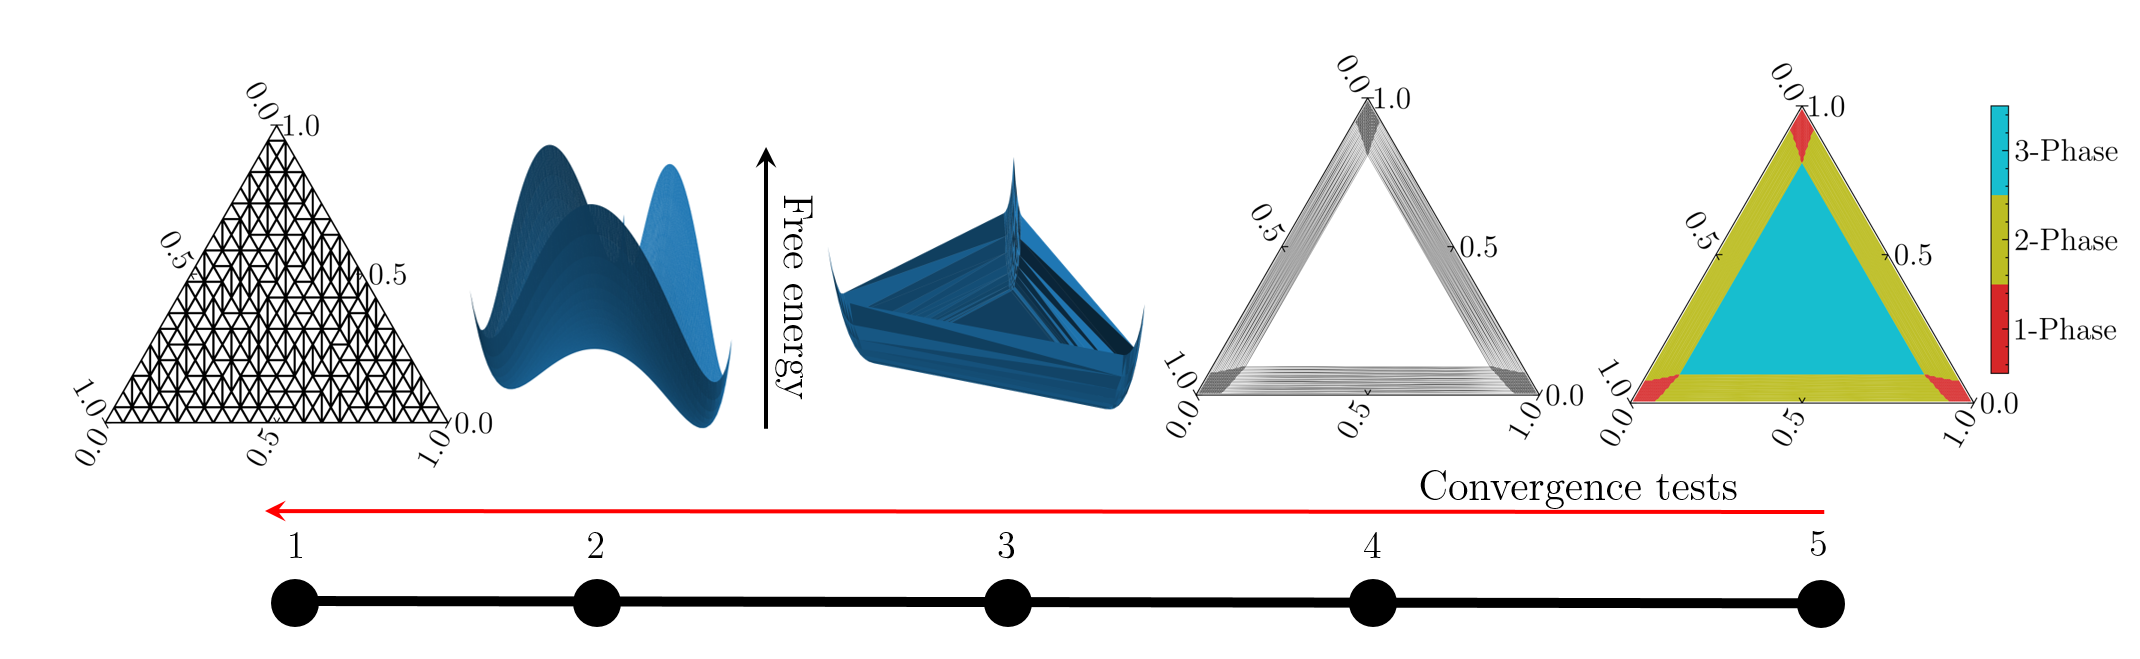
\includegraphics[width=\textwidth]{Chapter-4/figures/CEM_workflow.png}
    \caption{Convex envelope method visualized as a step-by-step process (1-5) with the series of tests performed. The red arrows depict where the tests can be performed and iterated until convergence, if required.}
    \label{fig:workflow}
\end{figure}

Two representations of phase diagrams are used:
The first representation corresponds to the output from~\Cref{algo:cem} and is referred as simplex-indexed set representation. 
The second representation is a a set indexed on the initial uniform grid $G$ (step 1 of~\Cref{algo:cem}), and is referred as a grid-indexed set representation.
The advantage of the second representation is the fixed size that ease the distance calculation. 
The grid-indexed representation is obtained from the simplex-indexed representation by assigning the phase label for each point in the grid by mapping it to the corresponding simplex in the convex envelope. 
The grid-indexed representation is used for the data analysis in~\Cref{sec:pipeline} and differentiate it from its simplex-indexed representation by a change of color-code while visualizing the phase diagram.

\section{Data generation}~\label{sec:htedata}
In ~\Cref{sec:pipeline}, a data-analysis pipeline is described to be applied on a relatively large sets of phase diagrams data described in~\Cref{sec:htedata}.
To derive the design rules we first perform dimensionality reduction followed by clustering. A overview of the dimensionality reduction and clustering methods can be found in~\ref{appendixB}.

The design space of variables are interaction parameter \(\chi\) values in~\Cref{eq:FH}.
The test case involves uniformly sampling the \(\chi\) values to be used in~\Cref{eq:FH} for a three component system. 
A uniform three-dimensional design space is defined via \(\chi_{12}\in[1.3,1.335,1.37,1.405,1.44]\) and 
\(\chi_{13}, \chi_{23}\in[0.3,0.6,1,1.5,2,2.5,3]\) a total of 245 phase diagrams are generated using the CEM method described in~\Cref{algo:cem}. 
The degree of polymerization for three materials are kept constant: $M_1=10$ for polymer, $M_2=10$ for small molecule, $M_3=1$ for solvent.
The goal using the model data set is to study the following question: \textit{given a densely sampled design space of phase diagram, can we automatically group various types of phase diagrams in the data set using clustering?}

\section{Data analysis pipeline}\label{sec:pipeline}
The data analysis pipeline as depicted in~\Cref{fig:mlpipeline} is as follows:~a) Generate a set of phase diagrams using the CEM in a high-throughput manner;~b) Compute pairwise similarities are and store in a matrix \(M\);~c) Apply clustering and dimensionality reduction to \(M\).
Spectral clustering method is used to obtain subgroups that are highly correlated within but not across using a Gaussian similarity of \(M\)~\cite{SpectralClustering}. 
A multi-dimensional scaling~(MDS)~\cite{ESL} of \(M\) is used to obtain a lower-dimensional representation using eigenvalues of \(M\) where each phase diagram can be represented using a point in a Cartesian coordinate system.
MDS and spectral clustering are performed using the \textit{scikit-learn}~\cite{sklearn} and other dependent python packages: scipy~\cite{scipy}, matplotlib~\cite{matplotlib} and mpltern~\cite{mpltern}.
Analyzing the lower dimensional representations and clustered subgroups together, allows users to decipher potential design rules that connect any two subgroups of phase diagrams. In \Cref{appendixB}, a detailed description of dimensionality reduction and clustering is provided with emphasis on geometrical interpretation of the methods used in this thesis.

The key element of the pipeline is the choice of the distance or similarity measure. The most commonly used distance is Euclidean norm, but other distances have been used~\cite{FiftySix}. 
In this work, we chose a \textit{Hamming} distance~(\Cref{eq:hamming}) between two grid-indexed representation of phase diagrams.

The point indexed phase diagram vectors are visualized by color-coding each point (instead of each simplex as before) in red (1-phase), green (2-phase) and blue (3-phase) as shown in (a) of~\Cref{fig:mlpipeline}.
The distance is then computed between a pair of phase label sets \(u,v\) indexed by composition using~\Cref{eq:hamming}.
\begin{equation}\label{eq:hamming}
    d(u,v) = \frac{1}{\ell}\sum_{i}\delta_{u[i],v[i]}
\end{equation}
where \(\delta_{ij}\) is the Kronecker-delta function and \(\ell\) is the cardinality of sets \(u,v\).
The Hamming distance is agnostic to the dimensionality of the grid \(G\), easy to compute thus making it a good choice for phase diagrams.  

\begin{figure}[h]
    \centering
    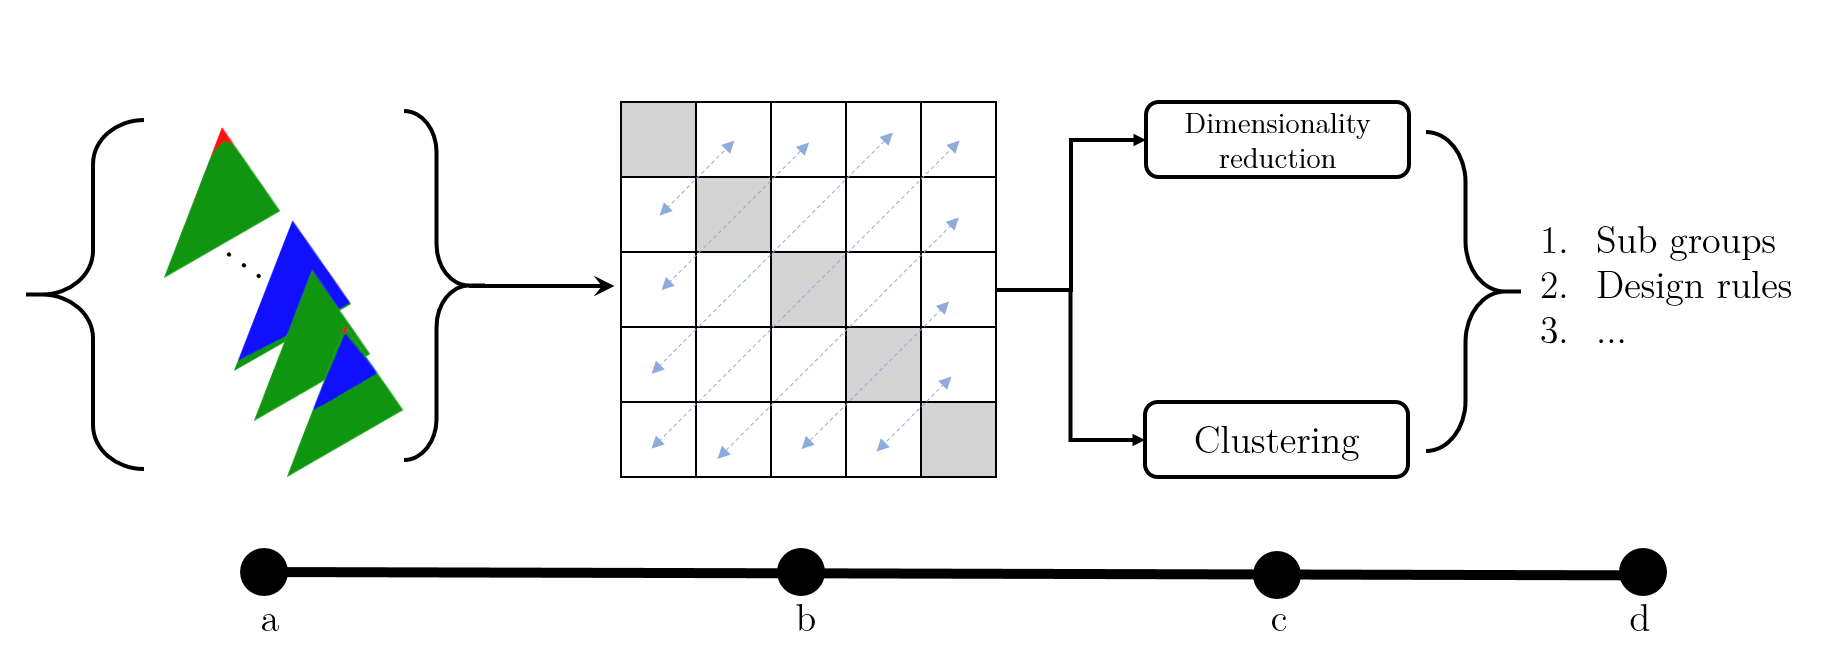
\includegraphics[width=\textwidth]{Chapter-4/figures/analysis_pipepline.png}
    \caption{Data analysis pipeline}
    \label{fig:mlpipeline}
\end{figure}


\section{Results and Discussions}\label{sec:results}
\subsection{Clustering phase diagrams}\label{sec:res:ct1}
\Cref{fig:result2_synthetic_mds} depicts a two-dimensional representation obtained using MDS with each point corresponding to a phase diagram in the model data set. 
The points are color-coded based on their spectral clustering labels (with a total of five clusters).
In \Cref{fig:result2_synthetic_clusters} we show the representative phase diagrams for each cluster. 
We observe that clusters in~\Cref{fig:synthdata} have distinct features: phase diagrams without any three phase regions (cluster 0); dominant in three phase region (cluster 1); all compositions belonging to three phase (cluster 2); mix of two and three phase regions (cluster 3,4) that differ in the direction of the phase boundary.
It is difficult to determine a way to obtain true clusters: We do more of a context-driven clustering where the hamming distance and number of clusters justify the true/real clusters (See section 5.3 in \cite{TrueClusters}).
In~\Cref{fig:synth_designspace}, we depict the \(\chi\) space sampling as points with \(\chi_{12},\chi_{13}, \chi_{23}\) as coordinate axes. 
The points are then colored based on the clustering label shown in \Cref{fig:result2_synthetic_mds}.
One can observe that the clusters show a radially evolving arrangement, which can be clearly seen in the two-dimensional projection of the design space shown in~\Cref{fig:synth_designspace_2D}.

\begin{figure}[h]\label{fig:synthdata}
    \centering
    \begin{subfigure}[b]{0.48\textwidth}
        \centering
        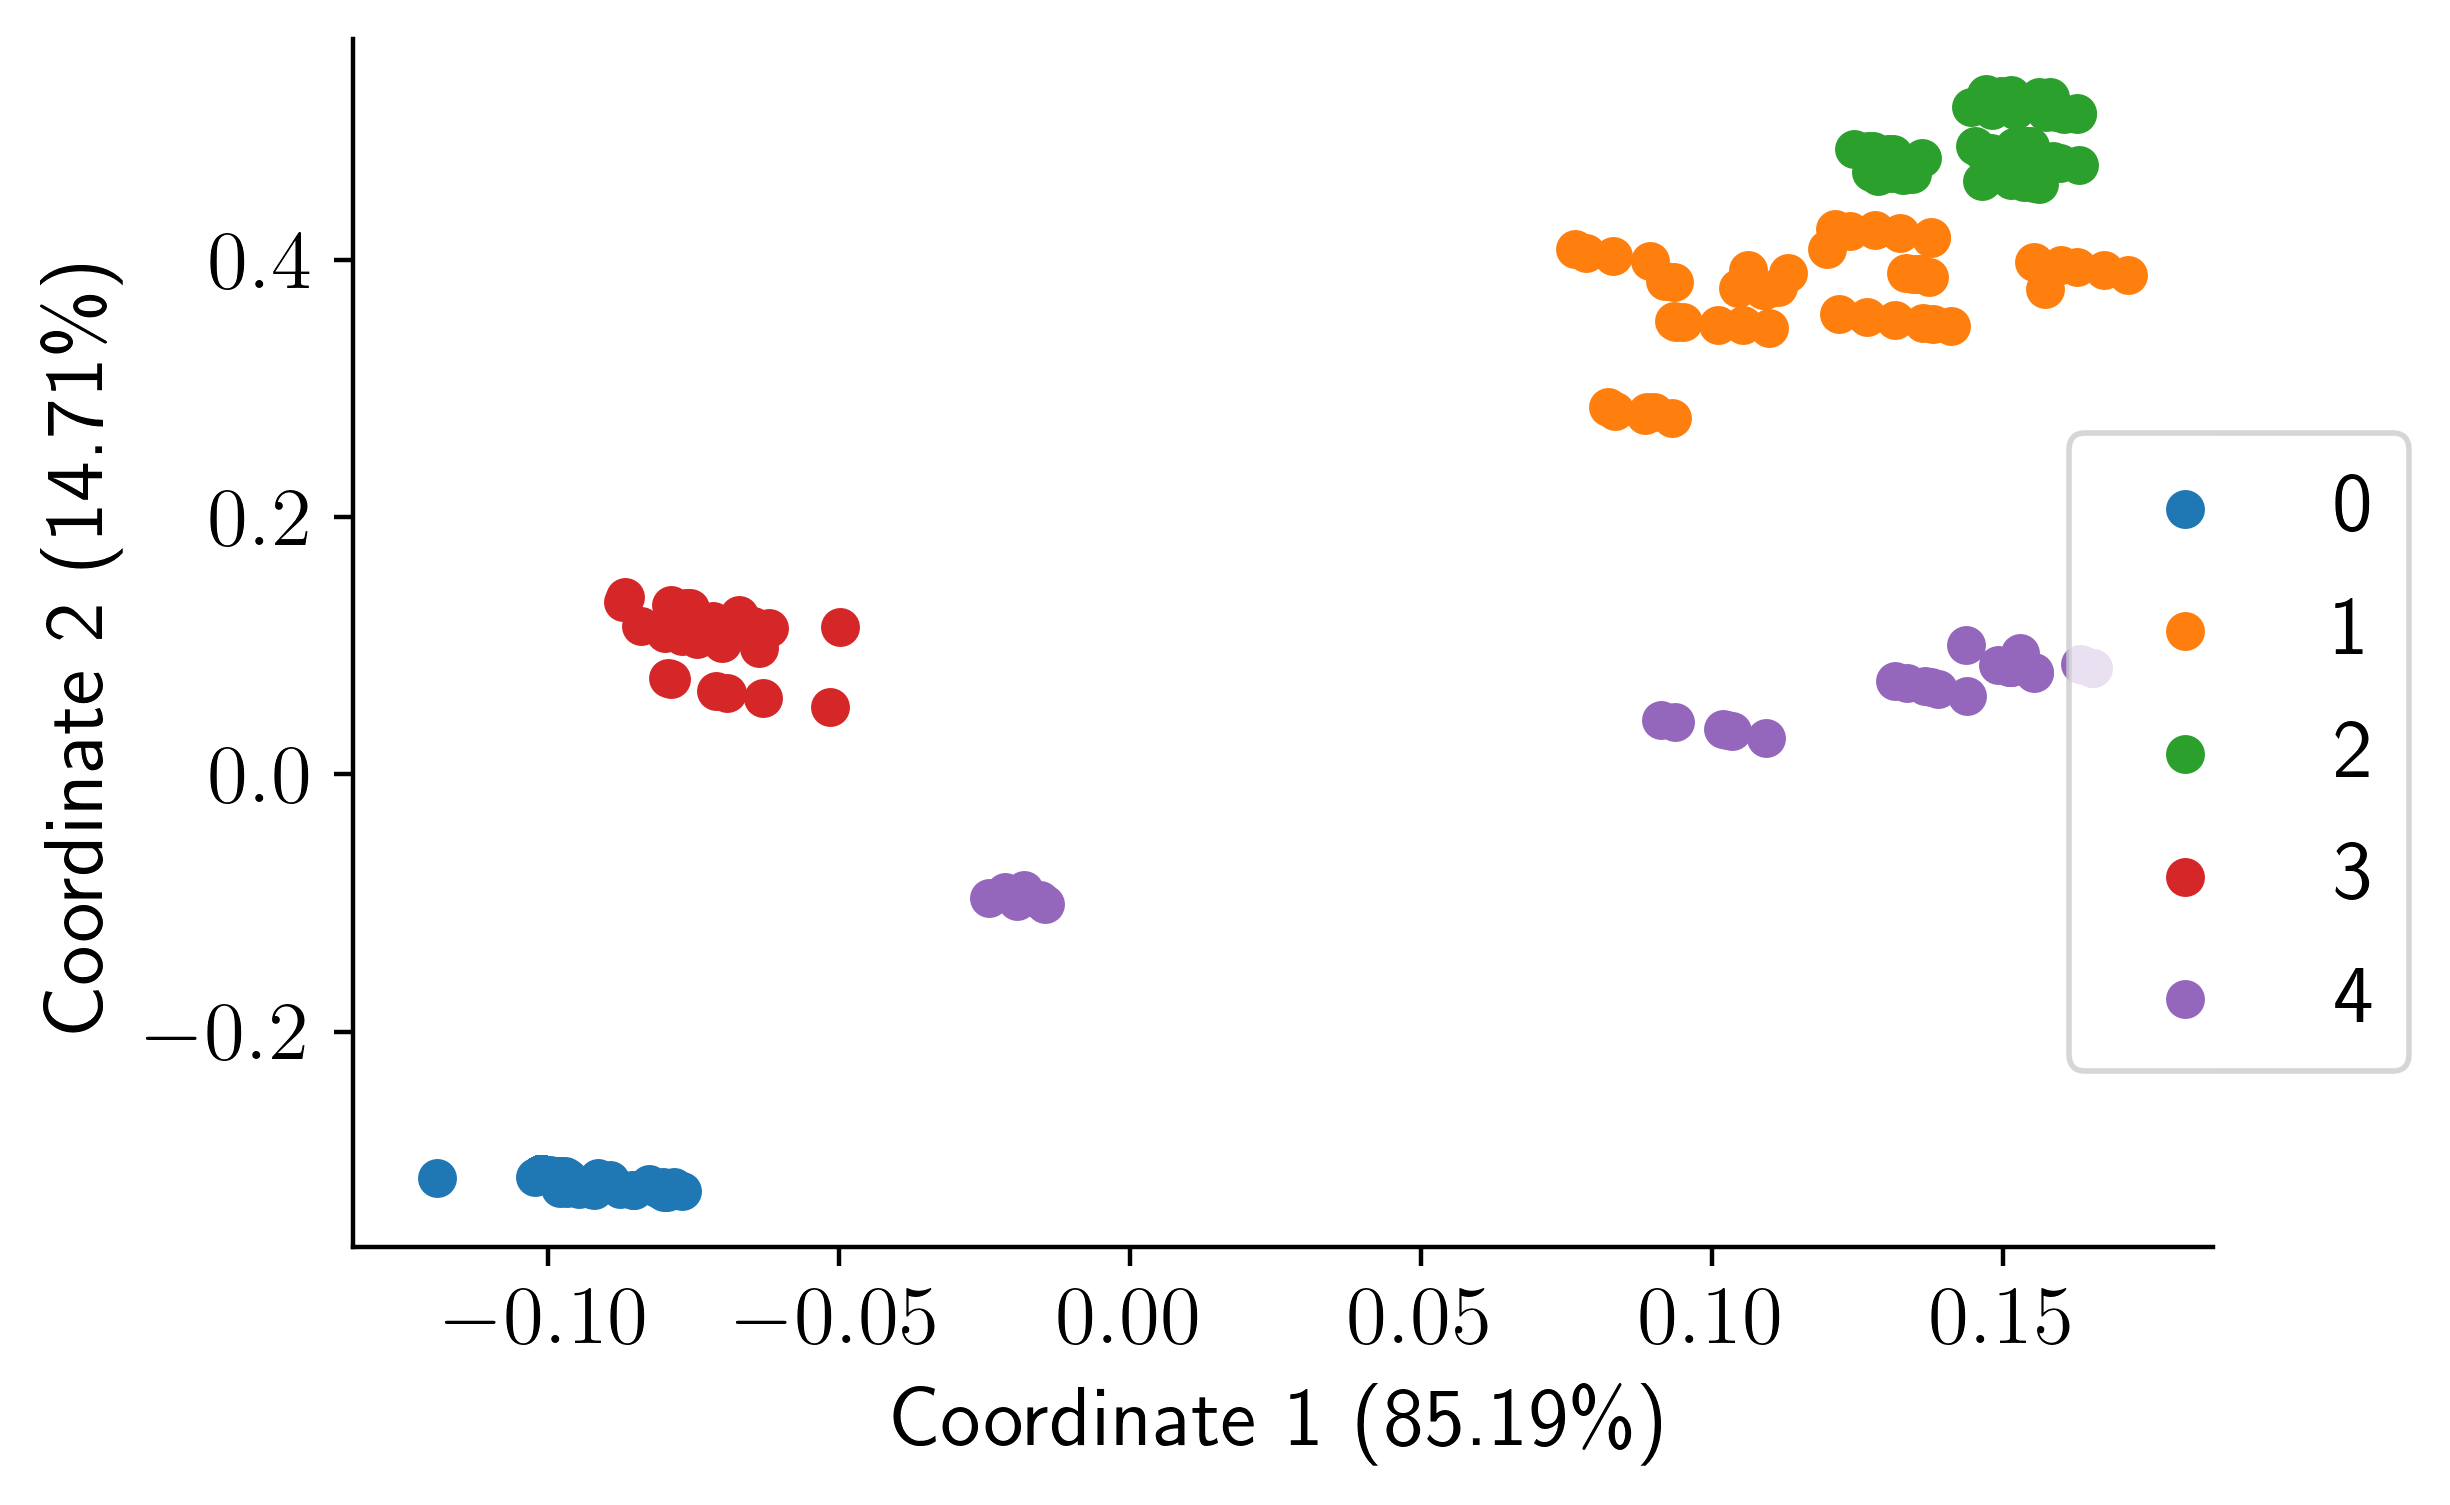
\includegraphics[width=\textwidth]{Chapter-4/figures/result2/result2_Synthetic_MDS.png}
        \label{fig:result2_synthetic_mds}
    \end{subfigure}
    \hfill
    \begin{subfigure}[b]{0.48\textwidth}
        \centering
        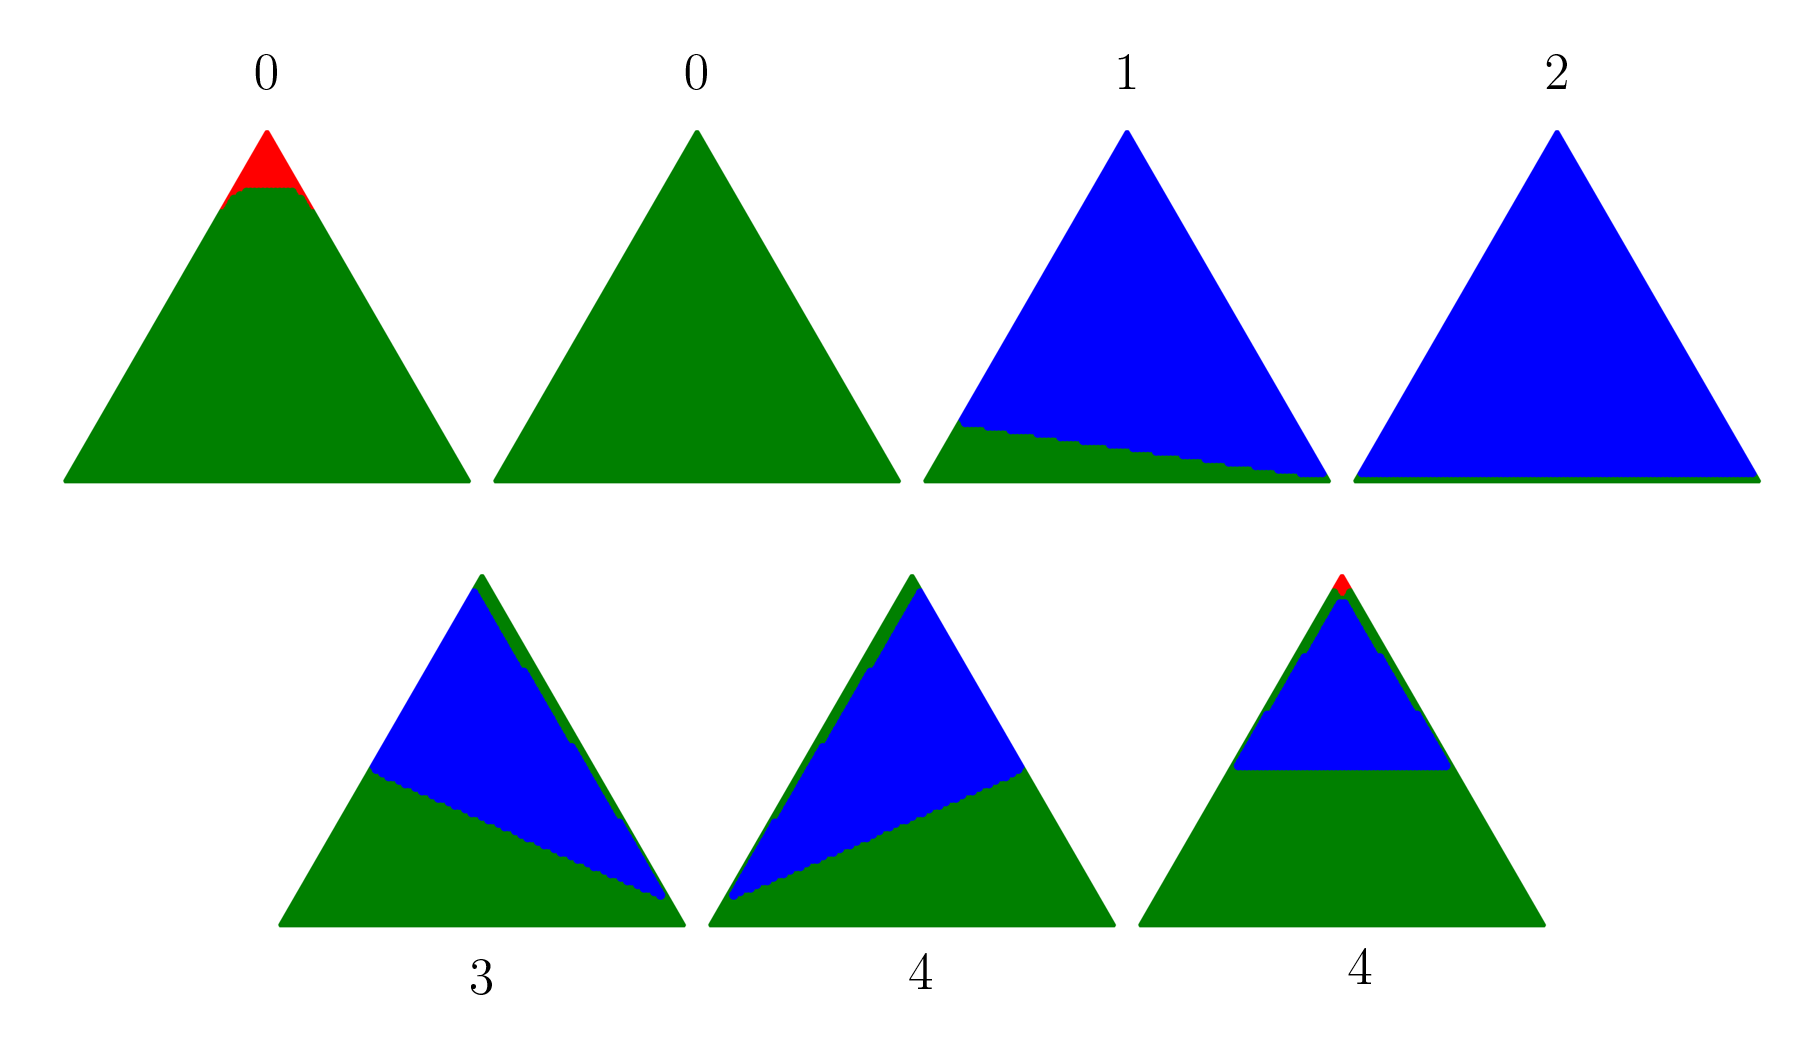
\includegraphics[width=\textwidth]{Chapter-4/figures/result2/result2_synthetic_clusters_manual.png}
        \caption{}
        \label{fig:result2_synthetic_clusters}
     \end{subfigure}
    \caption{Application of data analysis pipeline in \Cref{fig:mlpipeline} to mode data set in \Cref{sec:htedata}. (a) The lower dimensional Euclidean representation of the distance metric \(M\) for the space of 245 phase diagrams obtained for dataset presented in~\Cref{sec:htedata} using MDS. The color-code corresponds to the spectral clustering label. (b) Representative phase diagrams of clusters obtained from spectral clustering of metric \(M\). See text above for the discussion.}
\end{figure}

\begin{figure}[h]
    \centering  
    \begin{subfigure}[b]{0.4\textwidth}
        \centering
        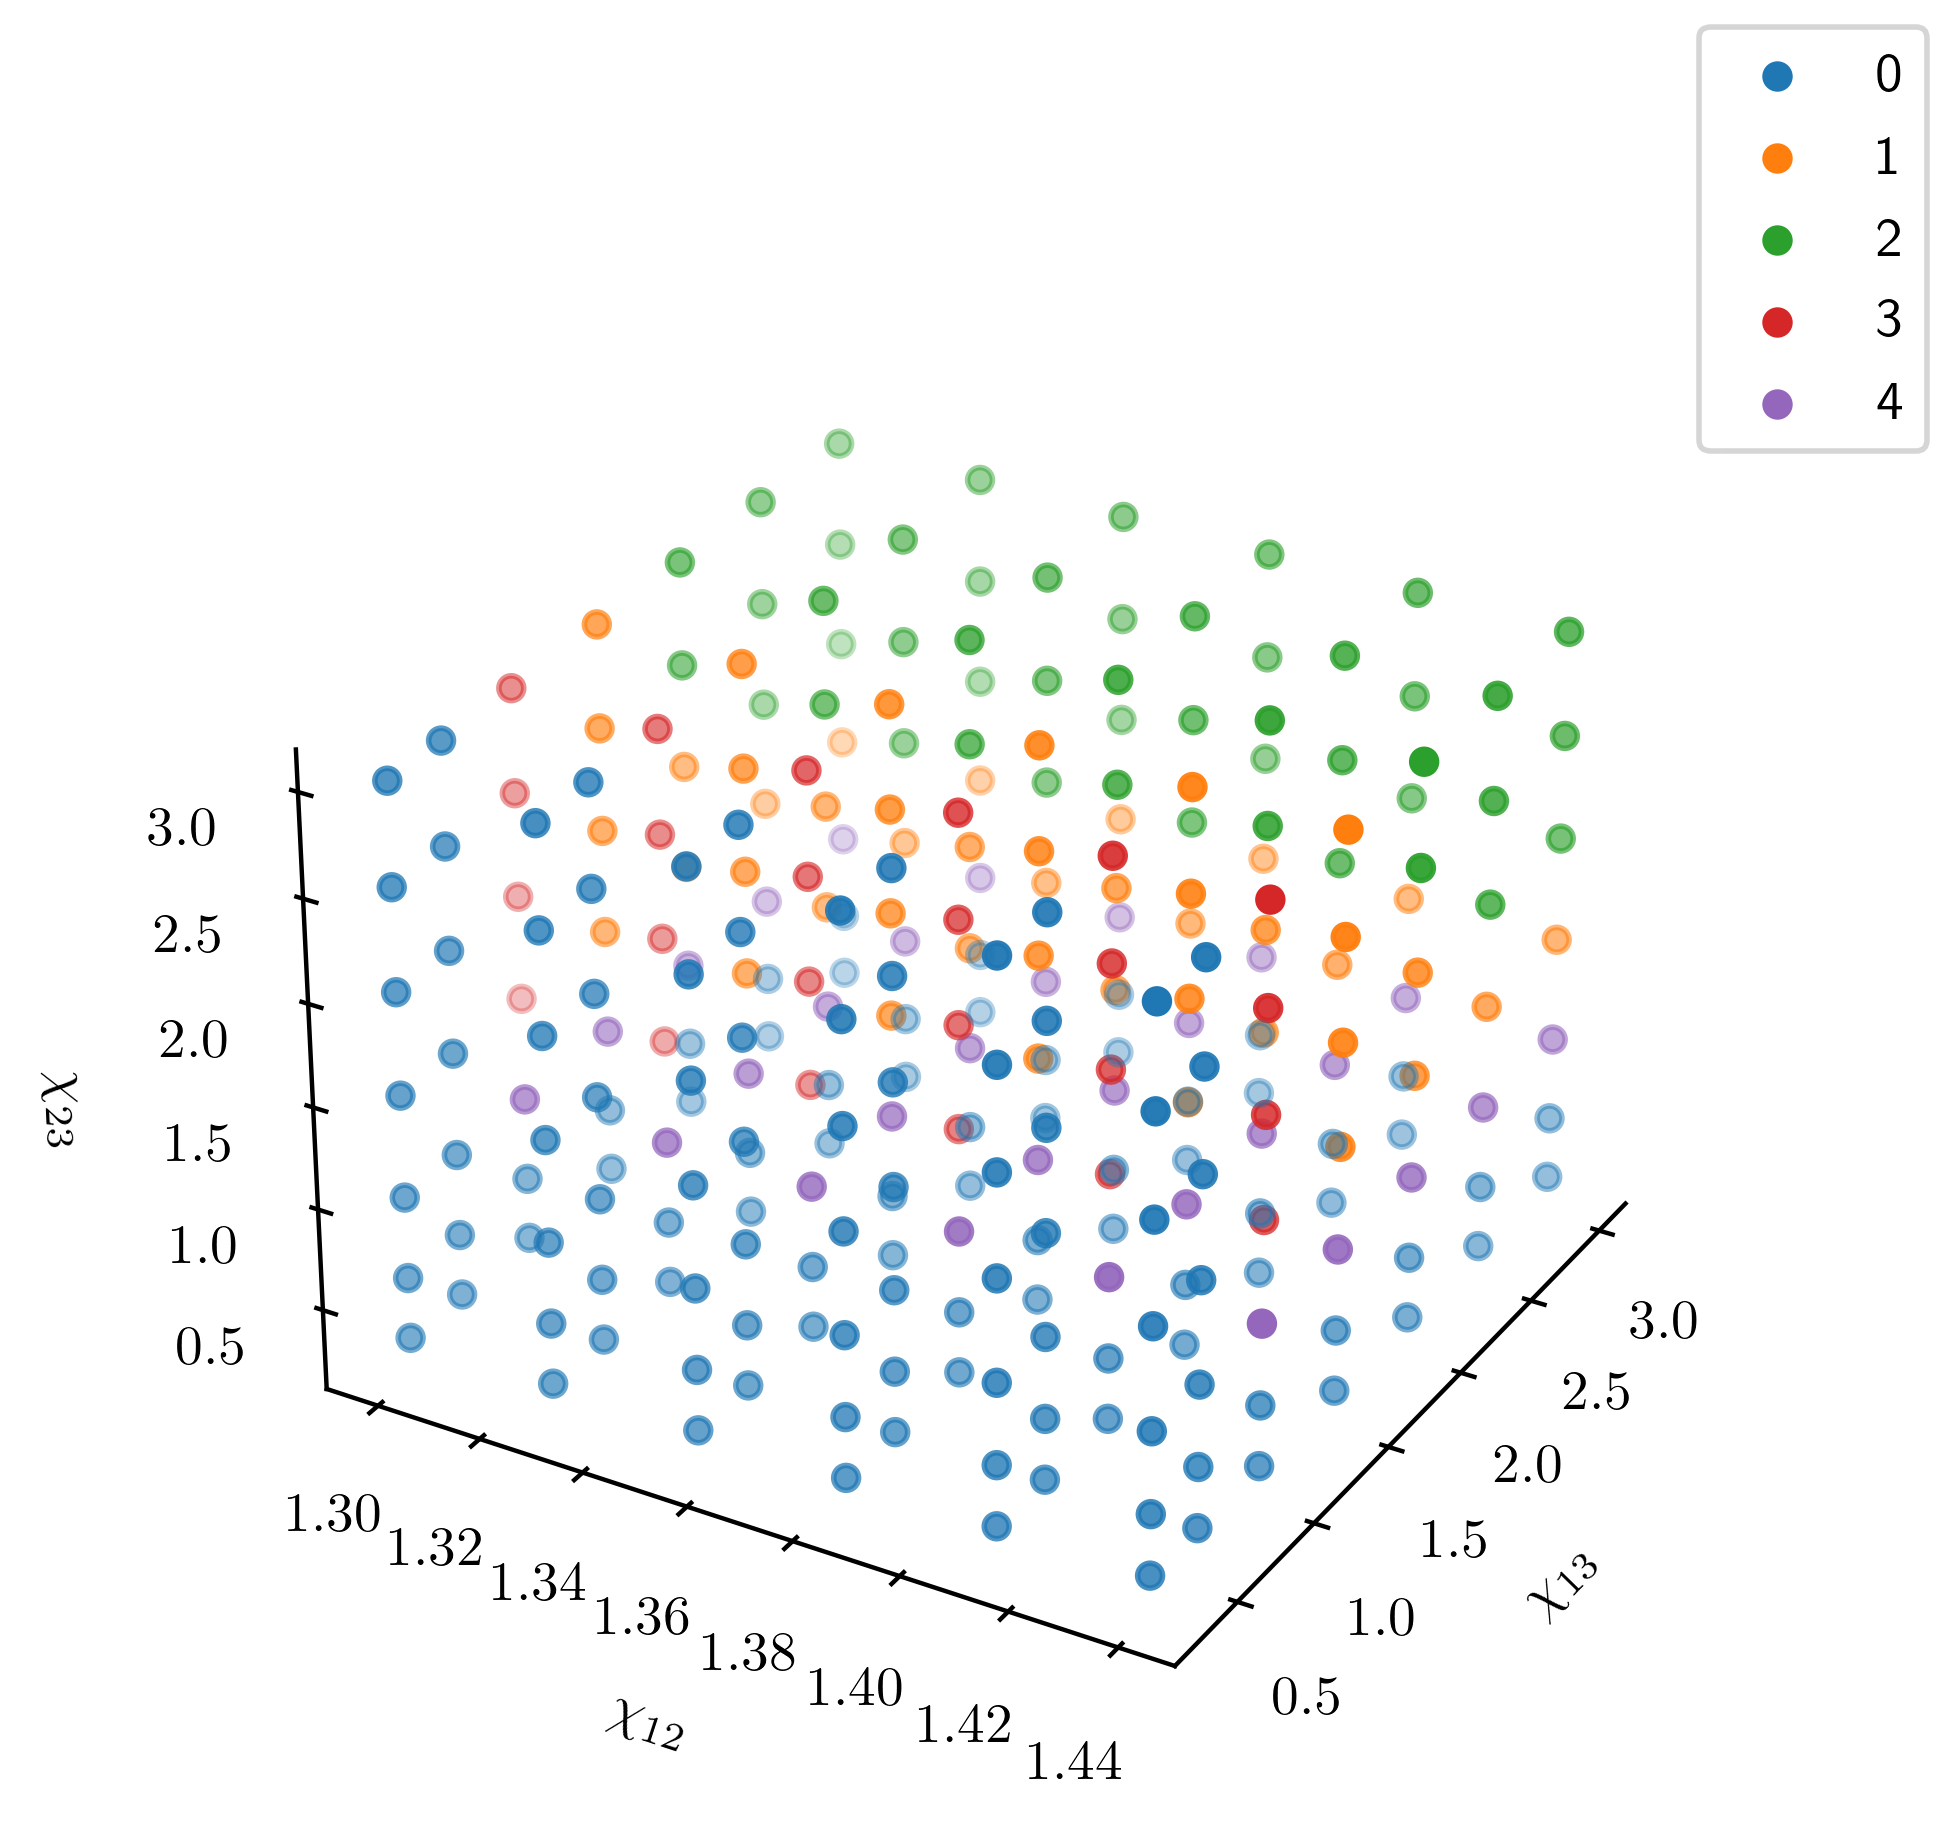
\includegraphics[width=\textwidth]{Chapter-4/figures/result2/result2_Synthetic_DesignSpace.png}
        \caption{}
        \label{fig:synth_designspace_3D}
    \end{subfigure}
    \hfill
    \begin{subfigure}[b]{0.4\textwidth}
        \centering
        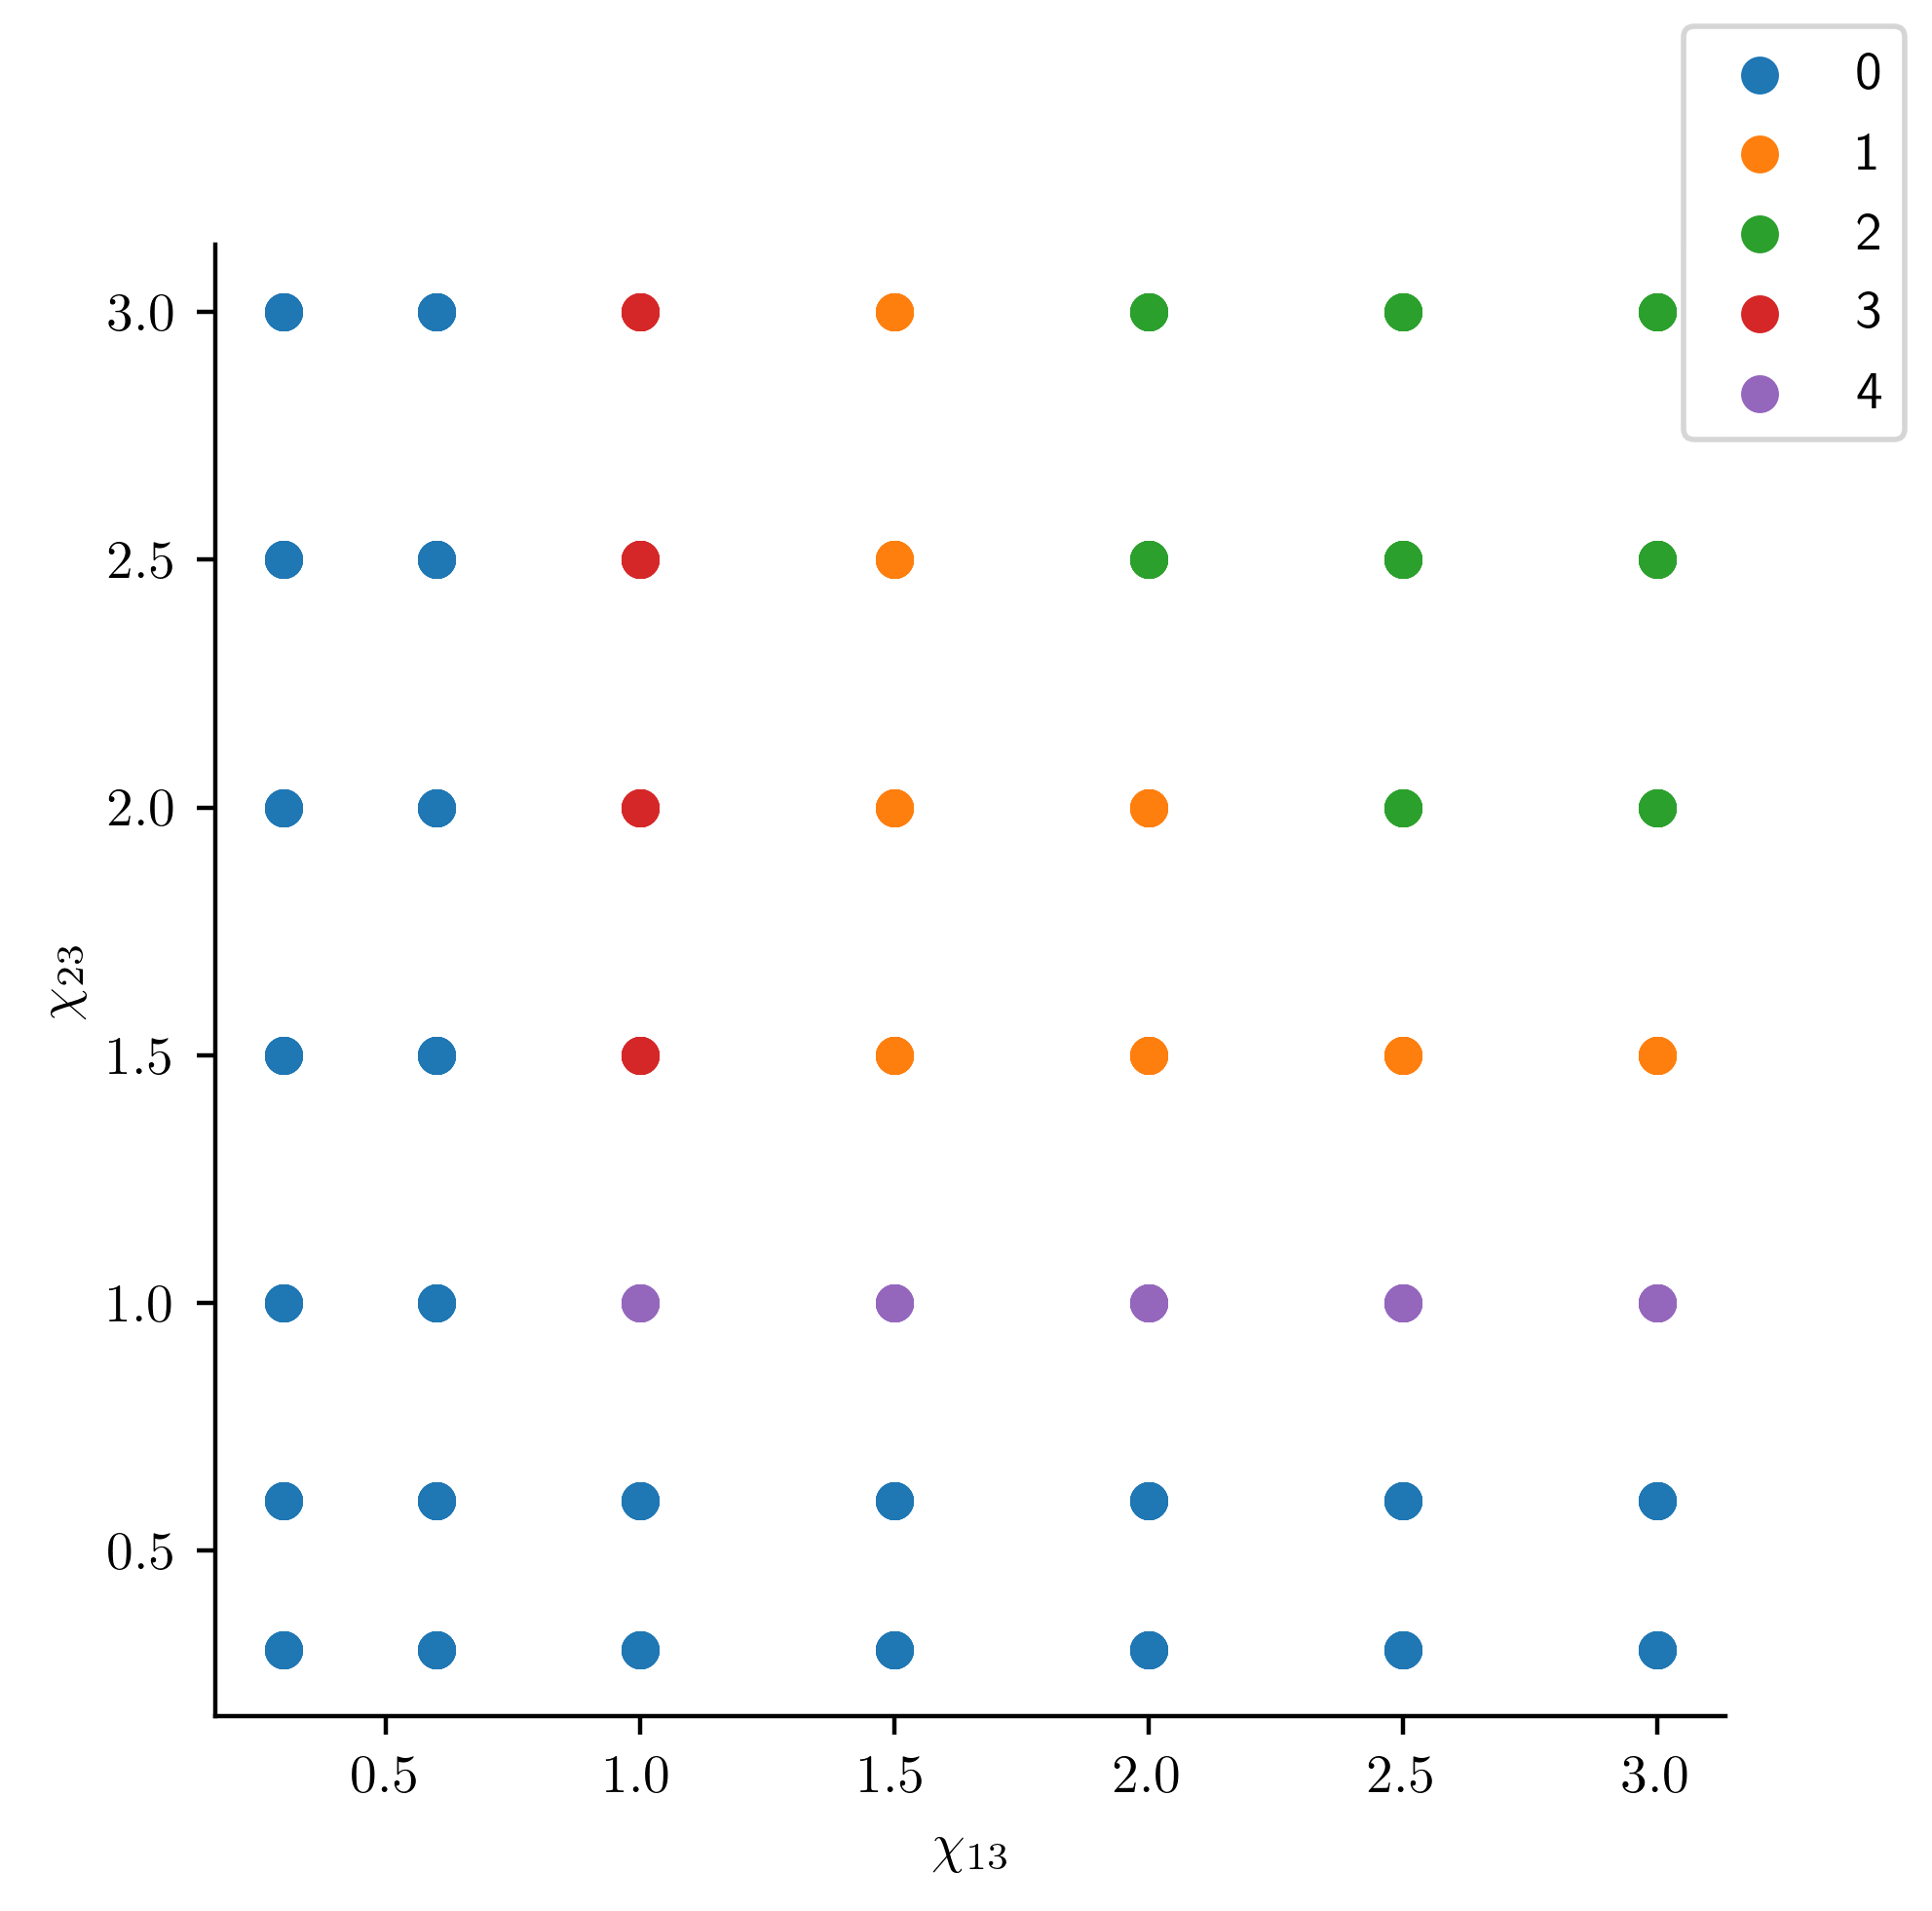
\includegraphics[width=\textwidth]{Chapter-4/figures/result2/result2_Synthetic_DesignSpace_2D.png}
        \caption{}
        \label{fig:synth_designspace_2D}
     \end{subfigure}
    \caption{Design space for model systems data set with points are color-coded with corresponding the cluster index of the phase diagram corresponds. (a) Input sampling space with \(\chi\) values as coordinates.Each point is colored based on their corresponding clustering label. (b) A radial trend in the clusters can be observed when visualizing the clusters on a two-dimensional projection of only \(\chi_{13}, \chi_{23}\).}
    \label{fig:synth_designspace}
\end{figure}

\section{Conclusions}
In this chapter, a high-throughput framework is introduced for phase diagram generation with the capabilities to evaluate for physical and computational accuracy. 
A data-analysis pipeline is used to perform initial screening of materials to identify subgroups there by decreasing the number of samples to be studied by an expert.
Applying the proposed methodology on two sets of material systems a framework is provided to derive potential design rules for solvent selection in OSC manufacturing.


\chapter{Conclusion}
The goal of the thesis has been to evaluate the use of data representations for application of machine learning to material discovery.
We introduced a distance measure learning approach into the data analytics for compositional libraries. 
A metric was learned from the data while leveraging the composition information about the design space. 
This is in contrast to the exhaustive search of distance measure that the state-of-the art.
We demonstrated the robustness of this approach for two case studies. 
First, we evaluated the framework using synthetically generated data sets of cyclic voltammetry measurements. 
Next, we applied the framework to labeled XRD data and constructed the phase diagram.
We showed that our method has the ability to identify regions in the design space where a systematic variation in design variable gives rise to systematic variation in response. 
Using a model electrochemistry data, we showed that a distance measure learned using our approach is at least as good as the metric chosen using an exhaustive search.
Through various test cases, we have shown that learning a similarity measure using MT-LMNN has the ability to automatically quantify the similarity measure for any given data set. This makes MT-LMNN a better alternative to an exhaustive search of complex and data specific metrics as well as a promising approach for automated distance learning for compositional libraries. 


In the second research task, we defined and evaluated a \(\mathcal{GP}\)-based oracle for materials discovery using cyclic voltammetry.
Next, we combined the oracle with a state-of-the-art active batch search to identify condition resulting in the targeted shape of CV curve. 
We demonstrated a robust high throughput combinatorial search to find the target responses using only \(<6\%\) of total number of CV experiments from the corresponding exhaustive search (with a discrete sampling of modest 5 levels per dimension). 
This work has implications in identification of characterization conditions where kinetic knowledge extraction from the cyclic voltammetry can be preformed more effectively. 
Specifically, we have illustrated a framework that can be used to identify S-shaped CV curves. 
Once S-shaped CV curve is obtained, a foot of the wave analysis can be applied ~\cite{FOWA} to extract rate constant for rate determining step, overpotential dependent turn over frequency etc.
In this sense our method has applications in accelerated knowledge extraction, with the application in screening for target catalysts including the bi-functional alkaline fuel cell catalysts that motivated this work.


A data exploratory analysis is introduced for phase diagram generation with the capabilities to evaluate for physical and computational accuracy. 
We use a data-analysis pipeline to perform initial screening of materials to identify subgroups there by decreasing the number of samples to be studied by an expert.
We apply our methodology on two sets of material systems and provide a framework to derive design rules for solvent selection in OSC manufacturing.

%%%%%%%%%%%%%%%%%%%%%%%%%%%%%%%%%%%%%%%%%%%%%%%%%%%%%%%%%%%%%%%
% Appendices
%
% Because of a quirk in LaTeX (see p. 48 of The LaTeX
% Companion, 2e), you cannot use \include along with
% \addtocontents if you want things to appear the proper
% sequence. Since the PSU Grad School requires
%%%%%%%%%%%%%%%%%%%%%%%%%%%%%%%%%%%%%%%%%%%%%%%%%%%%%%%%%%%%%%%
\appendix
\chapter{Gaussian Processes Machinery}\label{appendix}
\section{Basis functions of \(\mathcal{GP}\) function space representation}
Suppose we want to model a function \(f\) based on some known values at the observed points~(training data). We use a non-linear transformation of input values~\(x\) given by \(\phi(x)\) and corresponding weights \(W\) to represent the parametric form of \(f\) as:

\[ f(x) &= \phi(x)^{\top} W \]

Using the \(\mathcal{GP}\) formulation, we assume that \(W\) are drawn from a Gaussian Process with zero mean and \(\Sigma_p\) covariance i.e. W\sim\(\mathcal{GP}\big(0,\Sigma_p\big)\). This results in a Gaussian distribution on the functions \( f\sim\mathcal{GP}\big( \mu(x), k(x,x') \big) \) which can be obtained using the following: 
\begin{align*}
    \mathbb{E}\big[f(x)\big] &= \mathbb{E}\big[\phi(x)^{\top}W\big] \\
                     &= \phi(x)^{\top}\mathbb{E}\big[W\big] \\
                     &= \mu(x)=0 \\
    \mathbb{E}\big[f(x)f(x')^{\top}\big] 
                    &=\mathbb{E}\big[\phi(x)^{\top}W(\phi(x)^{\top}W)^{\top}\big] \\
                    &=\mathbb{E}\big[\phi(x)^{\top}WW^{\top}\phi(x)\big] \\
                    &= \phi(x)^{\top}\mathbb{E}\big[WW^{\top}\big]\phi(x) \\
                    &= \phi(x)^{\top}\Sigma_p\phi(x) \\
                    &= k(x,x')
\end{align*}
where \(\mathbb{E}\big[. \big]\) denotes expectation. Above formulation implies that by defining \(k(x,x')\), we identify the corresponding basis functions of the function space representation.

\subsection{Computing Model Evidence Using Laplacian Approximation}
Traditionally, a $\mathcal{GP}$ model is defined using the marginal likelihood denoted \(p(\textbf{y}|\textbf{X},\theta,\mathcal{M})\). However, $\theta$ used in the marginal likelihood is itself a model parameter which needs to be marginalized. In Bayesian model selection realm, it is common to use model evidence which is marginal likelihood of a $\mathcal{GP}$ model marginalized over $\theta$ i.e. \[\text{Model Evidence:} \quad p(\textbf{y}|\textbf{X},\mathcal{M})=\int p(\textbf{y}|\textbf{X},\theta,\mathcal{M})p(\theta|\mathcal{M}) \diff{\theta}.\] 
Marginal likelihood is a special case of Bayesian model evidence with \[p(\theta|\mathcal{M})=\delta(\hat{\theta}), \hat{\theta}=\argmax_{\theta} \log p(\theta|\mathcal{D},\mathcal{M}). \] \[p(\theta|\mathcal{D},\mathcal{M})=p(\textbf{y}|\textbf{X},\theta,\mathcal{M})p(\theta|\mathcal{M})\]
This is equivalent to saying that the model exits only at one parameter space i.e. \(\theta=\hat{\theta}\). Marginal likelihood estimation (MLE) or Maximum a-posteriori (MAP) estimates are used to select a $\hat{\theta}$~\cite{gardner2015bayesian}.
A common approach is to approximate model evidence using Laplacian approximation. We give the details of the approximation here for completeness.
Since $\hat{\theta}$ is a maxima of \(p(\theta|\mathcal{D},\mathcal{M})\), it is also maxima of its log PDF \[q(\theta)=\log(p(\theta|\mathcal{D},\mathcal{M}))\]
Making a Taylor series approximation over $\hat{\theta}$, we get \[q(\theta)\approx q(\hat{\theta})+(\theta-\hat{\theta})\dot q(\hat{\theta})+\frac{1}{2}(\theta-\hat{\theta})^{2}\ddot q(\hat{\theta})\]
Noting \(\dot q(\hat{\theta})=0\), we get \[q(\theta)\approx \text{Constant} +\frac{(\theta-\hat{\theta})^{2}}{2 (\ddot q(\hat{\theta}))^{-1}} \] 
This is equivalent to approximating \[ p(\theta|\mathcal{D},\mathcal{M})\sim \mathcal{N}(\hat{\theta},-\nabla^{2} \log p(\theta|\mathcal{D},\mathcal{M})\vert_{\hat{\theta}})\]
% A Laplacian approximation to the theta posterior around $\hat{\theta}$ as a mode results in the following: \[ p(\theta|\mathcal{D},\mathcal{M})\sim \mathcal{N}(\hat{\theta},-\nabla^{2} \log p(\theta|\mathcal{D},\mathcal{M})\vert_{\hat{\theta}}). \]
This will also result in an approximation to model evidence : 
\begin{align*}
   p(\textbf{y}|\textbf{X},\mathcal{M}) &= \int \exp \log  p(\theta|\mathcal{D},\mathcal{M})\diff{\theta} \\
   & \approx \int \exp \Bigg( q(\hat{\theta}) +\frac{(\theta-\hat{\theta})^{2}}{2 (\ddot q(\hat{\theta}))^{-1}}\Bigg)\diff{\theta}; \quad q(\theta)=p(\theta|\mathcal{D},\mathcal{M}) \\ 
   & = \exp(q(\hat{\theta}))\int \mathcal{N}\Big(\hat{\theta},A=-\ddot q(\hat{\theta})^{-1}\Big)\diff{\theta} \\
   & = p(\hat{\theta}|\mathcal{D},\mathcal{M})(2\pi)^{\frac{d}{2}}|A|^{-\frac{1}{2}} \\
   & = p(\mathcal{D} | \hat{\theta}, \mathcal{M})p(\hat{\theta} | \mathcal{M})(2\pi)^{\frac{d}{2}}|A|^{-\frac{1}{2}} \\
    & = p(\textbf{y} | \textbf{X}, \hat{\theta}, \mathcal{M})p(\hat{\theta} | \mathcal{M})(2\pi)^{\frac{d}{2}}|A|^{-\frac{1}{2}} \\
\end{align*}
{We typically compute the log-probability:}
\begin{align*}
  \log p(\textbf{y}|\textbf{X},\mathcal{M}) \approx \log p(\textbf{y}|\textbf{X},\mathcal{M},\hat{\theta}) + \log p(\hat{\theta}|\mathcal{M}) \\
  + \frac{d}{2}\log(2\pi) -\frac{1}{2}\log(|A|)  
\end{align*}
Recall that commonly used Bayesian information criteria (BIC) is a special case of Laplacian approximation to model evidence. BIC assumes that number of trained samples \(N\rightarrow \infty \) giving rise to:
\begin{align*}
    \text{\textbf{BIC:}}  \log p(\textbf{y}|\textbf{X},\mathcal{M}) \approx \log p(\textbf{y}|\textbf{X},\mathcal{M},\hat{\theta}) - \frac{d}{2}\log(N)
\end{align*}

\subsubsection{Computing Hessian's of $\mathcal{GP}$ models}
Computing model evidence using a Laplacian approximation requires one to compute Hessian's of $\mathcal{GP}$ models with respect to parameter index $\theta$. 
In this work, we use A MATLAB code to compute Hessian's at the model $\hat{\theta}$ given the Hessian's of $\mathcal{GP}$ models that has been previously published\footnote{\url{https://github.com/rmgarnett/gpml_extensions}}. Mean function models used in this study are zero thus have trivial Hessian's. Hessian's of  covariance models used in this study can be computed analytically which we report here. We note that Hessian for a squared exponential covariance has been already incorporated in the MATLAB code published by Garnett et al, thus we only report on Hessian for Neural Network covariance model used. For mathematical convenience, we denote the covariance in~\cref{eq:covNNone} using $K$ with the parameter index being \(\theta=[\theta_1=\lambda ; \theta_2=\sigma_f^{2} ]\) where \( \Lambda=\lambda I\). The Hessian of $K$ w.r.t $\theta$ would then be:
\[
\begin{bmatrix} 
\pdv[2]{K}{\theta_1} & \pdv{K}{\theta_1}{\theta_2} \\
\pdv{K}{\theta_2}{\theta_1} & \pdv[2]{K}{\theta_2} 
\end{bmatrix}
\]
\begin{align*}
    \pdv[2]{K}{\theta_1} & = -\lambda \sigma_{f}^{2}\Big(2\lambda XY + \lambda^2 Y\pdv{X}{\lambda} + \lambda^2 X\pdv{Y}{\lambda} \Big) \\
    \pdv{K}{\theta_1}{\theta_2} & = 2\lambda \sigma_{f}^{2}\frac{1}{\sqrt{1-a^2}}\pdv{a}{\lambda} \\
    \pdv[2]{K}{\theta_2} & =4K \\
    \newline
    \pdv{a}{\lambda}(x_p,x_q) & = -\lambda a\Big( \frac{1}{1+\lambda^{2}+x^{T}_{p} x_{p}} + \frac{1}{1+\lambda^{2}+x^{T}_q x_q}\Big) \\
    \pdv{X}{\lambda} & = -2\lambda\Big(\frac{1}{(1+\lambda^{2}+x^{T}_{p} x_{p})^2} + \frac{1}{(1+\lambda^{2}+x^{T}_q x_q)^2}\Big) \\
    X & = \frac{a}{\sqrt{1-a^2}} \\
    Y & = \frac{1}{1+\lambda^{2}+x^{T}_{p} x_{p}} + \frac{1}{1+\lambda^{2}+x^{T}_q x_q} \\
    a & = \frac{1+x^{T}_px_q}{\sqrt{1+\lambda^{2}+x^{T}_{p} x_{p}}\sqrt{1+\lambda^{2}+x^{T}_q x_q}} \\
\end{align*}

\subsection{Computing Model Posterior}
Once we have computed model evidence using the tools introduced in earlier sections, we can compute the model posterior $p(\mathcal{M}\vert \mathcal{D})$ which signifies the probability of a model $\mathcal{M}$ being the correct model given the data $\mathcal{D}$. Taking the logarithm of~\Cref{eq:postM} we get for model $\mathcal{M}_j,j\in \{1,2,...,m\}$. 
\newline

\begin{align*}
    \log p(\mathcal{M}_j\vert \mathcal{D}) & = \log \Big(p(\textbf{y}\vert\textbf{
    X},\mathcal{M}_j)p(\mathcal{M}_j) \Big) \\
    & -  \log \sum_{i=1}^{m}\Big(p(\textbf{y}\vert\textbf{
    X},\mathcal{M}_i)p(\mathcal{M}_i) \Big) \\
    \log \sum_{i=1}^{m}\Big(p(\textbf{y}\vert\textbf{
    X},\mathcal{M}_i)p(\mathcal{M}_i) \Big) & = \log \Big( p(\textbf{y}\vert\textbf{
    X},\mathcal{M}_j)p(\mathcal{M}_j) \Big) \\ & + \log \Big[ 1+ \sum_{i\neq j}^{m-1}\frac{p(\textbf{y}\vert\textbf{
    X},\mathcal{M}_i)p(\mathcal{M}_i)}{p(\textbf{y}\vert\textbf{
    X},\mathcal{M}_j)p(\mathcal{M}_j)} \Big] \\
    \log p(\mathcal{M}_j\vert \mathcal{D}) & = -\log \Big[ 1+ \sum_{i\neq j}^{m-1}\frac{p(\textbf{y}\vert\textbf{
    X},\mathcal{M}_i)p(\mathcal{M}_i)}{p(\textbf{y}\vert\textbf{
    X},\mathcal{M}_j)p(\mathcal{M}_j)} \Big] \\
    \quad p(\mathcal{M}) &= 1/m ~(\text{Assuming uniform distribution for the models}) \\
    \log p(\mathcal{M}_j\vert \mathcal{D}) & = -\log \Big[ 1+ \sum_{i\neq j}^{m-1}\frac{p(\textbf{y}\vert\textbf{
    X},\mathcal{M}_i)}{p(\textbf{y}\vert\textbf{
    X},\mathcal{M}_j)} \Big] \\
\end{align*}


\chapter{Dimensionality Reduction and Clustering}\label{appendixB}
\section{Dimensionality reduction}
Dimensionality reduction can be used to analyze the extensive data generated by projecting the data into lower dimensions while minimizing the loss of information (such as a similarity measure, correlation between data points). 
For example, consider each data point to be an image of a ternary phase diagram represented in pixel coordinates \(\mathbb{R}^{4096}\). 
Our goal is to identify a lower dimensional embedding, preferably in two or three.

Principal Component Analysis~(PCA) is the most commonly used dimensionality reduction method that projects a data matrix \(X\in \mathbb{R}^{n \times D}\) of \(n\) data points in  with each row corresponding to a D-dimensional sample into lower dimensions. 
The goal in PCA is to find a linear projection \(Y\) of the samples into a dimension \(d\) that is much lower than original dimension \(D\) while maximizing variance of data represented by \(X\) in \(Y\). 
PCA can be performed on \(X\) using an equivalent dual formulation in terms of singular value decomposition of \(X\) after mean centering~\cite{ESL}. 
In essence, PCA simply finds a nested-sequences of \textit{linear} sub-spaces passing through the mean of the data.
Given \(n\) \(p\)-dimensional points \(x_1,x_2,\dots,x_N \in X\), PCA computes a rank-q linear map \(f(\lambda, \mu) = \mu + V_q\lambda\) parameterized by \(\lambda, \mu\). 
The linear map \(f(\lambda, \mu)\) is optimized to minimize the reconstruction error defined by~\Cref{eq:pcaloss}.
\begin{align}\label{eq:pcaloss}
    \mathcal{L}_{pca}:=\min_{\mu, {\lambda_i}, V_q} \sum_{i=1}^{N} \norm{x_i - \mu -V_q\lambda_i}
\end{align}
where \(\norm{.}\) is Euclidean norm. 
\Cref{eq:pcaloss} can be optimized by solving for \(\pdv{\mathcal{L}_{pca}}{\mu}=\pdv{\mathcal{L}_{pca}}{\lambda}=0\) and obtain~\Cref{eq:pcaoptims} with \(\bar{x} =\frac{1}{N} \sum_{i=1}^{N} x_i \)
\begin{align}
    \mu &= \bar{x} \nonumber \\
    \lambda &= V_{q}^{T}(x_i - \bar{x}) \label{eq:pcaoptims}
\end{align}
Substituting the optimized values of \(\mu, \lambda\) in~\Cref{eq:pcaloss}, we get the loss function in terms of only \(V_q\)~\Cref{eq:pcaeigprob} that can be solved using:
\begin{align}
    \mathcal{L}_{pca}&:=\min_{V_q} \sum_{i=1}^{N}\norm{(x_i - \bar{x}) - V_{q}V_{q}^{T}(x_i - \bar{x})} \nonumber \\
    &=\min_{V_q} \sum_{i=1}^{N}\norm{\Tilde{x_i} - V_{q}V_{q}^{T}\Tilde{x_i}} \label{eq:pcaeigprob}
\end{align}

i.e. for any given mean centered \(p\) dimensional vector \(\Tilde{x_i}\); the solution of \Cref{eq:pcaeigprob} is a \(V_q\) that projects \(\Tilde{x_i}\) orthogonally to a sub-space spanned by columns of \(V_q\).
Thus the above formulation is same as a \textit{singular value decomposition} of the data matrix \(X\in \mathbb{R}^{N\times p}\) as \(X = UDV^T\) and the first \(q\) columns of \(V\) is compose required \(V_q\). 

Typically, the notion of explained variance defined using the Eigen values of the covariance matrix is used to determine number of dimensions \(d\) for the target lower dimensional Euclidean space \(Y\).
This because, \Cref{eq:pcaeigprob} is also the SVD of \(S = XX^{T} = \frac{1}{N}VD^2V^T\).
For any Eigen vector \(e\) of \(S\) and we get the following:
\begin{align}
    e^TSe &= e^T (\mathbb{E}(XX^T)-\mathbb{E}(X)\mathbb{E}(X^T))e \nonumber \\
    &= \mathbb{E}((e^TX)(e^TX)^T)-\mathbb{E}(e^TX)\mathbb{E}(e^TX)^T) \nonumber \\
    &= \text{Var}(e^TX)
\end{align}

Note that \(\text{Var}(e^TX)e = ee^TSe = Se\) since Eigen vectors are orthonormal i.e. \(ee^T=I\).
Thus, the Eigen values of \(S\) are variance of data points projected along their respective Eigen vectors. 


When a vector like representation of data is not available but a notion of (dis)similarity is available, a Multi-dimensional Scaling~(MDS) approach is used. 
We assume that the similarity values define a metric space and would like to find an embedding of the unknown metric space into Euclidean such that the distances are same.
MDS allows us to find a lower dimensional embedding that preserves the pair-wise similarities between points defined a square similarity matrix~(\(S\)) to euclidean distances in the lower dimensions. 
Similar to PCA, MDS can also be formulated as a matrix decomposition problem when \(s_{ij}\in S\) represents \(D\)-dimensional Euclidean distance between two points \(i,j\)~\cite{ESL}. 
Suppose \(y_1,y_2,y_3,\dots,y_n \in \mathbb{R}^d\) be a lower dimensional coordinate representation of a high dimensional data in \(X\in \mathbb{R}^D\) for which have pari-wise similarity matrix \(S \in \mathbb{R}^{n \times n}\). 
The goal in MDS is to find a map \(f: Y \rightarrow X\) from observed data to preserve the pairwise similarities. The optimization problem of MDS is defined using a stress function~\cref{eq:mdsloss} that can be solved using a gradient descent algorithm starting from a random set of points for \(Y\in\mathbb{R}^d\).
\begin{align}\label{eq:mdsloss}
    \mathcal{L}_{mds}:= \sum_{i\neq j}(s_{ij} - \norm{z_i - z_j})^2
\end{align}
when the similarity matrix~\(S\) is composed of Euclidean norm between high-dimensional points, PCA and (classical)MDS are equivalent~\cite{ESL}.

Often times it is useful to make an assumption that we only want to capture the \textit{local} similarity in \(S\) especially when the target embedding the space is Euclidean.
This means that we assume that the metric space underlying \(S\) has a manifold structure (locally similar to flat Euclidean space but globally curved).
Popular methods that use manifold assumption for dimensionality reduction include Isomap~\cite{Isomap} and LLE~\cite{LLE}. 
The goal of Isomap algorithm is to preserve approximate manifold geodesics (i.e. the shortest paths between any two points) in lower dimensions by first constructing a neighborhood graph (such that we only care about local similarities) of the input data~(typically a D-dimensional point cloud) and approximating geodesics~\(g_G\) with shortest path distances between two points. 
MDS is then used to obtain a low dimensional embedding that preserves \(g_G\). 
Isomap approximates global geometry of the embedded manifold by mapping both nearby and faraway points to the respective counterparts in the desired lower dimensional embedding~\cite{IsomapV2}. 
Computing coordinate representation is similar to MDS but the map \(f\) is restricted to being an isometric embedding that preserves infinitesimal lengths and angles in sense of Riemannian geometry. 
A consequence of isometric restriction on \(f\) is that it preserves geodesics i.e. shortest paths between any two points in \(X \in\mathbb{R}^D\). 
Global geometry~(i.e. metric information) of \(X\) is computed by replacing the pairwise distances with shortest paths using a neighborhood graph~(such as k-nearest neighbor graph for a user defined k).
Note that explained variance for metric embedding methods presented above would be calculated using a correlation coefficient between the metric in \(M\) and Euclidean distance metric of \(Y\)~\cite{Isomap}.

\section{Clustering}
Another approach to understand large amounts data involves usage of clustering methods to identify sub-groups with close similarities to the points with in a group but highly dissimilar across. 
In this section, we provide a brief overview of various clustering methods. 
For detailed discussion on clustering analysis and algorithms, readers are referred to~\cite{ESL}. 

Similar to MDS, notion of similarity plays a key role in cluster analysis of a data set and defines membership (corresponding to a group or subset) criteria. 
We are interested in clustering data based on a pre-computed similarity between phase diagrams. 
We therefore review clustering method that work on using only a matrix of similarities given in \(S\) namely \textit{k-medoids} and \textit{spectral clustering}. 
\textit{k-medoids} clustering is a generalization of k-means clustering when the only data available is a similarity matrix \(S\). 
In contrast to k-means algorithm where mean observation points are used as cluster centers, \textit{k-medoids} aims to find k observed points that minimize with-in cluster dissimilarities~\cite{ESL}. 
In this thesis we used a \textit{spectral clustering} method where the clusters are associated with subsets of a graph that minimize variation of a function within in the subset and maximize across ~\cite{SpectralClustering}. 
The approach involves computing a graph Laplacian defined as \(L = D-A\) where \(D\) is degree matrix and \(A\) is the adjacency matrix obtained from \(S\).
Suppose we have a signal sampled at the nodes of the graph for an underlying function \(f\), we have the following identity:
\begin{align}
    f^T L f &= \frac{1}{2}\sum w_{ij}(f_i -f_j)^2 \nonumber \\
            &= \frac{1}{2}\sum \left(\frac{f_i -f_j}{s_{ij}}\right)^2 \\
\end{align}
The above identify should also motivate the name "Laplacian" and the its interpretation as a measure of variation of function \(f\) along the graph.
Spectral clustering involves computing Eigen values of \(L\) thus equivalent to performing Fourier analysis on graphs with Eigen values corresponding to the frequencies~\cite{GFT}. 
Other methods include density based clustering such as DBSCAN and its variants.  

%%%%%%%%%%%%%%%%%%%%%%%%%%%%%%%%%%%%%%%%%%%%%%%%%%%%%%%%%%%%%%%
% ESM students need to include a Nontechnical Abstract as the %
% last appendix.                                              %
%%%%%%%%%%%%%%%%%%%%%%%%%%%%%%%%%%%%%%%%%%%%%%%%%%%%%%%%%%%%%%%
% This \include command should point to the file containing
% that abstract.
%\include{nontechnical-abstract}
%%%%%%%%%%%%%%%%%%%%%%%%%%%%%%%%%%%%%%%%%%%
} % End of the \allowdisplaybreak command %
%%%%%%%%%%%%%%%%%%%%%%%%%%%%%%%%%%%%%%%%%%%

%%%%%%%%%%%%%%%%
% BIBLIOGRAPHY %
%%%%%%%%%%%%%%%%
% You can use BibTeX or other bibliography facility for your
% bibliography. LaTeX's standard stuff is shown below. If you
% bibtex, then this section should look something like:
    \begin{singlespace}
       \bibliographystyle{unsrt}
       \phantomsection \addcontentsline{toc}{chapter}{Bibliography}
       \bibliography{ref}
    \end{singlespace}

%\begin{singlespace}
%\begin{thebibliography}{99}
%\addcontentsline{toc}{chapter}{Bibliography}
%\frenchspacing

%\bibitem{Wisdom87} J. Wisdom, ``Rotational Dynamics of Irregularly Shaped Natural Satellites,'' \emph{The Astronomical Journal}, Vol.~94, No.~5, 1987  pp. 1350--1360.

%\bibitem{G&H83} J. Guckenheimer and P. Holmes, \emph{Nonlinear Oscillations, Dynamical Systems, and Bifurcations of Vector Fields}, Springer-Verlag, New York, 1983.

%\end{thebibliography}
%\end{singlespace}

\backmatter

% Vita
% \vita{SupplementaryMaterial/Vita}

\end{document}

